%
% main.tex
%

%!TEX root = main.tex
%
% config.tex
%

\documentclass[11pt,a4paper,titlepage]{report}

\usepackage[pdfpagelabels]{hyperref}
\usepackage[utf8]{inputenc}

\usepackage
{
	makeidx,
	url,
	amsmath, 
	amssymb, 
	amsthm,
	mathrsfs,
	tikz,
	tikz-cd,
	chngcntr,
	apptools,
	cleveref,
	enumitem,
	cite,
	algorithm,
	algpseudocode,
	lmodern
}

% \usepackage[nottoc]{tocbibind}
\usepackage{etoolbox}
\makeatletter
\patchcmd{\l@chapter}{1.0em}{0.8em}{}{}
\makeatother

\usepackage{tikz-3dplot/tikz-3dplot}
\usepackage{pgfplots}
\usetikzlibrary{shapes}
\tdplotsetmaincoords{60}{0}
\usetikzlibrary{arrows}
\usetikzlibrary{shapes.geometric}

% \pgfplotsset{compat=1.13}
\pgfplotsset{compat=1.12}

\author{Raoul Wols}
\title{Master's Thesis}
\date{\today}

\theoremstyle{plain}
	\newtheorem{theorem}{Theorem}
	\counterwithin{theorem}{section} % important bit
	\newtheorem{lemma}[theorem]{Lemma}
	\newtheorem{proposition}[theorem]{Proposition}
	\newtheorem{corollary}[theorem]{Corollary}
	\newtheorem{claim}[theorem]{Claim}
	\newtheorem{conjecture}[theorem]{Conjecture}

	\newtheorem*{theorem*}{Theorem}
	\newtheorem*{lemma*}{Lemma}
	\newtheorem*{proposition*}{Proposition}
	\newtheorem*{corollary*}{Corollary}
	\newtheorem*{claim*}{Claim}
	\newtheorem*{conjecture*}{Conjecture}

\theoremstyle{definition}
	\newtheorem{definition}[theorem]{Definition}
	\newtheorem{example}[theorem]{Example}
	\newtheorem{exercise}{Exercise}
	\newtheorem{fact}[theorem]{Fact}
	\newtheorem{question}[theorem]{Question}
	\newtheorem{construction}[theorem]{Construction}

	\newtheorem*{definition*}{Definition}
	\newtheorem*{example*}{Example}
	\newtheorem*{exercise*}{Exercise}
	\newtheorem*{fact*}{Fact}
	\newtheorem*{question*}{Question}
	\newtheorem*{construction*}{Construction}

\theoremstyle{remark}
\newtheorem{remark}[theorem]{Remark}
\newtheorem{note}[theorem]{Note}

\AtAppendix{\counterwithin{theorem}{section}}
\AtAppendix{\counterwithin{exercise}{section}}

\newcommand{\N}{\mathbb{N}}
\newcommand{\Z}{\mathbb{Z}}
\newcommand{\Q}{\mathbb{Q}}
\newcommand{\R}{\mathbb{R}}
\newcommand{\C}{\mathbb{C}}
\newcommand{\NEEDREF}{\begin{color}{red}{\texttt{REF?}}\end{color}}
\newcommand{\TODO}{\begin{color}{red}{\texttt{TODO}}\end{color}}

\newcommand{\axiomnumbering}[1] {($#1 \arabic* $)}
\newcommand{\romansmallnumbering}{(\roman*)}


\DeclareMathOperator{\pr}{pr}
\DeclareMathOperator{\im}{im}
\DeclareMathOperator{\lcf}{lcf}
\DeclareMathOperator{\Int}{int}
\DeclareMathOperator{\ST}{\mu}
\DeclareMathOperator{\st}{star}
\DeclareMathOperator{\Sym}{Sym}
\DeclareMathOperator{\Stab}{Stab}
\DeclareMathOperator{\id}{id}
\DeclareMathOperator{\Hom}{Hom}
\DeclareMathOperator{\Iso}{Iso}
\DeclareMathOperator{\Aut}{Aut}
\DeclareMathOperator{\Sing}{Sing}
\DeclareMathOperator{\lcm}{lcm}
\DeclareMathOperator{\Spec}{Spec}
\DeclareMathOperator{\Sh}{Sh}
\DeclareMathOperator{\verteq}{\rotatebox{90}{=}}
\DeclareMathOperator{\op}{op}
\DeclareMathOperator{\Sub}{Sub}
\DeclareMathOperator*{\colim}{colim}
\DeclareMathOperator{\cod}{cod}
\DeclareMathOperator{\dom}{dom}
\DeclareMathOperator{\eval}{eval}
\DeclareMathOperator{\tr}{tr}
\DeclareMathOperator{\supp}{supp}

\newcommand{\HomLHOverXC}[2]{\Hom_{\mathbf{LH}/X_{\mathbf{C}}}\left(#1, #2\right)}
\newcommand{\uHomLHOverXC}[2]{\underline{\Hom}_{\mathbf{LH}/X_{\mathbf{C}}}\left(#1, #2\right)}


\includeonly
{
	introduction,
	ToposTheory,
	thefundamentalgroup,
	simplicialcomplexes,
	etalefunctor,
	isomorphism,
	outlook
}

\makeindex

\begin{document}

	\thispagestyle{empty}
	\vspace*{7em}
	\begin{center}
	{\large\bf R.A.C.H. Wols\par} \vspace{3em} {\LARGE\bf A McCord Functor for Alexandroff Categories\par} \vspace{3em} {\large\bf
	Master thesis\par} \vspace{1em} {\large\bf Thesis advisor:
	Dr. O.D. Biesel \par} \vspace{3em} {\large\bf July 7, 2016\\
	master exam: July 15, 2016\par}\vfill
	
\includegraphics{ulzegel.pdf}\\
	\vspace{2em}
	{\large\bf Mathematisch Instituut, Universiteit Leiden}
	\end{center}


	\clearpage

	\begin{abstract}
	We shall generalize the construction of McCord's weak homotopy equivalence between the realization of the nerve of a finite poset and the original poset to Alexandroff categories and the induced toposes between them. For this, we shall construct a functor, called the McCord functor, which will give us the basis for a geometric morphism. Finally, we attempt to find sufficient conditions for flatness. The resulting geometric morphism will provide an equivalence of categories on the level of locally constant finite objects.
	\end{abstract}

	\thispagestyle{empty}
	\null\vfill
	{
		\raggedright
		{
			\Huge
			\itshape
				What I cannot create, \\
				I do not understand.
			\par
			\bigskip
		}
		\bigskip
		\bigskip
		\raggedleft
		\Large
		\MakeUppercase
		{
			Richard Feynman
		}
		\par
	}

	\vfill
	\vfill

	\clearpage

	\newpage
	
	\addtocontents{toc}{\protect\enlargethispage{\baselineskip}}
	\tableofcontents
	\thispagestyle{empty}

	\newpage
	\clearpage
	\pagenumbering{roman} 

	%!TEX root = main.tex
%
% introduction.tex
%

\chapter{Introduction}

\section{Outline}

Chapter 1 of this thesis gives a light introduction to the subject ending with \cref{eq:intro-question}.
After that, the general flow of this thesis is divided into two parts. The first part, chapters 2 and 3, deal with topos theory. It sets up some basic definitions, theorems and propositions. There is basically no original work in these two chapters, except at the end of chapter 3, where we prove \cref{prop:locally constant iff every restriction map is a bijection}. This result will be used in chapter 6.

The second part of this thesis consists of the theory of simplicial sets. This is devoted to chapter 4. Half of this chapter is preliminary theory and should be well-known. Section 4.4 is all original work, where we set up a framework to work with open sets in a geometric realization. This it to be used in chapter 5.
Chapter 5 is devoted to the construction of the McCord functor. This is all original work, so the proofs become somewhat detailed here.
Chapter 6 proves the equivalence of categories on the level of locally constant finite objects. This, too, is all original work. So again the proofs are detailed.
Chapter 7 ends with an outlook on what problems might be solved still.
The reader knowledgeable in both topos theory and simplicial sets may thus skip to section 4.4 and read on.
In summary, up to section 4.4 is preliminary text (with the exclusion of \cref{prop:locally constant iff every restriction map is a bijection}), while section 4.4 and on is original work.

The bibliography and index pages may be found at the end of the paper. They do not appear in the contents because they would not fit.

\newpage
\section{Prerequisites and Notation}

As for the prerequisites, it is assumed that the reader has a firm grasp on category theory. I contemplated whether to include all the relevant category theoretic definitions, but I refrained from doing so because the preliminary text is already substantial. Here are some notions which should be familiar. Category. Small category. Balanced category. Functor. Left exact functor. Right exact functor. Exact functor. Isomorphism-reflecting functor. Adjoint pair of functors. Monoid. Monomorphism. Epimorphism. Exponentials. Cartesian closed categories. (Finite) (co)limits.
Moreover, I assume that the reader has seen (pre)sheaves, and is familiar with the classic construction of turning a continuous map $f : X \to Y$ of spaces into an adjoint pair of functors $f_* \dashv f^*$.

\bigskip

The set $\N$ is the set of natural numbers including zero. 
The set $\Z$ is the set of all integers. $\R$ denotes the real numbers. If something is in boldface, for instance, $\mathbf{C}$, then this is always a category. If something is in scriptface, for instance, $\mathscr{E}$, then this is always a topos. Sheaves and presheaves will be denoted by $F,G,P,Q$, etcetera (so \emph{not} by $\mathcal{F}$, $\mathcal{G}$). Natural transformations are always greek small letters, for instance $\alpha, \eta, \varepsilon$. Every diagram that is drawn in this thesis is commutative, or will be proven to be commutative. If $F$ and $G$ are functors, the symbol $F \dashv G$ means that $F$ is the left adjoint of $G$, or equivalently, $G$ is the right adjoint of $F$. $\mathbf{Set}$ is the category of sets. $\mathbf{set}$ is the category of finite sets. $\mathbf{Top}$ is the category of topological spaces.

\newpage
\section{Acknowledgements}
\bigskip \bigskip

I want to seize this opportunity to thank my advisor Owen Biesel. The past year has been great and I am thankful to have worked on mathematical problems with you. Thank you for for the fun weekly meetings.

\bigskip

\bigskip

My deepest gratitude goes to my family and especially my parents. Their love and support has kept me going these past years. Their unbounded patience is a virtue which I hope to inherit some day.

\bigskip

\bigskip

Finally, my friends. Thank you. From Dordrecht, Rotterdam, Den Haag, Leiden, Amsterdam, and Utrecht. You know who you are. Couldn't have done it without you. I thank you for the shared experiences. For the troubles we got into. For the late nights. For the early mornings. The coffee breaks. The tea breaks. Dinners. For the milestones we made. The card games. The live stage. Lunches. Festivals. The music. You have all been such a central part of my life for a long time. I want to believe that your combined effort has made a better person. Let me raise the glass for the things that still lie ahead of us. Here's to you!

\newpage

\section{Motivation and Problem Statement}
Let $X$ be a finite connected $T_0$-space. Then we have a lattice of open subsets $\mathcal{O}(X)$. We may form the category of sheaves on this lattice. Let us denote it by $\Sh(\mathcal{O}(X))$. From a different viewpoint, $X$ can be regarded as a partially ordered set. Every partially ordered set is a category. So we may also form the presheaf category $\mathbf{Set}^{X^{op}}$. That is, $\mathbf{Set}^{X^{op}}$ is the category whose objects are functors $X^{op} \to \mathbf{Set}$ and whose morphisms are natural transformations between them. Observe that every point $x$ of the space $X$ has a minimal open neighborhood. Let us denote it by $U_x \subset X$. This thesis began with the following observation.

\begin{theorem}
\label{thm:intro-theorem}
Let $X$ be a finite $T_0$-space. Then there is an equivalence of categories
\[ \begin{tikzcd}
\Sh(\mathcal{O}(X)) \arrow[shift left=0.25em]{r}{\varphi} & \mathbf{Set}^{X^{op}} \arrow[shift left=0.25em]{l}{\psi} \end{tikzcd} \]
where the functor $\varphi$ sends a sheaf $F$ to the presheaf defined by
\[ \varphi(F)(x) = F(U_x), \qquad x \in X, \]
while the quasi-inverse functor $\psi$ sends a presheaf $P$ to the sheaf defined on the basis of opens $\{U_x : x \in X\}$ by
\[\psi(P)(U_x) = P(x). \]
\end{theorem}
\begin{proof}
The functors are each other's quasi-inverse once we show that $\varphi$ and $\psi$ are well-defined. Note that $x \leq y \iff U_x \subseteq U_y$, so that $\varphi$ is well-defined, and for every presheaf $P$ on $X$ the presheaf $\psi(P)$ is a sheaf on the basis $\{U_x : x \in X\}$. So after taking a projective limit it corresponds to a sheaf on all of $\mathcal{O}(X)$.
\end{proof}
Meanwhile there is the notion of the nerve of a category, to be defined in \cref{def:nerve of a category}. In the case of the poset $X$, the nerve $N(X)$ is simply the simplicial set defined by the $n$-chains of elements $(x_0 \leq \ldots \leq x_n)$, with $x_i \in X$. So there are $n$ less-than-or-equal-to signs together with $n+1$ elements $x_i \in X$ in such an $n$-chain. One should view such an $n$-chain as being an actual $n$-simplex. To get the $i$'th face of an $n$-chain, simply forget the element $x_i$ in the chain to get an $(n-1)$-chain. Similarly, one can turn an $n$-chain into a so-called degenerate $(n+1)$-chain by repeating the $i$'th element $x_i$. Every simplicial set has a so-called geometric realization, whereby we turn a simplicial set into a topological space. Let us denote that space by $|NX|$. Concretely, elements of $|NX|$ are equivalence classes of pairs $[\sigma, t]$ where $\sigma = (x_1,\ldots, x_n)$ is an $n$-simplex of $NX$ and $t$ is a point on the standard geometric $n$-simplex $\Delta^n \subset \R^{n+1}$. Two representatives $(\sigma,t)$ and $(\tau,s)$ are equivalent if and only if ``one is a face of the other'', that is, if one can find a sequence of ``taking faces'' which realizes $\sigma$ as a face of $\tau$, and the point $t$ is geometrically reduced alongside the face maps to the point $s$. All this will be made precise in chapter 4. In any case, notice that every such $n$-chain is totally ordered with a minimal element. If $t \in \Delta^n$, let us define the \emph{support} \index{support (classic)}of $t$ to be the set of indices
\[ \supp(t) := \{i : t_i > 0\}. \]
Then, \cite[Theorem 1.4.6]{barmak11} tells us that there is a continuous map
\[ \mu : |NX| \to X, \qquad [(x_0 \leq \ldots \leq x_n),t] \mapsto x_{\min \supp(t)}, \]
called the \emph{McCord map}, \index{McCord map}which moreover induces a weak homotopy equivalence
\[ \widetilde{\mu} : \pi_n(|NX|) \xrightarrow{\sim} \pi_n(X), \qquad n \geq 0. \]
Combining this with \cref{thm:intro-theorem}, we see that we have an adjoint pair of functors
\begin{equation}
\label{eq:intro-equation}
\begin{tikzcd}
\Sh(\mathcal{O}|NX|) \arrow[shift left=0.25em]{rr}{\mu_* \circ \varphi} & \; & \mathbf{Set}^{X^{op}} \arrow[shift left=0.25em]{ll}{\mu^* \circ \psi} \end{tikzcd}
\end{equation}
where the right adjoint $\mu_* \circ \varphi$ sends a sheaf $F$ on $|NX|$ to the presheaf defined by
\[ \left(\mu^{-1} \circ \varphi\right)(F)(x) = F\left( \mu^{-1} U_x \right), \qquad x \in X. \]
It turns out that categories such as in \cref{eq:intro-equation} may be regarded as ``spaces'', and with that notion comes the notion of a ``fundamental group''. Such fundamental groups are not merely groups, but are in fact profinite groups carrying topological structure. By general category yoga, we may dedude then, using \cite[Theorem 1.15]{lenstra08}, that the functor above induces an isomorphism of profinite groups
\[ \widehat{\pi}_1\left(|NX|, |p| \right) \cong \pi_1\left( \mathbf{Set}^{X^{op}}, p \right). \]
Here, the notion of a ``point'' $p$ will be defined in \cref{def:point of a topos}.

The small category $X$ is part of a (big) category called the category of all small categories (with functors between them as morphisms), denoted by $\mathbf{Cat}$. Moreover, it turns out that such an adjoint pair is so common that a theory around it was developed by Grothendieck and co. Let us call such an adjoint pair for which the left adjoint is left exact a \emph{geometric morphism}. The precise definition is given in \cref{def:geometric morphism}.

\begin{question}
\label{eq:intro-question}
For which (connected) categories $\mathbf{C} \in \mathbf{Cat}$ does there exist a geometric morphism
\[
\begin{tikzcd}
\Sh(\mathcal{O}|N\mathbf{C}|) \arrow[shift left=0.25em]{rr} & \; & \mathbf{Set}^{\mathbf{C}^{op}} \arrow[shift left=0.25em]{ll} \end{tikzcd}
\]
which induces an isomorphism of profinite groups
\[ \widehat{\pi}_1(|N\mathbf{C}|, |p|) \cong \pi_1\left(\mathbf{Set}^{\mathbf{C}^{op}}, p \right)\; \]
and does all this even make sense?
\end{question}
The notion of connectedness is defined in \cref{def:connected topos}. What a fundamental group is is treated in chapter 3. Because geometric morphisms are so common, we'll denote them from now on with a \emph{single arrow} $\to$ instead of two arrows $\leftrightarrows$, but keep in mind that an adjoint pair is always meant.

This thesis will give a partial answer to \cref{eq:intro-question}. As it turns out, for \emph{every small category} there is at least a functor, dubbed the \emph{McCord functor} which looks like
\[ \ST : \mathbf{C} \to \mathbf{LH}/|N\mathbf{C}|. \]
Here, $\mathbf{LH}$ is the subcategory of $\mathbf{Top}$ consisting of all topological spaces together with \emph{local homeomorphisms} between them as morphisms (instead of just continuous maps). To make this $\ST$ work, we needed to introduce a certain class of categories called \emph{Alexandroff} categories which carry the right properties in order to turn $\ST$ into an equivalence of categories on the level of locally constant finite objects. The precise meaning of an Alexandroff category is given in \cref{def:alexandroff cat}. What locally constant finite objects are is explained in \cref{def:locally constant finite}.
We end here with the statement of the main result of the thesis, to be proved in \cref{coro:isomorphism of profinite groups}.
\begin{theorem}
Let $\mathbf{C}$ be a small connected Alexandroff category. Then there exists a geometric morphism
\[ \tau(\ST) : \Sh(\mathcal{O}|N\mathbf{C}|) \to \mathbf{Set}^{\mathbf{C}^{op}} \]
which induces an isomorphism of profinite groups
\[ \widehat{\pi}_1(|N\mathbf{C}|, |A|) \cong \pi_1\left(\mathbf{Set}^{\mathbf{C}^{op}}, A \right) \]
for every object $A \in \mathbf{C}$.
\end{theorem}



	\clearpage
	\pagenumbering{arabic} 

	%!TEX root = main.tex
%
% ToposTheory.tex
%

\chapter{Topos Theory Done Quick}
This preliminary section treats some basic concepts of topos theory. The main ingredients that we will need are the definition of a topos, the concept of a geometric morphism, the concept of points on a topos and the ``generalized $\otimes\text{-}\Hom$ adjunction''. We will follow mostly Chapter 2, 3, 4 and 7 of \cite{MacLaneMoerdijk91}. The book \cite{johnstone77} is also a good reference. This section is very terse and contains a lot of information. The reader is invited to consult the references.

\section{Basic Definitions}

We made an attempt to give the definition of a topos in its most elementary form, but it turned out that for the purposes of this thesis, it was not necessary to know the definition in its utmost generality. Because of this, we shall give two definitions; they are both instances of a more general concept of a topos. The interested reader is invited to read \cite{johnstone77} or \cite{MacLaneMoerdijk91}.

\begin{definition}
\index{presheaf topos}
\label{def:presheaf topos}
Let $\mathbf{C} \in \mathbf{Cat}$ be a small category. Recall that $\mathbf{C}^{op}$ denotes the opposite category. We call the category of set-valued functors
\[ [\mathbf{C}^{op}, \mathbf{Set}] = \mathbf{Set}^{\mathbf{C}^{op}} \]
a \emph{presheaf topos}.
\end{definition}

\begin{definition}
\index{Yoneda functor}
\label{def:Yoneda functor}
Let $\mathbf{C}$ be a category. The contravariant \emph{Yoneda functor} is defined as the functor which sends objects to representables. That is,
\[ \mathbf{y} : \mathbf{C} \to \mathbf{Set}^{\mathbf{C}^{op}}, \qquad A \mapsto \Hom_{\mathbf{C}}(-,A). \]
\end{definition}

Recall that if $X \in \mathbf{Top}$ and if $F : \mathcal{O}(X)^{op} \to \mathbf{Set}$ is a presheaf, then $F$ is called a \emph{sheaf} if every matching family has a unique amalgamation.

\begin{definition}
\index{sheaf topos}
\label{def:sheaf topos}
Let $X \in \mathbf{Top}$ be a topological space. The category of all sheaves
\[ \Sh(\mathcal{O}(X)) \]
is called a \emph{Grothendieck topos}.
\end{definition}
\begin{definition}
\label{def:Gset topos}
Let $G$ be a topological group. The category $G\text{-}\mathbf{Set}$ is the category of all sets with a continuous right $G$-action, together with equivariant maps respecting the continuous $G$ action between them. We call this a \emph{topos of $G$-sets}.
\end{definition}
In the special case that $G$ is discrete, it is in fact a presheaf topos: consider $G$ as a one-object category, call the object $\bullet$. For each $g \in G$, consider it as a morphism $g : \bullet \to \bullet$. Then $G$ is a groupoid. Take the presheaves on this groupoid. This is the same thing as $G\text{-}\mathbf{Set}$.
\begin{definition}
\index{topos}
\label{def:topos}
By a \emph{topos} we mean either a presheaf topos, a Grothendieck topos or a topos of $G$-sets, for some topological group $G$. A topos will always be denoted by $\mathscr{E}$ or $\mathscr{F}$.
\end{definition}

\begin{fact}[A topos is like the category of sets] Let $\mathscr{E}$ be a topos. Then $\mathscr{E}$ has all finite limits and all finite colimits, so in particular an initial object $0$ and a terminal object $1$. Every monic arrow is an equalizer. Every arrow both monic and epi is an isomorphism. $\mathscr{E}$ has exponentials. Every arrow $f$ factors as $f = m \circ e$, with $e$ epi and $m$ mono. For any object $B \in \mathscr{E}$, the slice category $\mathscr{E}/B$ is also a topos. Any arrow $k : A \to 0$ is an isomorphism. Any arrow $0 \to B$ is monic.
Any object $C \in \mathscr{E}$ has a monomorphism to an injective object. All of these facts can be found as theorems, lemma's and propositions in \cite[Chapter 3]{MacLaneMoerdijk91}.
\end{fact}

We shall see during the thesis that $\mathscr{E}$ is also like a ``space'', with ``points''.

% \begin{definition}[Elementary Topos]
% \label{def:elementary topos}
% An \emph{elementary topos} \index{elementary topos} is a category $\mathscr{E}$ with the following properties.
% \begin{enumerate}
% 	\item Every diagram $X \to B \leftarrow Y$ can be completed to a pullback diagram.
% 	\item $\mathscr{E}$ has a terminal object $1$.
% 	\item $\mathscr{E}$ has an object $\Omega$ and a monomorphism $\text{true} : 1 \rightarrowtail \Omega$ such that for any mono $m : S \rightarrowtail B$ there exists a \emph{unique} morphism $\chi_S : B \to \Omega$, called the \emph{characteristic} map \index{characteristic map} or \emph{classifying} \index{classifying map} map, such that
% 	\[ \begin{tikzcd}
% 	S \arrow{r} \arrow[swap,tail]{d}{m} & 1 \arrow[tail]{d}{\text{true}} \\
% 	B \arrow[swap]{r}{\chi_S} & \Omega
% 	\end{tikzcd} \]
% 	is a pullback diagram.
% 	\item For every $B \in \mathscr{E}$ we require an object $PB \in \mathscr{E}$, called the \emph{power object},\index{power object} and we require an arrow $\in_B : B \times PB \to \Omega$ such that for any morphism $f : B \times A \to \Omega$ there is a \emph{unique} arrow for which the following diagram commutes.
% 	\[ \begin{tikzcd}
% 	A \arrow[dashed, swap]{d}{\exists ! g} & B \times A \arrow{r}{f} \arrow[swap, dashed]{d}{1 \times g} & \Omega \arrow[equals]{d} \\
% 	PB & B \times PB \arrow[swap]{r}{\in_B} & \Omega
% 	\end{tikzcd} \]
% \end{enumerate}
% \end{definition}

% \begin{example}
% The category of sets $\mathbf{Set}$ is a topos. The slice category $\mathbf{Set}/X$ is a topos for every set $X$. If $\mathbf{C}$ is a small category, then the presheaf category $\mathbf{Set}^{\mathbf{C}^{op}}$ is a topos.
% \end{example}

\begin{definition}
\index{subobject}
\label{def:subobject}
A \emph{subobject} \index{subobject} of $B \in \mathscr{E}$ is an isomorphism class of monomorphisms $m : S \rightarrowtail B$. Two subobjects lie in the same isomorphism class if and only if there is an isomorphism between them making the obvious triangle commute. The set of subobjects is denoted by $\Sub_{\mathscr{E}}(B)$.
\end{definition}

\begin{definition}
\index{sieve}
\label{def:sieve}
Let $\mathbf{C}$ be a category and take an object $C \in \mathbf{C}$. By a \emph{sieve} we mean a subfunctor $S \subseteq \mathbf{y}(C)$.
\end{definition}

Among all objects in a topos is one which requires special attention. We shall construct it here using our definition of a topos, but we stress that in the elementary definition of a topos, it is \emph{part of the definition}.

\begin{construction}[$\Omega$ for presheaf toposes]
Suppose that $\mathscr{E}$ is a presheaf topos. Define a presheaf $\Omega$ as follows. For every object $C \in \mathbf{C}$, we set
\[ \Omega(C) = \{\text{sieves on $C$}\}. \]
If $f : D \to C$ is a morphism in $\mathbf{C}$, the restriction map $\Omega(f)$ is given by pulling back the sieve. Define a natural transformation $\text{true}:1 \to \Omega$ which on the component $C$ works by sending the unique element of $1$ to the maximal sieve $\mathbf{y}(C)$.
\end{construction}

\begin{construction}[$\Omega$ for sheaf toposes]
Suppose that $\mathscr{E}$ is a sheaf topos on a topological space $X$. Define a presheaf $\Omega$ on $\mathcal{O}(X)$ by
\[ \Omega(U) = \{W \mid W \subset U, \; W \text{ open in } X\}, \qquad U \in \mathcal{O}(X). \]
If $V \subset U$ are opens of $X$, the restriction map is given by intersecting with $V$. The so-constructed presheaf $\Omega$ is a sheaf by \cite[Theorem II.9.2]{MacLaneMoerdijk91}. Define a natural transformation $\text{true} : 1 \to \Omega$ which on the component $U \in \mathcal{O}(X)$ works by sending the unique element of $1$ to the element $U \in \Omega(U)$.
\end{construction}

\begin{construction}[$\Omega$ for $G$-sets]
Suppose that $\mathscr{E}$ is equivalent to $G\text{-}\mathbf{Set}$ for some topological group $G$. Take $\Omega = 1 \sqcup 1$ with trivial $G$-action and choose a monomorphism $\text{true} : 1 \to \Omega$.

\end{construction}

\begin{proposition}
For each object $A \in \mathscr{E}$ there is a natural isomorphism
\[ \Sub_\mathscr{E}(A) \cong \Hom_{\mathscr{E}}\left(A, \Omega \right) \]
\end{proposition}
\begin{proof}
Given a monomorphism $m : S \rightarrowtail A$, construct a classifying map. For the other way, take the pullback with the map $\text{true} : 1 \to \Omega$.
\end{proof}

Thus, $\Omega$ may be regarded as the representable object for subobjects. For this reason, we call it the \index{subobject classifier}\emph{subobject classifier}.

Before we move on to the next section, there is one construction which we'll use too.

\begin{definition}
\index{category of elements}
\label{def:category of elements}
Let $P \in \mathbf{Set}^{\mathbf{C}^{op}}$ be a presheaf. The \emph{category of elements}, denoted
\[ \int_\mathbf{C} P \]
is the category whose objects are pairs $(C,c)$ with $C \in \mathbf{C}$ and $c \in P(C)$. An arrow $f : (C,c) \to (C',c')$ is an arrow $f : C \to C'$ in $\mathbf{C}$ such that $c = P(f)(c')$, or in a more compact notation, such that $c = c' \cdot f$.
\end{definition}

There is an evident projection functor

\[ \pi_P : \int_{\mathbf{C}} P \to \mathbf{C}, \qquad (C,c) \mapsto C. \]
Thus, when composed with the Yoneda functor we have a functor back to the original presheaf topos that we started with, that is:
\[ \mathbf{y} \circ \pi_P : \int_{\mathbf{C}} P \to \mathbf{Set}^{\mathbf{C}^{op}}, \qquad (C,c) \mapsto \Hom_{\mathbf{C}}\left(-,C \right). \]

\begin{proposition}
\label{prop:every presheaf is a colimit of representables}
We have a natural isomorphism
\[ P \cong \colim \left( \mathbf{y} \circ \pi_P \right). \]
In other words, every presheaf is a colimit of representables.
\end{proposition}
\begin{proof}
This is \cite[Corollary I.3]{MacLaneMoerdijk91}.
\end{proof}

% If $B$ is an arbitrary object we have two projection maps $B \times B \to B$. The \emph{diagonal map} \index{diagonal map} is the map $\Delta_B : B \to B \times B$ with the property that composition with the two projections to $B$ give the identity $\id_B$. This shows that $\Delta_B$ is monic, so from the third axiom in \cref{def:elementary topos} we have a pullback diagram
% \[ \begin{tikzcd}
% B \arrow{r} \arrow[swap]{d}{\Delta_B} & 1 \arrow[tail]{d}{\text{true}} \\
% B \times B \arrow[swap, dashed]{r}{\delta_B} & \Omega
% \end{tikzcd} \]
% and thus from the fourth axiom we get a unique map
% \[ \begin{tikzcd}
% B \arrow[dashed]{r}{\{.\}_B} & PB
% \end{tikzcd}. \]
% We call the so-constructed map $\{\cdot\}_B$ the \emph{singleton map} \index{singleton map}, because for $\mathbf{Set}$ it is just the map which sends an element to the singleton set. We collect now some useful properties of elementary toposes.

% \begin{proposition}
% Let $\mathscr{E}$ be a topos. Then the following is true.
% \begin{enumerate}
% 	% \item For all objects $B \in \mathscr{E}$, $\{\cdot\}_B$ is monic.
% 	\item Every monic arrow is an equalizer.
% 	\item Every arrow both monic and epi is an isomorphism.
% 	\item $\mathscr{E}$ has exponentials.
% 	\item $\mathscr{E}$ has all finite colimits.
% 	\item Every arrow $f$ factors as $f = m \circ e$, with $e$ epi and $m$ mono.
% 	\item For any object $B \in \mathscr{E}$, the slice category $\mathscr{E}/B$ is also a topos.
% 	\item Any arrow $k : A \to 0$ is an isomorphism.
% 	\item Any arrow $0 \to B$ is monic.
% 	\item Any object $C \in \mathscr{E}$ has a monomorphism to an injective object.
% \end{enumerate}
% \end{proposition}
% \begin{proof}
% (1) is \cite[Lemma IV.1.1]{MacLaneMoerdijk91}. (2) and (3) are \cite[Proposition IV.1.2]{MacLaneMoerdijk91}. (4) is \cite[Theorem IV.2.1]{MacLaneMoerdijk91}. (5) is \cite[Corollary IV.5.4]{MacLaneMoerdijk91}. (6) is \cite[Proposition IV.6.1]{MacLaneMoerdijk91}. (7) is \cite[Theorem IV.7.1]{MacLaneMoerdijk91}. (8) is \cite[Proposition IV.7.4]{MacLaneMoerdijk91}. (9) is \cite[Corollary IV.7.5]{MacLaneMoerdijk91}.
% \end{proof}

% \section{Sheaves on a Site}

% This section introduces Grothendieck toposes.

% \begin{definition}
% Let $\mathbf{C}$ be a category and $C \in \mathbf{C}$.
% A \emph{sieve on $C$} \index{sieve} is a set $S$ of arrows with codomain $C$ such that
% \[ f \in S \text{ and the composite } f \circ h \text{ is defined implies } f \circ h \in S. \]
% \end{definition}
% Equivalently, a sieve $S$ on $C$ is a subfunctor of the Yoneda functor $\mathbf{y}(C)$.

% \begin{definition}
% \label{def:grothendieck topology}
% Let $\mathbf{C}$ be a category. A \emph{(Grothendieck) topology} \index{Grothendieck topology} is a function $J$ which assigns to every object $C \in \mathbf{C}$ a collection $J(C)$ of sieves on $C$ with the property that
% \begin{enumerate}
% 	\item[(non-emptyness)] the maximal sieve $t_C$ is in $J(C)$,
% 	\item[(stability)] if $S \in J(C)$, then for every $h : D \to C$ we have $h^*(S) \in J(D)$, and
% 	\item[(transitivity)] if $S \in J(C)$ and $R$ is a sieve on $C$ with the property that for all $h : D \to C$ in $S$ we have $h^*(R) \in J(D)$, then $R \in J(C)$.
% \end{enumerate} 
% \end{definition}

% A sieve $S$ is called a \emph{covering sieve} \index{covering sieve} if $S \in J(C)$ for some $C \in \mathbf{C}$.
% It's beneficial to define a basis for a Grothendieck topology in order to give one for practical purposes. It's only possible to define such a basis when $\mathbf{C}$ has pullbacks. In most applications the underlying category $\mathbf{C}$ does have pullbacks.

% \begin{definition}
% Let $\mathbf{C}$ be a category with pullbacks. A \emph{basis} \index{basis} for a Grothendieck topology is a function $K$ which gives for each object $C \in \mathbf{C}$ a collection $K(C)$ which consists of families of morphisms with codomain $\mathbf{C}$ with the property that
% \begin{enumerate}
% 	\item[(non-emptyness)] if $f : C' \to C$ is an isomorphism, then $\{f\} \in K(C)$,
% 	\item[(stability)] if $\{f_i : C_i \to D\}_{i \in I} \in K(C)$, then for every morphism $g : D \to C$ the collection of pullbacks $\{C_i \times_C D \to \}_{i \in I}$ is in $K(D)$, and
% 	\item[(transitivity)] if $\{f_i : C_i \to C\}_{i \in I}$ is in $K(C)$ and if for every $i \in I$ we have a family $\{g_{ij} : D_{ij} \to C_i\}_{j \in I_i}$, then the family of compositions $\{f_i \circ g_{ij} : D_{ij} \to C\}_{i \in I, j \in I_i}$ is in $K(C)$.
% \end{enumerate}
% \end{definition}
% A topology $J$ is not a basis. But if $K$ is a basis on $\mathbf{C}$, then $K$ generates a topology $J$ by saying that
% \[ S \in J(C) \iff \exists R \in K(C) : R \subseteq S. \]
 
% \begin{definition}
% \label{def:site}
% A \emph{site} \index{site} is a pair $(\mathbf{C},J)$ where $\mathbf{C}$ is a small category and $J$ is a Grothendieck topology. By abuse of notation, by $(\mathbf{C},K)$ we will also mean a site, where $K$ is a basis.
% \end{definition}

% \begin{example}
% The \emph{trivial topology} on $\mathbf{C}$ is the one in which the only covering sieves are the maximal sieves.
% \end{example}
% \begin{example}
% If $\mathbf{T}$ is a suitable subcategory of $\mathbf{Top}$ (for instance, separated Hausdorff spaces), then define a basis $K$ by $\{f_i : Y_i \to X\}_{i \in I} \in K(X) \iff$ every $Y_i$ is an open subset of $X$ with $f_i$ the natural inclusion.
% \end{example}
% \begin{example}
% Let $\mathbf{P}$ be a partially ordered set. If $p \in \mathbf{P}$ then a subset $D \subseteq \{q \in \mathbf{P} : q \leq p\}$ is said to be \emph{dense below $p$} if for any $r \leq p$ there is a $q \leq r$ with $q \in D$. Define the \emph{dense topology} on $\mathbf{P}$ by declaring
% \[ J(p) = \{D \mid q \leq p \text{ for all } q \in D \text{ and } D \text{ is a sieve dense below } p\}. \]
% \end{example}
% \begin{example}
% The \emph{atomic topology} on $\mathbf{C}$ is the one defined by
% \[ S \in J(C) \iff \text{ the sieve } S \text{ is not empty}. \]
% Here we require that every diagram $E \to C \leftarrow D$ in $\mathbf{C}$ can be completed to a commutative square (much weaker than the requirement of pullbacks).
% \end{example}
% \begin{example}
% Let $X$ be a scheme. Let $X_{\text{Zar}}$ be the category whose objects are all open sets $U \subset X$ and whose morphisms are the inclusion maps. Define the basis $K$ on $X_{\text{Zar}}$ by declaring
% \[ \{U_i \to U\}_{i \in I} \in K(U) \iff \bigcup_{i \in I} U_i = U. \]
% \end{example}
% \begin{example}
% Similarly, let $X$ be a scheme again. This time, let $X_{\text{et}}$ be the category whose objects are all etale morphisms of schemes $f : Y \to X$. Define the basis $K$ on $X_{\text{et}}$ by declaring
% \[ \{f_i : Y_i \to X\}_{i \in I} \in K(Y) \iff \bigcup_{i \in I}f_i(Y_i) = Y. \]
% \end{example}

% The point of defining a site is to define sheaves on that site. Let $(\mathbf{C},J)$ be a site. A presheaf $P$ on $\mathbf{C}$ is simply a functor $P : \mathbf{C}^{op} \to \mathbf{Set}$. 
% Now if $C \in \mathbf{C}$ is an object and $S \in J(C)$ is a covering sieve, let us define a \emph{matching family} \index{matching family} for $S$ to be a function which assigns to every element $f \in S$, where $f : D \to S$, an element $x_f \in P(D)$ such that
% \[ P(g)(x_f) = x_{f \circ g} \qquad \text{for all } g : E \to D \text{ in } \mathbf{C}. \]
% An \emph{amalgamation} \index{amalgamation} of a matching family is a single $x \in P(C)$ such that
% \[ P(f)(x) = x_f \qquad \text{for all } f \in S. \]
% \begin{definition}
% \label{def:presheaf is a sheaf iff every matching family has a unique amalgamation}
% The presheaf $P$ is called a $J$-\emph{sheaf}, \index{sheaf} or simply a \emph{sheaf}, if every matching family has a unique amalgamation. The full subcategory of $\mathbf{Set}^{\mathbf{C}^{op}}$ consisting of all sheaves is denoted by $\Sh(\mathbf{C},J)$. A category which is equivalent to sheaves on some small site is called a \emph{Grothendieck topos} \index{Grothendieck topos}
% \end{definition}
% % In diagram form, this condition is translated as saying that the below diagram must be an equalizer diagram for every object $C$:
% % \[ \begin{tikzcd}
% % P(C) \arrow{r}{e} & \prod_{f \in S} P\left(\dom f \right)
% % %\arrow[shift left=0.25em{r}{p}
% % %\arrow[shift left = 0.25em, swap]{r}{a} & \prod_{\stackrel{f,g \; f \in S}{\dom = \cod g}} P(\dom g)
% % \end{tikzcd} \]

% \begin{theorem}
% Every Grothendieck topos in the sense of \cref{def:presheaf is a sheaf iff every matching family has a unique amalgamation} is an elementary topos in the sense of \cref{def:elementary topos}.
% \end{theorem}
% \begin{proof}
% See \cite[Proposition 1.12]{johnstone77}.
% \end{proof}

\section{The Morphisms Between Toposes}

Let $f : X \to Y$ be a continuous map of topological spaces. If $F \in \Sh(\mathcal{O}(X))$, we can turn it into a sheaf on $Y$ using $f$ by defining
\[ f_*(F)(V) = F(f^{-1}V), \qquad V \in \mathcal{O}(Y). \]
On the other hand, given a sheaf $G \in \Sh(\mathcal{O}(Y))$, we can turn it into a sheaf on $X$ using $f$ by defininig
\[ f^*(G)(U) = \colim_{V \supset f(U)} G(V), \qquad U \in \mathcal{O}(X). \]
If $f$ is an open map, we have the benefit of seeing that the colimit degenerates into the simpler definition $G(f(U))$. One can show that $f^*$ is left adjoint to $f_*$, that is $f^* \dashv f_*$. Moreover, one can show that $f^*$ is left exact (so preserves finite limits). This motivates the following definition.

\begin{definition}
\index{geometric morphism}
\index{direct image part}
\index{inverse image part}
\label{def:geometric morphism}
Let $\mathscr{F}$ and $\mathscr{E}$ be toposes. A \emph{geometric morphism} \index{geometric morphism}
\[ f : \mathscr{F} \to \mathscr{E} \]
is an adjoint pair of functors $f^* \dashv f_*$ where $f_*$ is a functor $f_* : \mathscr{F} \to \mathscr{E}$, $f^*$ is a functor $f^* : \mathscr{E} \to \mathscr{F}$ and $f^*$ is left exact. The functor $f^*$ is called the \emph{inverse image part} \index{inverse image part} and the functor $f_*$ is called the \emph{direct image part}. \index{direct image part}
\end{definition}

So we have a category $\mathbf{Topos}$ whose objects are toposes and whose morphisms are geometric morphisms. We shall be needing the fact that every Grothendieck topos always comes equipped with a unique geometric morphism to $\mathbf{Set}$.

\begin{proposition}
\label{prop:the structure morphism of a Grothendieck topos is unique}
Let $\mathscr{E}$ be a Grothendieck topos. Then there exists a unique geometric morphism $\gamma : \mathscr{E} \to \mathbf{Set}$, called the \emph{structure morphism}. \index{structure morphism} Its direct image part is given by the global sections functor
\[ \gamma_*(F) = \Gamma(F) = \Hom_{\mathscr{E}}\left(1, F \right), \]
and its inverse image part is given by the constant sheaf functor
\[ \gamma^*(S) = \Delta(S) = \bigsqcup_{s \in S}1. \]
\end{proposition}
\begin{proof}
The fact that $\gamma$ exists is a matter of checking that $\gamma^* \dashv \gamma_*$ and checking that $\gamma^*$ preserves finite limits. For uniqueness, suppose that $f : \mathscr{E} \to \mathbf{Set}$ is a geometric morphism. Then for any set $S$ we have $S \cong \mathbf{Set}(1, S)$ and this gives
\[ f_* E \cong \mathbf{Set}(1, f_* E) \cong \mathscr{E}(f^*1, E) \cong \mathscr{E}(1, E) \cong \Gamma E \]
for any object $E \in \mathscr{E}$. So we get a natural isomorphism $f_* \cong \gamma_*$.
\end{proof}

A point of a topological space $X \in \mathbf{Top}$ is an element $x \in X$. Equivalently, it is a map $x : 1 \to X$. This gives us a geometric morphism $x : \Sh(\mathcal{O}(1)) = \mathbf{Set} \to \Sh(\mathcal{O}(X))$ with direct image part $x_*$ a constant sheaf and inverse image part $x^*$ a skyscraper sheaf.

\begin{definition}
\index{point (of a topos)}
\label{def:point of a topos}
Let $\mathscr{E}$ be a topos. A \emph{point} of $\mathscr{E}$ is a geometric morphism $p : \mathbf{Set} \to \mathscr{E}$.
\end{definition}

\section{Tensor Products} % (fold)
\label{sub:tensor_products}
Let $P : \mathbf{C}^{op} \to \mathbf{Set}$ be a presheaf and $A : \mathbf{C} \to \mathbf{Set}$ a set-valued functor.

\begin{definition}
\index{tensor product}
\label{def:tensor product}
The \emph{tensor product} $P \otimes_{\mathbf{C}} A$ of $P$ and $A$ is defined to be the coequalizer of
\begin{equation}
\label{eq:tensor product definition}
\begin{tikzcd}
\bigsqcup_{C,C'} P(C) \times \Hom(C',C) \times A(C') \arrow[shift left=0.25em]{r}{\theta} \arrow[swap, shift right=0.25em]{r}{\tau} & \bigsqcup_{C} P(C) \times A(C) \arrow{r}{\phi} & P \otimes_{\mathbf{C}} A,
\end{tikzcd}
\end{equation}
where for elements $p \in P(C)$, $u : C' \to C$ and $a' \in A(C')$ the maps $\theta$ and $\tau$ are given by
\[ \theta(p,u,a') = (p \cdot u, a'), \qquad \tau(p,u,a') = (p, u \cdot a'). \]
\end{definition}
The elements of $P \otimes_{\mathbf{C}} A$ are all of the form $\phi(p,a)$. Let us introduce a useful notation for this set. Write
\[ \phi(p,a) = p \otimes a, \qquad p \in P(C), \; a \in A(C). \]
By definition of $\theta$ and $\tau$, we then see that
\begin{equation}
\label{eq:tensor product rule}
p \cdot u \otimes a' = p \otimes u \cdot a', \qquad p \in P(C), \; u : C' \to C, \; a' \in A(C').
\end{equation}
So in other words, the set $P \otimes_{\mathbf{C}} A$ is the quotient of the set
\[ \bigsqcup_{C} P(C) \times A(C) \]
by the equivalence relation generated by \cref{eq:tensor product rule}.

\begin{theorem}
\label{thm:hom-tensor-adjunction}
Let $P : \mathbf{C}^{op} \to \mathbf{Set}$ be a presheaf and $A : \mathbf{C} \to \mathbf{Set}$ a set-valued functor. Then the functor
\[ R_A : \mathbf{Set} \to \mathbf{Set}^{\mathbf{C}^{op}} \]
defined for each set $E$ and each object $C \in \mathbf{C}$ by
\[ R_A(E)(C) = \Hom_{\mathbf{Set}}\left(A(C), E \right) \]
has a left adjoint $L_A$ defined for each presheaf $P$ as the equalizer $P \otimes_{\mathbf{C}} A$ of \cref{eq:tensor product definition}.
\end{theorem}
\begin{proof}
See \cite[Theorem VII.2.1]{MacLaneMoerdijk91} for the details.
\end{proof}

\begin{definition}
\label{def:set valued flat functor}
A set-valued functor $A : \mathbf{C} \to \mathbf{Set}$ is said to be \emph{flat} \index{flat functor} if the induced tensor product functor $- \otimes_{\mathbf{C}} A$ is left exact.
\end{definition}

\begin{theorem}
\label{thm:points of the presheaf topos correspond to flat functors to SET}
Points of the presheaf topos $\mathbf{Set}^{\mathbf{C}^{op}}$ correspond to flat functors $A : \mathbf{C} \to \mathbf{Set}$.
\end{theorem}
\begin{proof}
The proof can be found in \cite[Theorem VII.5.2]{MacLaneMoerdijk91}. When a functor $A : \mathbf{C} \to \mathbf{Set}$ is flat, we get from \cref{thm:hom-tensor-adjunction} an adjunction $- \otimes_{\mathbf{C}} A \dashv \underline{\Hom}_{\mathbf{C}}(A,-)$, and this constitutes a geometric morphism. To go from a point $p : \mathbf{Set} \to \mathbf{Set}^{\mathbf{C}^{op}}$ to a flat functor $A : \mathbf{C} \to \mathbf{Set}$, use the Yoneda embedding $\mathbf{C} \xrightarrow{\mathbf{y}} \mathbf{Set}^{\mathbf{C}^{op}} \xrightarrow{p^*} \mathbf{Set}$, and define $A$ in this way. That is, take $A = p^* \circ \mathbf{y}$.
\end{proof}

\begin{construction}[How to find points]
\label{constr:how to get points}
It is not immediately clear how to determine the points of a topos. For a presheaf topos $\mathscr{E} = \mathbf{Set}^{\mathbf{C}^{op}}$, we can use the following construct. Take an object $A \in \mathbf{C}$. Then we have a covariant representable functor $\Hom(A,-) : \mathbf{C} \to \mathbf{Set}$. This functor is flat, because if $P$ is a presheaf on $\mathbf{C}$, then one can show that $P \otimes \Hom(A,-) \cong P(A)$. This preserves products and equalizers, so is left exact. The right adjoint is then given by the presheaf
\[ \underline{\Hom}_{\mathbf{C}}(\Hom(A, -), -) \]
defined for each set $S$ by
\[ \underline{\Hom}_{\mathbf{C}}(\Hom_{\mathbf{C}}(A, -), S)(B) = \Hom_{\mathbf{Set}}(\Hom_{\mathbf{C}}(A,B), S), \qquad B \in \mathbf{C}. \]
\end{construction}

For a set-valued functor $A: \mathbf{C} \to \mathbf{Set}$, replace now the category $\mathbf{Set}$ with an arbitrary cocomplete category $\mathscr{E}$. The cocompleteness of $\mathscr{E}$ provides the same definition of $\otimes_{\mathbf{C}}$ as a coequalizer.

\begin{definition}
\index{flat functor}
\label{def:flat functor for cocomplete E}
A functor $A : \mathbf{C} \to \mathscr{E}$ is said to be \emph{flat} if the corresponding tensor product functor $- \otimes_{\mathbf{C}} A : \mathbf{Set}^{\mathbf{C}^{op}} \to \mathscr{E}$ is left exact.
\end{definition}

\begin{theorem}
\label{thm:the adjunction holds for cocomplete E}
The adjunction of \cref{thm:hom-tensor-adjunction} holds for cocomplete $\mathscr{E}$.
\end{theorem}
\begin{proof}
See \cite[Theorem VII.2.1bis]{MacLaneMoerdijk91}.
\end{proof}

\begin{theorem}
\label{thm:geometric morphisms correpsond to flat functors to E}
Let $\mathscr{E}$ be a topos with small colimits and let $\mathbf{C}$ be any category. Geometric morphisms $\mathscr{E} \to \mathbf{Set}^{\mathbf{C}^{op}}$ correspond to flat functors $\mathbf{C} \to \mathscr{E}$.
\end{theorem}
\begin{proof}
See \cite[Theorem VII.7.2]{MacLaneMoerdijk91}.
\end{proof}

\begin{theorem}
\index{filtering}
\label{thm:flat iff filtering}
Let $\mathscr{E}$ be a topos with small colimits and let $\mathbf{C}$ be a category. Then a functor $A : \mathbf{C} \to \mathscr{E}$ is flat if and only if it is filtering. \index{filtering functor}
\end{theorem}
\begin{proof}
See \cite[Theorem VII.9.1]{MacLaneMoerdijk91}.
\end{proof}

\section{Etale Spaces are Sheaves}
One problem with the generality of sites is that it is not easy to define the stalk of a sheaf, a classical notion.
Here we quickly describe a useful equivalence of categories that we'll use throughout. Recall that if $X$ is a space, then $\mathcal{O}(X)$ denotes the lattice of opens of $X$, regarded as category with its canonical Grothendieck topology.

\begin{definition}
\label{def:stalk of a sheaf}
Let $X$ be a topological space and take a presheaf $P \in \mathbf{Set}^{\mathbf{C}^{op}}$ and take a point $x \in X$. The \emph{stalk at $x$} \index{stalk} is defined to be the colimit
\[ P_x := \colim_{x \in U} P(U). \]
\end{definition}
Elements of the stalk are called \emph{germs}. \index{germ}

\begin{definition}
\label{def:LH/X}
Let $X$ be a topological space. The category $\mathbf{LH}/X$ is defined as follows. Its objects are local homeomorphisms \index{local homeomorphism} $f : Y \to X$. also called \emph{etale maps}. \index{etale map} The space $Y$ is regarded as an \emph{etale space} \index{etale space} over $X$. An arrow from $(f : Y \to X)$ to $(g : Z \to X)$ is a continuous map $h : Y \to Z$ making the obvious triangle commute.
\end{definition}

It's not hard to prove that $h$ is in fact automatically an etale map too. 

\begin{theorem}
\label{thm:equivalence of categories between etale spaces and sheaves}
There is an equivalence of categories
\[ \mathbf{LH}/X \cong \Sh(\mathcal{O}(X)) \]
which sends an etale space $p : Y \to X$ to the sheaf of sections $\Gamma(p)$ defined on opens $U$ of $X$ by
\[ \Gamma(p)(U) = \left\{ s : U \to Y \mid p \circ s = \id_U \right\} \]
and which sends a sheaf $F$ on $\mathcal{O}(X)$ to the etale space
\[ \pi : \bigsqcup_{x \in X} F_x \to X \]
where $\pi$ is the etale map sending a germ to the point at which the colimit was taken. The etale space $\bigsqcup F_x$ is topologized in a suitable way.
\end{theorem}
\begin{proof}
It's a matter of checking the definitions. For the details, see \cite[Corollary II.6.3]{MacLaneMoerdijk91}.
\end{proof}
Hence we see that $\mathbf{LH}/X$ is a topos.
	%!TEX root = main.tex
%
% thefundamentalgroup.tex
%

\chapter{The Fundamental Group}
This preliminary section treats the concept of a fundamental group for a topos. $\mathscr{E}$ always denotes a topos. Here we follow mostly Chapter 8 of \cite{johnstone77}, although much of the theory can also be found in \cite[Exposé V, Sections 4, 5, and 6]{SGA1} or \cite[Chapter 3]{lenstra08} or even \cite{szamuely}. The stacks project tag \cite[\href{http://stacks.math.columbia.edu/tag/0BMQ}{0BMQ}]{stacks-project} (clickable link if you read this on a computer) is also a good resource. We shall define the notion of a Galois category, then prove that a certain full subcategory of every topos is a Galois category, and with this define the fundamental group of a topos. At the end of this section we prove an original result regarding locally constant finite presheaves.

\section{Galois Categories}

\begin{definition}
Let $\mathscr{E}$ be a topos. Then $\mathscr{E}$ is called a \emph{Boolean} topos \index{Boolean topos} if there is an isomorphism $\Omega \cong 1 + 1$ for its subobject classifier $\Omega$.
\end{definition}

For instance, $\mathbf{Set}$ is Boolean. Most Grothendieck toposes are not Boolean.

\begin{definition}
\label{def:galois category}
By a \emph{Galois category} \index{Galois category} \index{fundamental functor} \index{fiber functor} we mean a pair $(\mathscr{G},F)$ where $\mathscr{G}$ is a small Boolean topos and $F : \mathscr{G} \to \mathbf{set}$ is an exact, isomorphism-reflecting functor to the category of finite sets, called the \emph{fundamental functor} or \emph{fiber functor}.
\end{definition}
By a proposition yet to state and prove, there is up to equivalence only one such fiber functor $F$ for any given $\mathscr{G}$, so we usually denote a Galois category by just $\mathscr{G}$.

\begin{definition}
\label{def:connected topos}
Let $\mathscr{E}$ be a Grothendieck topos and recall the structure morphism $\gamma : \mathscr{E} \to \mathbf{Set}$ from \cref{prop:the structure morphism of a Grothendieck topos is unique}. Then $\mathscr{E}$ is called \emph{connected} \index{connected} if $\gamma^*$ is full and faithful.  
\end{definition}

If $X$ is a topological space, then the topos of sheaves is connected in the sense of \cref{def:connected topos} if and only if $X$ is connected as a topological space.

If $\mathscr{E}$ is a presheaf topos on $\mathbf{C}$, then $\mathscr{E}$ is connected in the sense of \cref{def:connected topos} if and only if the underlying non-directed graph of $\mathbf{C}$ where the vertices are the objects of $\mathbf{C}$ and the edges are the morphisms of $\mathbf{C}$ is connected as a graph.

\begin{definition}
\label{def:locally constant finite}
Suppose that $\mathscr{E}$ is a connected Grothendieck topos. An object $X \in \mathscr{E}$ is called \index{locally constant finite} \index{lcf} \emph{locally constant finite}, or \emph{l.c.f.}, if there exists an object $U \in \mathscr{E}$ whose unique morphism $U \to 1$ is epi, a finite set $n \in \mathbf{set}$ and an isomorphism $\varphi : X \times U \to \Delta(n) \times U$ in the slice topos $\mathscr{E}/U$. The full subcategory of all locally constant finite objects of $\mathscr{E}$ is denoted by $\mathscr{E}_{\lcf}$.
\end{definition}
% So if $\mathscr{E}$ is a Grothendieck topos with structure morphism $\gamma : \mathscr{E} \to \mathbf{Set}$, we require that there be a finite set $S \in \mathbf{set}$ and an isomorphism $\varphi : X \times U \to \Delta(S) \times U$ in the slice topos $\mathscr{E}/U$. 
Spelled out, this means that we require a commutative diagram
\[ \begin{tikzcd}
X \times U \arrow{rr}{\varphi} \arrow[swap]{dr}{\pr_U} & & \Delta(n) \times U \arrow{dl}{\pr_U} \\
& U &
\end{tikzcd} \]

\begin{proposition}
\label{prop:standard LCF properties for the LCF topos}
Let $\mathscr{E}$ be a connected Grothendieck topos. Then the following is true.
% \beginvmode
\begin{enumerate}
	\item $\mathscr{E}_{\lcf}$ is a small Boolean topos.
	% \item The inclusion functor $\mathscr{E}_{\lcf} \to \mathscr{E}$ is logical if and only if $\mathscr{E}$ is Boolean.
	\item If $f : \mathscr{F} \to \mathscr{E}$ is a geometric morphism, then $f^*$ restricts to a functor $\mathscr{E}_{\lcf} \to \mathscr{F}_{\lcf}$ which preserves finite limits, exponentials and the subobject classifier.
	\item If $p : \mathbf{Set} \to \mathscr{E}$ is a point, then the functor $\mathscr{E}_{\lcf} \to \mathbf{Set}_{\lcf} = \mathbf{set}$ induced by $p^*$ reflects isomorphisms.
\end{enumerate}
\end{proposition}
\begin{proof}
\cite[Proposition 8.42]{johnstone77}. The proof uses the Mitchell-B\'enabou language of a topos. This is a fascinating topic, but we won't go into it here.
\end{proof}

An \emph{atom} \index{atom} $A \in \mathscr{E}$ is an object which is not the initial object $0$ but has no non-trivial subobjects. That is, $\# \Sub_{\mathscr{E}}(A) = 2$.

\begin{lemma}
\label{lem:decomp of atoms and every endo is an auto of an atom}
Let $(\mathscr{G},F)$ be a Galois category. Then
\begin{enumerate}
	\item For every $X \in \mathscr{G}$, there are atoms $A_1,\ldots,A_n$ such that $X = A_1 + \ldots + A_n$, and this decomposition is unique up to reordering.
	\item If $A \in \mathscr{G}$ is an atom and $f : A \to A$ is an endomorphism, then $f$ is an automorphism.
\end{enumerate}
\end{lemma}
\begin{proof}
The proof is in \cite[Lemma 8.44]{johnstone77}. Here we give a sketch.

(1). Let $X \in \mathscr{G}$ be given. If $X \cong 0$, then it is a coproduct of zero atoms, so assume $X \not \cong 0$. The fiber functor $F$ preserves $0$ and reflects iso's, so $F(X) \neq \emptyset$. If $X$ is not an atom we can decompose it into a non-trivial coproduct $X \cong X_1 + X_2$, so we find $F(X) \cong F(X_1) + F(X_2)$. Since $F(X)$ is a finite set this process ends eventually.

(2) Let $f : A\to A$ be an endomorphism of an atom $A$. Since $A \not \cong 0$, so is the image of $f$. So the image must be $A$. So $f$ is epi. So $F(f)$ is an epi from $F(A)$ to $F(A)$, hence a bijection. Since $F$ reflects iso's, $f$ is an automorphism.
\end{proof}

\begin{proposition}
\label{prop:the fiber functor is pro-representable}
Let $(\mathscr{G},F)$ be a Galois category. Then $F$ is pro-presentable. This means that there is a filtered inverse system $\{A_i : i \in \mathbf{I}\}$ where $A_i \in \mathscr{G}$ and a natural isomorphism
\[ F(X) \cong \lim_{i \in \mathbf{I}} \Hom(A_i, X) \]
\end{proposition}
\begin{proof}
This is \cite[Proposition 8.45]{johnstone77}. We'll give a proof sketch here.
Let $\mathbf{I}$ be the category whose objects are pairs $(A,a)$ where $A \in \mathscr{G}$ is an atom and $a \in F(A)$ an element. A morphism $f : (A,a) \to (B,b)$ in $\mathbf{I}$ is a morphism $f : A \to B$ such that $F(f)(a) = b$. Then I claim that $\mathbf{I}$ is a poset. Indeed, if $f,g : A \rightrightarrows B$ are two morphisms such that $F(f)(a) = F(g)(a)$, then their equalizer is non-zero so must be all of $A$. Next I claim that $\mathbf{I}^{op}$ is filtered. So let $(A,a), (B,b) \in \mathbf{I}$. Then they are preceded by $(C,(a,b))$ where $(a,b) \in F(A \times B) \cong F(A) \times F(B)$, and $C$ is the component in the decomposition (from \cref{lem:decomp of atoms and every endo is an auto of an atom}) of $A \times B$ that contains $(a,b)$.

Now if $(A,a) \in \mathbf{I}$, then we can interpret $a$ as a natural transformation $\Hom_{\mathscr{G}}(A,-) \to F$ where a morphism $f \in \Hom_{\mathscr{G}}(A,X)$ is sent to $F(f)(a) \in F(X)$. By construction of $\mathbf{I}$ these natural transformations combine into one natural transformation
\[ \eta : G = \lim_{(A,a) \in \mathbf{I}}\Hom_{\mathscr{G}}\left(A,- \right) \to F. \]
$\eta$ is epi by the first part of \cref{lem:decomp of atoms and every endo is an auto of an atom}. I claim that $\eta$ is also mono. For suppose that $x,y \in G(X)$ are such that $\eta_X(x) = \eta_X(y)$. Then both $x,y$ can be represented as morphism $x,y :A \rightrightarrows X$ such that $F(x)(a) = F(y)(a)$. Then it follows that their equalizer is non-zero, so their equalizer is all of $A$, from which we conclude that $x=y$ in $\Hom_{\mathscr{G}}(A,X)$ and hence in $G(X)$.
\end{proof}

Let $(A,a) \in \mathbf{I}$. Then we have a natural map
\begin{equation}
\label{eq:the Galois map}
\Aut_{\mathscr{G}}(A) = \Hom_{\mathscr{G}}(A,A) \to F(A), \qquad f \mapsto F(f)(a).
\end{equation}
This map is mono, because the maps in $\mathbf{I}^{op}$ are epi.

\begin{definition}
\label{def:galois object or normal object}
We say that $(A,a)$ is a \emph{Galois} \index{Galois object} or \emph{normal} \index{normal object} object if the above map in \cref{eq:the Galois map} is also epi.
\end{definition}

\begin{proposition}
\label{prop:the galois objects form a cofinal subcategory of I}
For any $X \in \mathscr{G}$ there is a Galois object $(A,a)$ such that the natural map $\Hom_{\mathscr{G}}(A,X) \to F(X)$ is a bijection. So in particular the Galois objects form a cofinal subcategory of $\mathbf{I}$.
\end{proposition}
\begin{proof}
This is \cite[Proposition 8.46]{johnstone77}. We'll give a proof sketch.
It's possible to find $(B,b) \in \mathbf{I}$ such that every $x \in F(X)$ comes from a morphism $\overline{x} : B \to X$ because $F(X)$ is finite and $\mathbf{I}^{op}$ is filtered. Let $A$ be the image of the map
\[ B \to \prod_{x \in F(X)}X \]
in $\mathscr{G}$ whose component at $x$ is the morphism $\overline{x}$. Then $A$ is a quotient of $B$. So $A$ is an atom. So if $a$ is the image of $b$ in $F(A)$ the pair $(A,a)$ is an element of $\mathbf{I}$ so that we have an isomorphism $\Hom_{\mathscr{G}}(A,X) \xrightarrow{\sim} F(X)$.
Prove that the constructed pair $(A,a)$ is Galois. \qedhere
% Let $(C,c)$ be another object of $\mathbf{I}$ with the property that each element of $F(A)$ derives from a morphism $C \to A$. Denote by $\varphi : C \to A$ the morphism such that $F(\varphi)(c) = a$. To show that $(A,a)$ is Galois we have to show that for every other morphism $\psi : C \to A$ there exists some $v : A \to A$ such that $v \circ \varphi = \psi$. Now for each $x \in F(X)$ the composition $C \xrightarrow{\psi} A \xrightarrow{\overline{x}} X$ gives an element $x' \in F(X)$ with the property that $\overline{x} \circ \psi = \overline{x'} \circ \varphi$. The induced map of sets $F(X) \to F(X)$ defined by $x \mapsto x'$ is mono because $\psi$ is epi and hence a bijection. Consider now the diagram
% \[ \begin{tikzcd}
% C \arrow[swap]{d}{\id_C} \arrow[two heads]{r}{\varphi} & A \arrow[tail]{r} & \prod_{x \in F(X)} X \arrow{d}{u} \\
% C \arrow[two heads]{r}{\psi} & A \arrow[tail]{r} & \prod_{x \in F(X)} X
% \end{tikzcd} \]
% where $u$ is obtained by permuting factors in an appropriate way to make the diagram commute. Then $u$ is an isomorphism. By functoriality of image factorization in a topos, we obtain an isomorphism $v : A \to A$ such that $v \circ \varphi = \psi$ as required.
\end{proof}

If $G$ is a topological group, recall \index{continuous $G$-sets} that the category of all continuous $G$-sets, denoted $G\text{-}\mathbf{Set}$, is a topos. It's not hard to show that
\[ \left(G\text{-}\mathbf{Set}\right)_{\lcf} = G\text{-}\mathbf{set}. \]

\begin{theorem}[Grothendieck]
\label{thm:groth GF is galois cat iff there is a topological group G and an equiv of cats to finite G sets}
Let $\mathscr{G}$ be a small category and $F : \mathscr{G} \to \mathbf{set}$ a functor. Then the following are equivalent.
\begin{enumerate}
	\item $(\mathscr{G},F)$ is a Galois category.
	\item There exists a topological group $G$ and an equivalence of categories $\mathscr{G} \cong G\text{-}\mathbf{set}$ which identifies $F$ with the forgetful functor.
\end{enumerate}
Moreover, if we demand that $G$ be profinite, then it is determined up to isomorphism by $(\mathscr{G},F)$.
\end{theorem}
\begin{proof}
This is \cite[Theorem 8.47]{johnstone77}. We'll give a proof sketch.

$(2) \implies (1)$ is easy; $G\text{-}\mathbf{set}$ is a Boolean topos and the functor which forgets the $G$-action preserves finite limits, exponentials and the subobject classifier.

$(1) \implies (2)$. Let $\mathbf{N} \subset \mathbf{I}$ be the full subcategory of Galois objects. 
Let $f : (A,a) \to (B,b)$ be a morphism in $\mathbf{N}$. Then we have bijections $F(A) \cong \Aut_{\mathscr{G}}(A)$ and $F(B) \cong \Aut_{\mathscr{G}}(B)$, so we can view the map $F(f) : F(A) \to F(B)$ as a map $\varphi : \Aut(A) \to \Aut(B)$. 
Show that $\varphi$ is a group homomorphism. For every $X \in \mathscr{G}$, put a continuous $G$-action on $F(X)$ by \emph{choosing} a Galois object $(A,a)$. This defines a factorization of $F$ through the inclusion functor $G\text{-}\mathbf{set} \to \mathbf{set}$. Construct a quasi-inverse functor for $F$. The last statement of the theorem follows from \cite[Exercise 3.11]{lenstra08}. \qedhere
% This map sends an automorphism $v : A \to A$ to the unique automorphism $w : B \to B$ such that
% \[ \begin{tikzcd}
% A \arrow{r}{f} \arrow[swap]{d}{v} & B \arrow{d}{w} \\
% A \arrow[swap]{r}{f} & B
% \end{tikzcd} \]
% commutes. We can conclude from this that $\varphi$ is a group homomorphism. So the groups $\Aut(A)$ with $(A,a) \in \mathbf{N}$ form a diagram over $\mathbf{N}$ in the category of finite groups. Define $G$ to be the limit of this diagram. Clearly $G$ is profinite.

% For any object $X \in \mathscr{G}$, we get a continuous $G$-action on the finite $F(X)$ by \emph{choosing} a Galois object $(A,a)$ as in \cref{prop:the galois objects form a cofinal subcategory of I} and consequently letting $\Aut_{\mathscr{G}}(A)$ act on $F(X) \cong \Hom(A,X)$. The chosen $G$-action is independent of the choice of $A$. Hence we have a factorization of $F$ through the forgetful functor $G\text{-}\mathbf{set} \to \mathbf{set}$.

% We shall now construct a quasi-inverse $T : G\text{-}\mathbf{set} \to \mathscr{G}$ for this factorization. By \cref{lem:decomp of atoms and every endo is an auto of an atom} it suffices to define $T$ on atoms of $G\text{-}\mathbf{set}$ (that is, transitive $G$-sets) and demanding that $T$ preserve coproducts. Now a transitive $G$-set has the form $G/H$ where $H$ is an open (not necessarily normal) subgroup of finite index. Since $H$ is an open neighborhood of $1 \in G$ it must contain the kernel of the projection $G \to \Aut_{\mathscr{G}}(A)$ for some Galois object $(A,a)$. Let $\overline{H} \subset \Aut(A)$ be the image of $H$ under this projection. Now $\mathscr{G}$ has finite coproducts, images, coequalizers of equalizers of equivalence relations, so we can form the quotient of $A$ by this finite group of automorphisms. More precisely, take the joint coequalizer of the pairs $(v, \id_A)$ for each $v \in \overline{H}$. Set $T(G/H)$ to be this quotient. It is straightforward to check that $T(G/H)$ is independent up to canonical isomorphism of the choice of Galois object $(A,a)$, that $T$ is functorial on maps between transitive $G$-sets and tht it is inverse to the functor $\mathscr{G} \to G\text{-}\mathbf{set}$ already constructed.

% The last statement of the theorem follows from \cite[Exercise 3.11]{lenstra08}.
\end{proof}

\begin{definition}
Let $(\mathscr{G},F)$ be a Galois category. The topological group $G$ from \cref{thm:groth GF is galois cat iff there is a topological group G and an equiv of cats to finite G sets} is called the \emph{fundamental group} \index{fundamental group (of a Galois category)} of the Galois category.
\end{definition}

\begin{corollary}
\label{coro:Every two fundamental functors are naturally isomorphic}
Let $(\mathscr{G},F)$ be a Galois category and $F' : \mathscr{G} \to \mathbf{set}$ be another functor such that $(\mathscr{G},F')$ is also a Galois category. Then there is a natural isomorphism $F \cong F'$.
\end{corollary}
\begin{proof}
This is \cite[Corollary 8.48]{johnstone77}. We'll give a sketch here.
By \cref{thm:groth GF is galois cat iff there is a topological group G and an equiv of cats to finite G sets} we may assume that $\mathscr{G} = G\text{-}\mathbf{set}$ for some profinite group $G$, and that $F$ is the forgetful functor forgetting the $G$-action. Now $F'$ preserves coproducts so it suffices to prove the natural isomorphism on atoms by \cref{lem:decomp of atoms and every endo is an auto of an atom}. Let $\mathbf{I}'$ be the poset consisting of objects $(A,a')$ where $A \in \mathscr{G}$ is an atom and $a' \in F'(A)$. Let $X$ be the limit
\[ X := \lim_{(A,a') \in \mathbf{I}'}F(A) \]
in $\mathbf{Set}$. It is straightforward to show that $X$ is not the empty set (apply Zorn's lemma, use that every $F(A)$ is finite and non-empty, that $\mathbf{I}'^{op}$ is filtered and that the transition maps in the inverse system are epis). \emph{Choose} an element $x \in X$. Let $x(a')$ be the image of $x$ in $F(A)$ corresponding to the factor $(A,a')$ in the limit. The assigment $a' \mapsto x(a')$ defines a function $\varphi : F'(A) \to F(A)$ which is natural in $A$. We'll show that $\varphi$ is mono. For suppose that $x(a') = x(a'')$. Then find $(B,b') \in \mathbf{I}'$ and morphisms $f,g : B \to A$ in $\mathscr{G}$ such that $F'(f)(b') = a'$ and $F'(g)(b') = a''$. Then $F(f)$ and $F(g)$ agree on $x(b')$ in $F(B)$, so their equalizer is non-empty, hence $f=g$. Finish by proving that $\varphi$ is a natural isomorphism on atoms, hence on all objects by \cref{lem:decomp of atoms and every endo is an auto of an atom}. \qedhere

% The functor $F'$ preserves the terminal object $1$ and it preserves finite coproducts, so $\varphi$ is an isomorphism whenever $A$ is a $G$-set with trivial action. 
% But any finite $G$-set is locally isomorphic to one with a trivial action. Indeed, if $H$ is an open normal subgroup of $G$ which stabilizes every element of $A$ then we have a commutative diagram
% \[ \begin{tikzcd}
% A \times (G/H) \arrow{rr}{(a, Hg) \mapsto (ag^{-1}, Hg)} \arrow[swap]{dr}{\pr_{G/H}} & & A_0 \times (G/H) \arrow{dl}{\pr_{G/H}} \\
% & G/H 
% \end{tikzcd} \]
% in which the horizontal arrow is an isomorphism, and $A_0$ denotes the set $A$ with trivial $G$-action. We may conclude that $\# F'(A) = \# F'(A_0)$, and therefore $\# F'(A) = \# F(A)$. So $\varphi$ must be an isomorphism for all atoms $A$. 
\end{proof}
The term ``natural isomorphism'' for $F \cong F'$ is somewhat misleading in this case, because it is not canonical. It depends on the choice of $x$.

Finally, we are ready to define the fundamental group of a Grothendieck topos $\mathscr{E}$.

\section{The Fundamental Group of a Topos}

\begin{definition}
\index{fundamental group (of a topos)}
\label{def:fundamental group of a topos}
Let $\mathscr{E}$ be a connected Grothendieck topos with a point $p : \mathbf{Set} \to \mathscr{E}$. The \emph{fundamental group} $\pi_1\left(\mathscr{E}, p \right)$ is defined to be the fundamental group of the Galois category $(\mathscr{E}_{\lcf}, p^*)$.
\end{definition}


\begin{proposition}
\label{prop:locally constant iff every restriction map is a bijection}
Let $\mathbf{C}$ be a category and $P \in \mathbf{Set}^{\mathbf{C}^{op}}$. If the topos $\mathbf{Set}^{\mathbf{C}^{op}}$ is connected, then the following are equivalent.
\begin{enumerate}
	\item $P$ is locally constant finite.
	\item Every restriction map of $P$ is a bijection.
\end{enumerate}
\end{proposition}
\begin{proof}
$(1) \implies (2)$. There exists a presheaf $U$ with $U \to 1$ epi, a set $S \in \mathbf{Set}$ and an isomorphism $\varphi : P \times U \to \Delta S \times U$ in $\mathbf{Set}^{\mathbf{C}^{op}}/U$. Let $A \in \mathbf{C}$. From the commutativity of the diagram
\[ \begin{tikzcd} PA \times UA \arrow[swap]{dr}{\pr_{UA}} \arrow{rr}{\varphi_A} & \; & S \times UA \arrow{dl}{\pr_{UA}} \\
\; & UA \; \end{tikzcd} \]
we may conclude that $\varphi_A$ is of the form
\[ \varphi_A = \left( \psi_A , \pr_{UA} \right), \]
where
\[ \psi_A : PA \times UA \to S \]
is a map of sets.
So for every morphism $f : A \to B$ in $\mathbf{C}$ we have a commutative diagram
\[ \begin{tikzcd}
PB \times UB \arrow{rr}{\left(\psi_B, \pr_{UB} \right)} \arrow[swap]{d}{Pf \times Uf} & \; & S \times UB \arrow{d}{\id_S \times Uf} \\
PA \times UA \arrow[swap]{rr}{\left(\psi_A, \pr_{UA} \right)} & \; & S \times UA
\end{tikzcd} \]
where the horizontal arrows are bijections.
We'll show that $Pf$ is a bijection. First the injectivity part. Suppose that $x,y \in PB$ are such that $x \cdot f = y \cdot f$. Take an element $z \in UB$. This is possible, because $U \to 1$ is epi. Then we see that
\[ \begin{tikzcd}
(x,z) \arrow[mapsto]{rr} \arrow[mapsto]{d} & \; & (\psi_B(x,z), z) \arrow[mapsto]{d} \\
(x \cdot f, z \cdot f) \arrow[mapsto]{rr} & \; & (\psi_A(x \cdot f, z \cdot f), z \cdot f) = (\psi_B(x,z), z \cdot f)
\end{tikzcd} \]
Therefore,
\[ \psi_B(x,z) = \psi_A(x \cdot f, z \cdot f) = \psi_A(y \cdot f, z \cdot f) = \psi_B(y,z). \]
So $\varphi_B(x,z) = \varphi_B(y,z)$. Since $\varphi_B$ is a bijection, we conclude that $x=y$. Injectivity is proven. Let us now prove surjectivity. So let $y \in PA$ be an arbitrary element.
Take an element $z \in UB$. Then $(y, z \cdot f) \in PA \times UA$. Thus $(\psi_A(y, z\cdot f), z \cdot f) \in S \times UA$. So $(\psi_A(y, z \cdot f), z) \in S \times UB$. This element corresponds uniquely to an element $(x,z') \in PB \times UB$ via $\varphi_B^{-1}$. Since the diagram commutes, we must have $y = x \cdot f$ and $z \cdot f = z' \cdot f$. Thus $Pf$ is surjective. We conclude that $Pf$ is a bijection.

$(2) \implies (1)$. Suppose $P$ is a presheaf with the property that all of its restriction maps are bijections. Take any object $A_0 \in \mathbf{C}$. Let
\[ S = \bigsqcup_{a \in PA_0} 1. \]
Observe that for all objects $A \in \mathbf{C}$ we now have a bijection of sets $PA \cong S$ because the topos is assumed to be connected.
Define the presheaf $U$ as follows. For every object $A \in \mathbf{C}$, we set
\[ UA = \Iso(S, PA). \]
Given a morphism $f : A \to B$ in $\mathbf{C}$, the restriction map $Uf : UB \to UA$ is defined by
\[ \Iso(S, PB) \to \Iso(S, PA), \qquad g \mapsto (Pf) \circ g. \]
This is well-defined, because $Pf$ is a bijection for each morphism $f$ by assumption. The restriction maps are compatible with composition of morphisms because $P$ is a presheaf. The unique morphism $U \to 1$ is epi since the set $\Iso(S, PA)$ is non-empty for all $A \in \mathbf{C}$. Define the natural transformation $\varphi : P \times U \to \Delta S \times U$ as follows. Given an object $A \in \mathbf{C}$, the component $\varphi_A$ is defined as
\[ \varphi_A : PA \times \Iso(S, PA) \to S \times \Iso(S, PA), \qquad (a,g) \mapsto \left(g^{-1}(a), g \right). \]
The inverse of $\varphi_A$ is then given by $\varphi_A^{-1} \left( s, g \right) = (g(s), g)$. Clearly, $\varphi_A$ respects the projection onto $UA$ for every $A \in \mathbf{C}$. It remains to check that for every $f : A \to B$ in $\mathbf{C}$ the usual diagram commutes. So let $f : A \to B$ be any morphism in $\mathbf{C}$. Let $(a,g) \in PB \times \Iso(S, PB)$. Then on the one hand,
\[ \left(\left(\id_S \times Uf\right) \circ \varphi_B\right) \left( a, g \right) = \left( \id_S \times Uf \right)\left(g^{-1}(a), g \right) = \left(g^{-1}(a), \left(Pf \right) \circ g \right). \]
On the other hand,
\[ \left( \varphi_A \circ \left( Pf \times Uf \right) \right)\left(a, g \right) = \varphi_A \left((Pf)(a), (Pf) \circ g \right) = \left( g^{-1}(a), (Pf) \circ g \right). \]
Hence $\varphi$ is a natural isomorphism.
\end{proof}
% The proof shows that when $\mathbf{Set}^{\mathbf{C}^{op}}$ is not connected it is still true that $(1) \implies (2)$.

\newpage
\section{Worked Example: The Topos of Graphs}

In this section we explore the topos of graphs. We'll compute its fundamental group. Let $\mathbf{C}$ be the category given by
\[ \begin{tikzcd}
 V \arrow[r, bend left, "s"] \arrow[r, bend right, "t"] & E
\end{tikzcd} \]
and let $\mathscr{E} = \mathbf{Set}^{\mathbf{C}^{op}}$. The objects of $\mathscr{E}$ may be viewed as graphs. The topos $\mathscr{E}$ furthermore has a structure morphism to $\mathbf{Set}$, namely
\[ \gamma : \mathscr{E} \to \mathbf{Set}, \qquad \gamma_*(X) = \Hom_{\mathscr{E}}(1,X), \; \gamma^*(S) = \Delta S. \]
The topos $\mathscr{E}$ is connected. The next thing to do is to find a point of $\mathscr{E}$. Applying \cref{constr:how to get points} with the object $E$ of $\mathscr{E}$, we obtain a geometric morphism
\[  E : \mathbf{Set} \to \mathscr{E} \]
whose left exact left adjoint $E^*$ is given by sending a graph $X \in \mathscr{E}$ to the set of its edges $X(E)$, and whose right adjoint $E_*$ is given by sending a set $S$ to the ``underline Hom'', that is, for any set $S \in \mathbf{Set}$ we find
\begin{align*}
\underline{\Hom}_{\mathbf{C}}(\Hom_{\mathbf{C}}(E, -), S)(V) &= \Hom_{\mathbf{Set}}(\Hom_{\mathbf{C}}(E,V), S) = \Hom(\emptyset, S) = 1, \\
\underline{\Hom}_{\mathbf{C}}(\Hom_{\mathbf{C}}(E, -), S)(E) &= \Hom_{\mathbf{Set}}(\Hom_{\mathbf{C}}(E,E), S) = \Hom(1, S) = S.
\end{align*}

% A connected object in $\mathscr{E}$ is a connected graph. Every $X \in \mathscr{E}$ thus has a decomposition $X = \sum_{i \in I} X_i$ into its connected components. So we have a functor
% \[ \pi_0 : \mathscr{E} \to \mathbf{Set}, \qquad \sum_{i \in I} X_i \mapsto I. \]
% This functor $\pi_0$ is left adjoint to the constant presheaf functor $\Delta$, so
% \[ \pi_0 \dashv \gamma^* \dashv \gamma_*. \]
Note that the subobject classifier $\Omega$, like for all presheaf categories, is given by
\begin{align*}
\Omega(V) &= \{ \text{sieves on } V \} = \{\emptyset, \mathbf{y}V \}, \\
\Omega(E) &= \{ \text{sieves on } E \} = \{\emptyset, \{s\}, \{t\}, \{s,t\}, \mathbf{y}E \}, \\
\Omega(s) &= \text{ pullback the sieve by } s, \\
\Omega(t) &= \text{ pullback the sieve by } t.
\end{align*}
So in a picture, the graph $\Omega$ looks like Figure \ref{fig:subobject classifier for graph topos}.

\begin{figure}
\centering
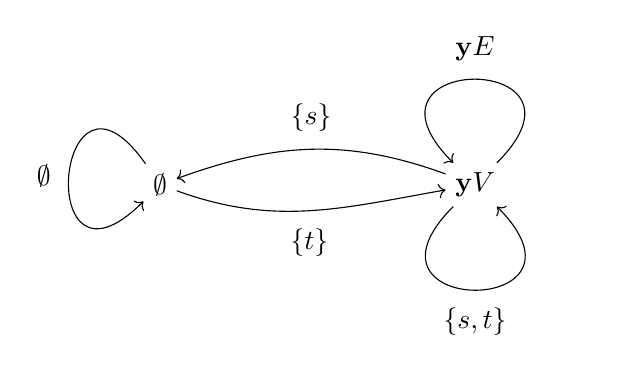
\begin{tikzpicture}
 \node (x) at (-2,0) {$\emptyset$};
 \node (y) at ( 2,0) {$\mathbf{y}V$};
 \path (x) edge [out=125, in=225, looseness=0.8, loop, distance=2cm, ->] node[left= 3pt] {$\emptyset$} (x);
 \path (y) edge [out= 45, in=135, looseness=0.8, loop, distance=2cm, ->] node[above=3pt] {$\mathbf{y}E$} (y);
 \path (y) edge [out=225, in=315, looseness=0.8, loop, distance=2cm, ->] node[below=3pt] {$\{s,t\}$} (y);
 \path (x) edge [out=340, in=190, ->] node[below=3pt] {$\{t\}$} (y);
 \path (y) edge [out=160, in=20, ->] node[above=3pt] {$\{s\}$} (x);
\end{tikzpicture}
\caption{The subobject classifier of $\mathscr{E}$}
\label{fig:subobject classifier for graph topos}
\end{figure}

The subobject classifier is thus given by
\[ \text{true} : 1 \to \Omega, \qquad v \mapsto \mathbf{y}V, \; e \mapsto \mathbf{y}E. \]
% If $X \in \mathscr{E}$ and $S \subseteq X$ a subgraph, then the classifying map $\chi_S : X \to \Omega$ works as follows:
% \begin{itemize}
% 	\item For each vertex $v \in X(V)$:
% 	\begin{itemize}
% 		\item If $v \not\in S(V)$, then $\chi_S(V)(v) = \emptyset$.
% 		\item If $v \in S(V)$, then $\chi_S(V)(v) = \mathbf{y}V$.
% 	\end{itemize}
% 	\item For each edge $e \in X(E)$:
% 	\begin{itemize}
% 		\item If $e \in S(E)$, then $\chi_S(E)(e) = \mathbf{y}E$.
% 		\item Else (we know that $e \not\in S(E)$):
% 		\begin{itemize}
% 			\item If $X(s)(e), X(t)(e) \in S(V)$, then $\chi_S(E)(e) = \{s,t\}$ (the edge is not in $S$, but both its source and target vertices are).
% 			\item Else if $X(s)(e) \in S(V)$, $X(t)(e) \not\in S(V)$, then $\chi_S(E)(e) = \{s\}$ (the edge is not in $S$, and only its source vertex is in $S$).
% 			\item Else if $X(s)(e) \not\in S(V)$ $X(t)(e) \in S(V)$, then $\chi_S(E)(e) = \{t\}$ (the edge is not in $S$, and only its target vertex is in $S$).
% 			\item Else $\chi_S(E)(e) = \emptyset$.
% 		\end{itemize}
% 	\end{itemize}
% \end{itemize}
% Basically, this works as you'd expect for subgraphs in a picture. You can leave out edges in a subgraph, but keep some of its target and source vertices.
% The negation operator $\neg : \Omega \to \Omega$ is a natural transformation with two components $\neg_V : \Omega V \to \Omega V$ and $\neg_E : \Omega E \to \Omega E$. They are defined as (cf. page 56 of Maclane\&Moerdijk)
% \[ \neg_V : \Omega V \to \Omega V, \qquad \neg_V(\emptyset) = \mathbf{y}V, \; \neg_V(\mathbf{y}V) = \emptyset, \]
% and
% \[ \neg_E : \Omega E \to \Omega E, \]
% explicitly calculated as
% \begin{align*}
% \neg_E(\emptyset) &= \mathbf{y}E, \\
% \neg_E(\mathbf{y}E) &= \emptyset, \\
% \neg_E(\{s\}) &= \emptyset\\
% \neg_E(\{t\}) &= \emptyset\\
% \neg_E(\{s,t\}) &= \emptyset\\
% \end{align*}
Now let $\mathscr{E}_{\lcf}$ be the Boolean topos of locally constant objects of $\mathscr{E}$. Since $\mathscr{E}_{\lcf}$ is Boolean, its subobject classifier is given by
\[ \Omega_{\lcf} = 1 + 1 \]
generated by the morphisms
\[ \text{true} : 1 \to \Omega, \qquad \text{false} = \neg \circ \text{true} : 1 \to \Omega. \]
So the graph $\Omega_{\lcf}$ looks like Figure \ref{fig:subobject classifier for lcf graph topos}.

\begin{figure}
\centering
\begin{tikzpicture}
 \node (x) at (-2,0) {$\emptyset$};
 \node (y) at ( 2,0) {$\mathbf{y}V$};
 \path (x) edge [out=125, in=225, looseness=0.8, loop, distance=2cm, ->] node[left= 3pt] {$\emptyset$} (x);
 \path (y) edge [out= 45, in=135, looseness=0.8, loop, distance=2cm, ->] node[above=3pt] {$\mathbf{y}E$} (y);
\end{tikzpicture}
\caption{The subobject classifier of $\mathscr{E}_{\lcf}$}
\label{fig:subobject classifier for lcf graph topos}
\end{figure}

Let $C_n$ be a cyclic graph with $n$ vertices and $n$ edges, $n > 0$. Then $C_n$ is locally constant finite; take $U$ to be the connected graph with $n$ vertices and $n-1$ edges. The product $C_n \times U$ is then a disjoint union of $n$ copies of $U$, so that we have an isomorphism $C_n \times U \cong \Delta(n) \times U$, where $\Delta(n)$ are $n$ copies of the graph with $1$ vertex and $1$ edge. Moreover, this isomorphism respects the projection down to $U$, so that $C_n$ is locally constant finite as per \cref{def:locally constant finite}.

I claim that disjoint unions of the $C_n$ are the only type of objects in $\mathscr{E}_{\lcf}$. Indeed, by \cref{prop:locally constant iff every restriction map is a bijection}, the restriction maps of an object $X \in \mathscr{E}_{\lcf}$ must be constant. This just translates to the fact that there are as many vertices as there are edges.

Moreover, each $C_n$ is an atom in $\mathscr{E}_{\lcf}$. Indeed, from the definition of $\Omega_{\lcf}$ we find that removing an edge means that we are forced to remove the vertices that the edge was attached to, too (this need not happen in $\mathscr{E}$). Thus $C_n$ has no subobjects other than the empty graph.

Next, we claim that every $C_n$ is also a Galois object. Indeed, there is a $\Z/n\Z$ action on the edges of $C_n$; simply cyclic shift the edges. Clearly then $\Aut(C_n) \cong C_n(E)$.
% Thus we may conclude that
% \begin{claim}
% Let $\mathbf{G}$ be the full subcategory of $\mathbf{I}$ whose objects are Galois. Then every object of $\mathbf{G}$ is of the form $(C_n,e)$ for some $n > 0$.
% \end{claim}
% \begin{proof}
% Write $C_n(V) = \{v_0,\ldots,v_{n-1}\}$ and $C_n(E) = \{e_0,\ldots,e_{n-1}\}$. Then $\Aut(C_n) = \Z/n\Z$, with action given by $m \cdot e_j = e_{j + m \bmod{n}}$. Hence $\Aut(C_n) \cong p^*(C_n)$, so $\mathbf{G}$ certainly contains all the $(C_n,e)$. Conversely suppose that $(A,e) \in \mathbf{G}$. Let $\varphi : A \times U \to \Delta n \times U$ be an isomorphism over $U$, where $U \to 1$ has global support. Note that $\# A = \# \Delta n = n$. Let $v \in A$ be a vertex. Let $\partial^+(v)$ be the number of incoming edges into the vertex $v$. Assume that $\partial^+(v) = 0$. Then for all $(v,u) \in A \times U$ we also have $\partial^+(v,u) = 0$. However $\varphi(v,u) = (v_j,u)$ for some $v_j \in C_n$, and $\partial^+(v_j,u) > 0$ for some $u \in U(V)$. This is in contradiction with $\partial^+(v,u) = 0$ for all $u \in U(V)$. So we conclude that $\partial^+(v) > 0$ for all $v \in A(V)$. This forces $\partial^+(v) = 1$ for all $v \in A(V)$, because $n = \sum_{v \in A(V)} \partial^+(v)$. Since we didn't use the fact that these edges are incoming, the same argument shows that the number of outgoing edges is also $1$ for each $v \in A(V)$. Finally, since $A$ is connected we may conclude that $A = C_n$.
% \end{proof}
% So the cycles form a cofinal subcategory of $\mathbf{I}$. 
Thus we may conclude that
\[ \pi_1(\mathscr{E}, E) = \lim_{\leftarrow n} \Aut(C_n) \cong \lim_{\leftarrow n} \Z/n\Z = \widehat{\Z}. \]
It is to be noted that if we chose a different point of $\mathscr{E}$, say the object $V$, using \cref{constr:how to get points}, we would end up with the same argumentation; there's a  $\Z/n\Z$ action on the vertices, and it can only be a $\Z/n\Z$ action because the source and target vertices of the edges of $C_n$ must match up.

% \section{Worked Example}

% Take a 

% An $n$-simplex $\sigma$ of a simplicial set $S$ is called \emph{degenerate} if there exists an $m < n$ and an order-preserving surjection $f : \mathbf{n} \to \mathbf{m}$ and an $m$-simplex $\tau$ of $S$ such that $\sigma = (Sf)(\tau)$. Note that $0$-simplices (vertices) are never degenerate. An $n$-simplex $\sigma$ is called \emph{non-degenerate} if it is not degenerate.

% \begin{lemma}[Eilenberg-Zilber]
% \label{lem:eilenberg-zilber} Let $S \in \mathbf{SSets}$. For each $n$-simplex $\sigma \in S_n$ there exists a unique order-preserving surjection $f : \mathbf{n} \to \mathbf{m}$ and a unique non-degenerate $m$-simplex $\tau \in S_m$ such that $\sigma = (Sf)(\tau)$.
% \end{lemma}
% \begin{proof}
% \begin{color}{red} Put a reference here... \end{color}
% If $\sigma$ is already non-degenerate, take $m=n$ and $f = \id$. If $\sigma$ is degenerate, then there exists some surjection $f_1 : [n] \to [m_1]$ with $m_1 < n$ and an $m_1$-simplex $\sigma_1$ such that $\sigma = (Sf_1)(\sigma_1)$. If $\sigma_1$ is non-degenerate, we are done. Otherwise, continue in this way until we reach a $\sigma_j$ that is non-degenerate. This process ends eventually since with each iteration, $m_i < m_{i-1}$, and vertices are always non-degenerate.
% So the existence of such a pair $(f,\tau)$ with $\sigma = (Sf)(\tau)$ is established. Suppose then that $(f',\tau')$ is another pair with $\sigma = (Sf')(\tau')$. Consider the pushout
% \[ \begin{tikzcd}
% \left[n\right] \arrow{r}{f} \arrow[swap]{d}{f'} & \left[m\right] \arrow{d}{\pi} \\
% \left[m'\right] \arrow[swap]{r}{\pi'} & \left[p\right]
% \end{tikzcd} \]
% in $\mathbf{\Delta}$. We can apply the Yoneda functor to get a commutative diagram
% \[ \begin{tikzcd}
% \mathbf{\Delta}\left(-,\left[n\right]\right) \arrow{r}{\mathbf{\Delta}\left(-,f\right)} \arrow[swap]{d}{\mathbf{\Delta}\left(-,f'\right)} & \mathbf{\Delta}\left(-,\left[m\right]\right) \arrow{d}{\mathbf{\Delta}\left(-,\pi\right)} \\
% \mathbf{\Delta}\left(-,\left[m'\right]\right) \arrow[swap]{r}{\mathbf{\Delta}\left(-,\pi'\right)} & \mathbf{\Delta}\left(-,\left[p\right]\right)
% \end{tikzcd} \]
% in $\mathbf{SSet}$. This diagram is still a pushout. While the $n$-simplex $\sigma$ is an element of the set $S_n$, it may equivalently be regarded as a functor $\sigma : \mathbf{\Delta}(-,[n]) \to S$ describing how the simplex is laid into the simplicial set. Similarly for $\tau$ and $\tau'$. Hence we have a commutative diagram
% \[ \begin{tikzcd}
% \mathbf{\Delta}\left(-,\left[n\right]\right) \arrow{r}{\mathbf{\Delta}\left(-,f\right)} \arrow[swap]{d}{\mathbf{\Delta}\left(-,f'\right)} & \mathbf{\Delta}\left(-,\left[m\right]\right) \arrow{d}{\mathbf{\Delta}\left(-,\pi\right)} \arrow[bend left]{ddr}{\tau} \\
% \mathbf{\Delta}\left(-,\left[m'\right]\right) \arrow[swap]{r}{\mathbf{\Delta}\left(-,\pi'\right)} \arrow[swap, bend right]{rrd}{\tau'} & \mathbf{\Delta}\left(-,\left[p\right]\right) \arrow[dotted]{dr}{\exists ! \rho} \\
% \; & \; & S
% \end{tikzcd} \]
% Since $\tau \circ \mathbf{\Delta}(-,f) = \sigma = \tau' \circ\mathbf{\Delta}(-,f')$, there exists a unique mediating $\rho$ such that $\mathbf{\Delta}(-,\pi) \circ \rho = \tau$ and $\mathbf{\Delta}(-,\pi') \circ \rho = \tau'$ as indicated by the dotted arrow. We can regard $\rho$ equivalently as a $p$-simplex in the set $S_p$, while $\pi$ and $\pi'$ are order-preserving surjections. So we see that $\tau = (S \pi)(\rho)$ and $\tau' = (S \pi')(\rho)$. But $\tau$ and $\tau'$ are both non-degenerate. So we must have $\pi = \pi' = \id$, $m=p=m'$, and hence $\tau = \tau'$.
% \end{proof}




	%!TEX root = main.tex
%
% simplicialcomplexes.tex
%

\chapter{Simplicial Sets}

In this preliminary section we touch upon some concepts regarding simplicial complexes. In some way they are just a special case of a presheaf topos. On the other hand, they have some intrinsic properties not found in other presheaf toposes. Most of this section is from \cite{goersjardinne09} and \cite{JT2008}. The aim of this section is to define the notion of a star, the nerve of a category and the geometric realization.

\section{Basic Definitions}

\begin{definition}
\label{def: finite cardinal}
Let $n \geq 0$ be a natural number. By the boldface $\mathbf{n}$ we mean the \emph{category} consisting of precisely $n+1$ objects, denoted by $0,1,2,\ldots,n-1,n$, and whose morphisms are precisely
\[ 0 \to 1 \to \cdots \to (n-1) \to n. \]
so that $\mathbf{n}$ may be regarded as a totally ordered set.
\end{definition}

\begin{definition}
\label{def:order category}
By $\mathbf{\Delta}$ we mean the category whose objects are the $\mathbf{n}$'s and whose morphisms are functors $\theta : \mathbf{n} \to \mathbf{m}$.
\end{definition}
If $\theta : \bf{n} \to \bf{m}$ is a morphism in $\bf{\Delta}$, we can also view it as an order-preserving function on the totally ordered sets $\bf{n}$ and $\bf{m}$. It is fruitful to confuse the two viewpoints sometimes.
Among the morphisms in $\mathbf{\Delta}$ are two special types, namely the coface and codegeneracy maps.
\begin{definition}
\index{coface map}
\index{codegeneracy map}
\label{def:coface and codegeneracy maps}
Let $\bf{n} \in \bf{\Delta}$ and let $j \in \bf{n}$. The $j$'th \emph{coface} map is the morphism
\[ d^j : \bf{n-1} \to \bf{n} \]
defined by
\[ d^j\left(0 \to \cdots \to (n-1) \right) = 0 \to \cdots \to (j-1) \to (j+1) \to \cdots \to (n+1), \]
i.e., ``skip $j$'', and the $j$'th \emph{codegeneracy} map is the morphism
\[ s^j : \bf{n+1} \to \bf{n} \]
defined by
\[ s^j\left(0 \to \cdots \to (n+1) \right) = 0 \to \cdots \to (j-1) \to j \to j \to (j+1) \to \cdots \to n, \]
i.e., ``repeat $j$''.
\end{definition}
If $\theta : \bf{n} \to \bf{m}$ is an order-preserving map, one can decompose it uniquely into a composite $\theta = \alpha \circ \beta$ where $\beta : \bf{n} \to \bf{p}$ is surjective and $\alpha : \bf{p} \to \bf{m}$ is injective. Then $\beta$ may be decomposed into a bunch of codegeneracy maps and $\alpha$ may be decomposed into a bunch of coface maps. So the morphisms in $\bf{\Delta}$ are generated by the coface and codegeneracy maps. Moreover, we have
\begin{lemma}[The Cosimplicial Identities]
\index{cosimplicial identities}
\label{lem:cosimplicial identities}
Let $n \geq 2$. Consider the diagram
\[ \begin{tikzcd}
\bf{n} \arrow[shift left=0.2em]{r}{s^j} \arrow[shift left=0.2em]{d}{s^i} & \bf{n-1} \arrow[shift left=0.2em]{l}{d^j} \arrow[shift left=0.2em]{d}{s^i} \\
\bf{n-1} \arrow[shift left=0.2em]{u}{d^i} \arrow[shift left=0.2em]{r}{s^{j-1}} & \bf{n-2} \arrow[shift left=0.2em]{u}{d^i} \arrow[shift left=0.2em]{l}{d^{j-1}}
\end{tikzcd} \]
in $\bf{\Delta}$. Then
\begin{align*}
d^j d^i &= d^i d^{j-1} & \forall \; i < j \\
s^{j-1} s^i &= s^i s^j & \forall \; i < j \\
s^j d^i &= d^i s^{j-1} & \forall \; i < j \\
s^i d^i &= \id & \; \\
s^i d^j &= d^{j-1} s^i & \forall \; i < j-1 \\
s^i d^{i+1} &= \id & i=j-1
\end{align*}
Moreover, the square of $s$'s is an absolute pushout, and the square of $d$'s is an absolute pullback.
\end{lemma}
\begin{proof}
The proof is easy. It's just a lot of bookkeeping.
\end{proof}
Recall that a (co)limit is termed absolute when it is preserved by \emph{any} functor. Since every morphism $\theta : \bf{n} \to \bf{m}$ factors uniquely into a composite of coface and codegeneracy maps, we conclude from the previous lemma
\begin{theorem}
\label{thm:absolute colimits and limits in the order category}
The category $\bf{\Delta}$ has absolute pushouts of surjections and absolute non-empty intersections of injections.
\end{theorem}

\begin{definition}
\index{standard $n$-simplex}
The category of \emph{simplicial sets} $\bf{S}$ is defined to be $\mathbf{Set}^{\bf{\Delta}^{op}}$.
\end{definition}
In practice, a simplicial set $X \in \bf{S}$ is determined when for each natural number $n$ a set $X_n$ is given together with face maps $d_i : X_{n+1} \to X_{n}$ and degeneracy maps $s_i : X_{n-1} \to X_{n}$.

\begin{definition}
The \emph{standard $n$-simplex} is the simplicial set $\Hom_{\Delta}(-,\bf{n}) = \bf{\Delta}(-,\bf{n}) = \bf{y}\bf{n}$.
\end{definition}

By a standard application of Yoneda's lemma we immediately obtain

\begin{lemma}
Let $X \in \bf{S}$ be a simplicial set. Then for each natural number $n \geq 0$ we have
\[ X_n \cong \Hom_{\mathbf{S}}\left( \mathbf{\Delta}(-,\mathbf{n}) , X \right). \]
\end{lemma}

\begin{definition}
\index{degenerate simplex}
\index{non-degenerate simplex}
An $n$-simplex $\sigma \in X_n$ is called \emph{degenerate} if there is a surjection $f : \mathbf{n} \to \mathbf{m}$ with $m < n$ and an $m$-simplex $\tau \in X_m$ such that $\sigma = X(f)(\tau)$. A simplex is called \emph{non-degenerate} if it is not degenerate.
\end{definition}

A very useful lemma which we shall use over and over again is the following.

\begin{lemma}[Eilenberg-Zilber]
\label{lem:eilenberg-zilber}
For each $n$-simplex $\sigma \in X_n$ there exists a unique order-preserving surjection $f : \mathbf{n} \to \mathbf{m}$ and a unique non-degenerate $m$-simplex $\tau \in X_m$ such that $\sigma = X(f)(\tau)$.
\end{lemma}
\begin{proof}
We follow \cite[Proposition 1.2.2]{JT2008}.
If $\sigma$ is already non-degenerate, take $m=n$ and $f = \id$. If $\sigma$ is degenerate, then there exists some surjection $f_1 : \mathbf{n} \to \mathbf{m}_1$ with $m_1 < n$ and an $m_1$-simplex $\sigma_1$ such that $\sigma = X(f_1)(\sigma_1)$. If $\sigma_1$ is non-degenerate, we are done. Otherwise, continue in this way until we reach a $\sigma_j$ that is non-degenerate. This process ends eventually since with each iteration, $m_i < m_{i-1}$, and vertices are always non-degenerate.
So the existence of such a pair $(f,\tau)$ with $\sigma = X(f)(\tau)$ is established. Suppose then that $(f',\tau')$ is another pair with $\sigma = X(f')(\tau')$. Consider the pushout
\[ \begin{tikzcd}
\mathbf{n} \arrow{r}{f} \arrow[swap]{d}{f'} & \mathbf{m} \arrow{d}{\pi} \\
\mathbf{m}' \arrow[swap]{r}{\pi'} & \mathbf{p}
\end{tikzcd} \]
in $\mathbf{\Delta}$. We can apply the Yoneda functor to get a commutative diagram
\[ \begin{tikzcd}
\mathbf{\Delta}\left(-,\mathbf{n}\right) \arrow{r}{\mathbf{\Delta}\left(-,f\right)} \arrow[swap]{d}{\mathbf{\Delta}\left(-,f'\right)} & \mathbf{\Delta}\left(-,\mathbf{m}\right) \arrow{d}{\mathbf{\Delta}\left(-,\pi\right)} \\
\mathbf{\Delta}\left(-,\mathbf{m}'\right) \arrow[swap]{r}{\mathbf{\Delta}\left(-,\pi'\right)} & \mathbf{\Delta}\left(-,\mathbf{p}\right)
\end{tikzcd} \]
in $\mathbf{S}$. This diagram is still a pushout by \cref{thm:absolute colimits and limits in the order category}. While the $n$-simplex $\sigma$ is an element of the set $X_n$, it may equivalently be regarded as a functor $\sigma : \mathbf{\Delta}(-,\mathbf{n}) \to S$ describing how the simplex is laid into the simplicial set. Similarly for $\tau$ and $\tau'$. Hence we have a commutative diagram
\[ \begin{tikzcd}
\mathbf{\Delta}\left(-,\mathbf{n}\right) \arrow{r}{\mathbf{\Delta}\left(-,f\right)} \arrow[swap]{d}{\mathbf{\Delta}\left(-,f'\right)} & \mathbf{\Delta}\left(-,\mathbf{m}\right) \arrow{d}{\mathbf{\Delta}\left(-,\pi\right)} \arrow[bend left]{ddr}{\tau} \\
\mathbf{\Delta}\left(-,\mathbf{m}'\right) \arrow[swap]{r}{\mathbf{\Delta}\left(-,\pi'\right)} \arrow[swap, bend right]{rrd}{\tau'} & \mathbf{\Delta}\left(-,\mathbf{p}\right) \arrow[dotted]{dr}{\exists ! \rho} \\
\; & \; & S
\end{tikzcd} \]
Since $\tau \circ \mathbf{\Delta}(-,f) = \sigma = \tau' \circ\mathbf{\Delta}(-,f')$, there exists a unique mediating $\rho$ such that $\mathbf{\Delta}(-,\pi) \circ \rho = \tau$ and $\mathbf{\Delta}(-,\pi') \circ \rho = \tau'$ as indicated by the dotted arrow. 
We can regard $\rho$ equivalently as a $p$-simplex in the set $X_p$, while $\pi$ and $\pi'$ are order-preserving surjections. So we see that $\tau = X(\pi)(\rho)$ and $\tau' = X(\pi')(\rho)$. But $\tau$ and $\tau'$ are both non-degenerate. So we must have $\pi = \pi' = \id$, $m=p=m'$, and hence $\tau = \tau'$.
\end{proof}

Recall that every presheaf is a colimit of representable presheaves by \cref{prop:every presheaf is a colimit of representables}. The good news is that there are not many different representable presheaves in $\bf{S}$. So we conclude

\begin{lemma}
\label{lem:every simplicial set is a colimit of standard n simplices}
If $X \in \bf{S}$ is a simplicial set, there is a canonical isomorphism
\[ X \cong \colim \left( \int_{\mathbf{\Delta}} X \xrightarrow{\pi_X} \mathbf{\Delta} \xrightarrow{\mathbf{y}} \mathbf{Set}^{\mathbf{\Delta}^{op}} \right) \]
\end{lemma}
The above lemma tells you ``how the standard simplices comprise $X$'', and is very combinatorial in nature. It's often convenient to view \cref{lem:every simplicial set is a colimit of standard n simplices} as a different (but equivalent, of course) colimit. Namely, define $\mathbf{\Delta}  \downarrow  X$ to be the category whose objects are maps $\sigma : \mathbf{\Delta}(-,\mathbf{n}) \to X$ (or just simplices of $X$). An arrow in $\mathbf{\Delta}  \downarrow  X$ is a commutative diagram of simplicial maps
\[ \begin{tikzcd}
\mathbf{\Delta}(-,\mathbf{n}) \arrow[swap]{dd}{\theta} \arrow{dr}{\sigma} & \; \\
 & X \\
\mathbf{\Delta}(-,\mathbf{m}) \arrow[swap]{ur}{\tau} & \;
\end{tikzcd} \]
It is not hard to prove that the colimit in \cref{lem:every simplicial set is a colimit of standard n simplices} is the same thing as
\begin{lemma}
\[ X \cong \colim_{\stackrel{\mathbf{\Delta}(-,\mathbf{n}) \to X}{\text{in } \mathbf{\Delta}\downarrow X}} \mathbf{\Delta}(-,\mathbf{n}). \]
\end{lemma}

\section{Geometric Realization}

\begin{definition}
\index{standard geometric $n$-simplex}
\label{def:standard geometric n-simplex}
The \emph{standard geometric $n$-simplex} is the topological space
\[ \Delta^n := \left\{ (t_0,\ldots,t_n) \in \R^{n+1} \mid \sum_{i=0}^n t_i = 1,\; t_i \geq 0 \text{ for all } i \right\} \]
endowed with the subspace topology from the metric space $\R^{n+1}$.
\end{definition}
There is a functor $|-| : \mathbf{\Delta} \to \mathbf{Top}$ defined by sending $\bf{n}$ to the standard geometric $n$-simplex in $\R^{n+1}$. It's easy to visualize what $|-|$ should do with the coface and codegeneracy maps.
As with all such constructions, once we have a way to turn representable objects into an object of interest in a category, we have a way to turn every presheaf into an object of interest in a category. For a more precise meaning of the previous sentence, we have the following definition.
\begin{definition}
\index{geometric realization}
\label{def:geometric realization of a simplicial set}
The \emph{geometric realization} of $X$ is defined to be the colimit of spaces
\[ |X| := \colim_{\stackrel{\mathbf{\Delta}(-,\mathbf{n}) \to X}{\text{in } \mathbf{\Delta}\downarrow X}} \Delta^n \in \mathbf{Top} \]
\end{definition}
Elements of $|X|$ are equivalence classes of pairs $[\sigma, t]$, where $\sigma \in X_n$ is an $n$-simplex and $t \in \Delta^n$. The equivalence relation is defined by the rule
\[ \left(X(\theta)(\sigma), t \right) \sim \left( \sigma, |\theta|(t) \right), \qquad \theta : \mathbf{n} \to \mathbf{m}. \]
In fact, this is reminiscent of the tensor product! Unfortunately, $\mathbf{Top}$ is not a topos. Moreover, $|X|$ is a space, not just a set (as it is for the tensor product). So we cannot formally define the geometric realization in this way.
A map $f : X \to Y$ of simplicial sets (so, a natural transformation between the presheaves) determines a functor
\[ \mathbf{\Delta} \downarrow f : \mathbf{\Delta} \downarrow X \to \mathbf{\Delta} \downarrow Y, \qquad \sigma \mapsto f \circ \sigma. \]
So we get a continuous map
\[ |f| : |X| \to |Y|, \qquad [\sigma,t] \mapsto [f \circ \sigma, t]. \]
Hence $|-| : \mathbf{\Delta} \to \mathbf{Top}$ extends to a functor $|-| : \mathbf{S} \to \mathbf{Top}$. There's also a functor going the other way. Observe that for any given topological space $S \in \mathbf{Top}$ we have a simplicial set $\Sing(S)$ defined on objects by $\Sing(S)_n := \Hom_{\mathbf{Top}}\left(\Delta^n, S\right)$. It's an exercise to determine what $\Sing$ should do with continuous maps, and what the face and degeneracy maps are for $\Sing(S)$.

\begin{theorem}
The functor $|-|$ is the left-adjoint of $\Sing$.
\end{theorem}
\begin{proof}
There are natural bijections
\begin{align*}
\Hom_{\mathbf{Top}}\left(|X|, S \right) &= \Hom_{\mathbf{Top}}\left( \colim_{\stackrel{\mathbf{\Delta}(-,\mathbf{n}) \to X}{\text{in } \mathbf{\Delta}\downarrow X}} \Delta^n, S \right) \\
&\cong \lim_{\stackrel{\mathbf{\Delta}(-,\mathbf{n}) \to X}{\text{in } \mathbf{\Delta}\downarrow X}} \Hom_{\mathbf{Top}}\left( \Delta^n, S \right) \\
&\cong \lim_{\stackrel{\mathbf{\Delta}(-,\mathbf{n}) \to X}{\text{in } \mathbf{\Delta}\downarrow X}} \Hom_{\mathbf{S}}\left( \mathbf{\Delta}(-,\mathbf{n}), \Sing(S) \right) \\
&\cong \Hom_{\mathbf{S}}\left(X, \Sing(S) \right).
\end{align*}
\end{proof}

\section{The Nerve of a Category}
From the way we defined the category $\mathbf{\Delta}$ we have an obvious inclusion functor
\[ \mathbf{\Delta} \to \mathbf{Cat}, \qquad \mathbf{n} \mapsto \mathbf{n}. \]
So we have a way to change representable objects into objects of a category that we are interested in. We can do the whole construction again, but this time in $\mathbf{Cat}$ instead of $\mathbf{Top}$. It's possible to set up an adjoint pair of functors between $\mathbf{S}$ and $\mathbf{Cat}$ just like for the adjoint pair $|-| \dashv \Sing$. We will not be needing the left adjoint. What we will be needing from this adjunction, though, is the right adjoint. We define formally
\begin{definition}
\index{nerve}
\label{def:nerve of a category}
Let $\mathbf{C} \in \mathbf{Cat}$ be a small category. We define the \emph{nerve} of $\mathbf{C}$ to be the simplicial set $N\mathbf{C}$ defined for each natural number $n \geq 0$ as the set
\[ (N\mathbf{C})_n := \Hom_{\mathbf{Cat}}\left(\mathbf{n}, \mathbf{C} \right). \]
\end{definition}
Spelled out in detail, this means that the $0$-simplices are the objects of $\mathbf{C}$ (which is indeed a set). If $n>0$, then an $n$-simplex of $(N\mathbf{C})_n$ is an $n$-tuple
\[ A_0 \xrightarrow{f_1} A_1 \xrightarrow{f_2} \cdots \xrightarrow{f_n} A_n \]
of composable morphisms $f_i : A_{i-1} \to A_i$. We'll denote such simplices more compactly by $(f_1,\ldots,f_n)$. The face maps
\[ d_j : (N\mathbf{C})_{n} \to (N\mathbf{C})_{n-1} \] compose two consecutive morphisms at the $j$'th position to get an $(n-1)$-tuple of composable morphisms when $0 < j < n$, and they discard the outer morphism when $j = 0$ or $n$. The degeneracy maps
\[ s_j : (N\mathbf{C})_n \to (N \mathbf{C})_{n+1} \]
insert an identity morphism at the $j$'th position to get a degenerate $(n+1)$-tuple.

\section{Star Neighborhoods}

From this point on, the thesis consists of mostly original work, so the proofs become more detailed.

\begin{lemma}
\label{lem:subcomplex is closed subset in the realization}
Let $S \in \mathbf{S}$ be a simplicial complex and $T \subset S$ a subcomplex. Then $|T| \subset |S|$ is a closed set.
\end{lemma}
\begin{proof}
Let $\sigma \in S_n$ be an $n$-simplex of $S$. Let $I$ be the set of all possible faces of $\sigma$ which are contained in $T$. Note that $I$ is a finite set. Therefore $\bigcup_{\tau \in I}|\tau|$ is closed in $|\sigma|$.
\end{proof}

\begin{definition}
\index{star}
\label{def:star of a simplex}
Let $S \in \mathbf{S}$ be a simplicial set, and an $n$-simplex $\sigma \in S_n$. The \emph{star} of $\sigma$, denoted $\st(\sigma)$, is the set of all simplices in $S$ which contain $\sigma$ as an eventual face.
\end{definition}

This means that $\sigma \in S_n$ is an eventual face of some $\tau \in S_m$ with $m>n$ if and only if there exist natural numbers $i_1,i_2,\ldots,i_{m-n}$ such that $\sigma = (d_{i_{m-n}} \circ \cdots \circ d_{i_{2}} \circ d_{i_{1}})(\tau)$. If $m=n$, then $\sigma$ is a face of $\sigma$, so $\sigma \in \st(\sigma)$. If $m < n$, then $S_m \cap \st(\sigma) = \emptyset$. Put in a more functorial way, identify $\sigma$ and $\tau$ as functors $\sigma : \mathbf{\Delta}(-,\mathbf{n}) \to S$ and $\tau : \mathbf{\Delta}(-,\mathbf{m}) \to S$. Then $\sigma$ is an eventual face of $\tau$ if and only if there exists an injective order-preserving map $\theta : \mathbf{n} \to \mathbf{m}$ such that
\begin{equation}
\label{eq:sigma is eventual face of tau diagram}
\begin{tikzcd}
\mathbf{\Delta}(-,\mathbf{n}) \arrow{dr}{\sigma} \arrow[swap]{dd}{\mathbf{\Delta}(-,\theta)} & \\
& S \\
\mathbf{\Delta}(-,\mathbf{m}) \arrow[swap]{ur}{\tau}
\end{tikzcd}
\end{equation}
is a commutative diagram of simplicial sets.

\begin{definition}
\label{def:simplicial set minus a simplex}
Let $S \in \mathbf{S}$ and take an $n$-simplex $\sigma \in S_n$. The simplicial set $S - \sigma$ is defined as follows. For any $n \in \N$, we set
\[ (S-\sigma)_n := \left\{ \tau \in S_n : \tau \not\in \st(\sigma) \right\}. \]
The face and degeneracy maps for $S-\sigma$ are the same as from $S$, and by definition of the star they are well-defined.
\end{definition}

It is obvious that $S - \sigma \subset S$. As a consequence, $|S-\sigma|$ is a closed subspace inside $|S|$ by \cref{lem:subcomplex is closed subset in the realization}.

\begin{definition}
\index{realization of the star}
\label{def:realization of the star}
Let $S \in \mathbf{S}$ be a simplicial set and $\sigma \in S_n$ an $n$-simplex. We define the \emph{realization of the star} $\sigma^* \subset |S|$ as the open subspace $|S| - |S-\sigma|$.
\end{definition}
Observe that if $v \in S_0$ is a $0$-simplex (a vertex), then the only point $p \in v^*$ with the property that $p = |w|$ for some $w \in S_0$ is $v$.

% \begin{definition}
% Let $S \in \mathbf{S}$ be a simplicial set and take a non-degenerate $n$-simplex $\sigma \in S_n$. Identify $|\sigma|$ with its continuous map $\sigma : \Delta^n \to |S|$. Because $\sigma$ is non-degenerate, the map $|\sigma|$ is injective. We define the \emph{interior} of $\sigma$ as the image of $\{(t_0,\ldots,t_n) \in \Delta^n : t_i > 0\}$, denoted by $\Int(\sigma)$. If $\sigma$ is degenerate, there exists a unique non-degenerate $m$-simplex $\tau$ and a surjective order-preserving map $f : [n] \to [m]$ such that $f^* \tau = \sigma$. In particular, $|\tau|$ and $|\sigma|$ give the same realization in $|S|$. We define the \emph{interior} of the degenerate $n$-simplex $\sigma$ as the interior of the non-degenerate $m$-simplex $\tau$.
% \end{definition}

\begin{definition}
\index{interior}
\label{def:interior of a simplex}
Let $S \in \mathbf{S}$ be a simplicial set and take an $n$-simplex $\sigma \in S_n$. Identify the realization of $\sigma$ in $|S|$ with its continuous map $|\sigma| : \Delta^n \to |S|$. We define the \emph{interior} of $\sigma$ as the image of $\{(t_0,\ldots,t_n) \in \Delta^n : t_i > 0,\; i=0,\ldots,n\}$.
\end{definition}

Observe that this definition works fine even for degenerate simplices, and note also that the interior of a $0$-simplex is a point in $|S|$. Note also that the interior of a simplex is not necessarily open in $|S|$. However, we do have

\begin{lemma}
\label{lem:realization of the star is union of the interiors}
Let $\sigma \in S_n$ be an $n$-simplex of a simplicial set $S \in \mathbf{S}$. Then $\sigma^* = \bigcup_{\tau \in \st(\sigma)} \Int(\tau)$.
\end{lemma}
\begin{proof}
The inclusion $\bigcup_{\tau \in \st(\sigma)} \Int(\tau) \subseteq \sigma^*$ is trivial. Let us prove the other inclusion.

Let $p \in \sigma^*$. Then $p \not\in |S-\sigma|$. This means that $p$ is not in the (closed) image of any $m$-simplex $|\tau| : \Delta^m \to |S|$ for which $\sigma$ is \emph{not} an eventual face. 
But $p \in |S|$, so what remains is that $p$ is in the image of an $m$-simplex $|\tau| : \Delta^m \to |S|$ for which $\sigma$ is an eventual face. 
By \cref{lem:eilenberg-zilber}, we may assume $\tau$ to be non-degenerate. 
Let $(t_0,\ldots,t_m) \in \Delta^m$ be the barycentric coordinates such that $|\tau|(t_0,\ldots,t_m) = p$. 
If $m=0$ then we are done, so assume $m>0$. If $t_i = 0$ for some $i$, we may replace $\tau$ by its face $d_i \tau$ and replace the barycentric coordinates by $(t_0,\ldots,t_{i-1},t_{i+1},\ldots,t_m)$. After such a replacement, we still have $d_i \tau \in \st(\sigma)$. 
Continue in this way until we reach a $k$-simplex $\tau'$, with $k \leq m$, with barycentric coordinates $(t_0,\ldots,t_k)$ with $t_i > 0$ for all $i=0,\ldots,k$. 

\end{proof}

\begin{lemma}
\label{lem:realization of the star is contained in the intersection of the realizations of its faces}
Let $n>0$ and take an $n$-simplex $\sigma \in S_n$ in a simplicial set $S \in \mathbf{S}$. Then
\[ \sigma^* \subset \bigcap_{i=0}^n (d_i \sigma)^*. \]
\end{lemma}
\begin{proof}
If $\tau \in \st(\sigma)$, then $\tau$ is eventually a face of $\sigma$, so it's clearly also eventually a face of $d_i \sigma$ for $i=0,\ldots,n$. Hence $\tau \in \bigcap_{i=0}^n \st(d_i \sigma)$. Therefore $\Int(\tau) \subset (d_i \sigma)^*$ for every $i=0,\ldots,n$.
\end{proof}

\begin{lemma}
\label{lem:realization of the star is connected}
Let $S \in \mathbf{S}$. For every $n$-simplex $\sigma \in S_n$, the realization of the star $\sigma^* \subset |S|$ is a connected subset.
\end{lemma}
\begin{proof}
Suppose that we can write $\sigma^* = U \cup V$, where $U$ and $V$ are two disjoint non-empty open subsets of $\sigma^*$. Let $\tau \in \st(\sigma)$. Then $|\tau|$ is a compact connected metric space, so $\Int(\tau)$ is a connected metric space. but $\Int(\tau) = \left(U \cap \Int(\tau) \right) \cup \left(V \cap \Int(\tau) \right)$, so either $\Int(\tau) \subset U$ or $\Int(\tau) \subset V$. Let $I$ be the set of all $\tau \in \st(\sigma)$ for which $\Int(\tau) \subset U$ and let $J$ be the set of all $\tau \in \st(\sigma)$ for which $\Int(\tau) \subset V$. Both $I$ and $J$ are non-empty. By \cref{lem:realization of the star is union of the interiors}, we find a decomposition
\[ \sigma^* = \bigcup_{\tau \in \st(\sigma)} \Int(\tau) = \bigcup_{\tau \in I} \Int(\tau) \cup \bigcup_{\tau \in J} \Int(\tau). \]
Without loss of generality, $\sigma \in I$. If $\tau \in \st(\sigma)$, with $\tau$ an $m$-simplex, $n \leq m$, then there exists a commutative diagram as in \cref{eq:sigma is eventual face of tau diagram}. Thus, we have a commutative diagram of topological spaces and continuous maps
\[ \begin{tikzcd}
\Delta^n \arrow{dr}{|\sigma|} \arrow[swap]{dd}{|\mathbf{\Delta}(-,\theta)|} & \\
& \left| S \right| \\
\Delta^m \arrow[swap]{ur}{|\tau|}
\end{tikzcd} \]
By connectedness of $\Delta^m$ and $\Delta^n$, we have $\tau \in I$. But this holds for arbitrary $\tau$, so $J$ is empty. A contradiction.
\end{proof}

\begin{lemma}
\label{lem:realizations of stars form an open cover}
The realizations of the stars of vertices form an open cover of $|S|$. That is, $|S| = \bigcup_{v \in S_0} v^*$.
\end{lemma}
\begin{proof}
By \cref{lem:realization of the star is union of the interiors},
\[ \bigcup_{v \in S_0}v^* = \bigcup_{v \in S_0} \bigcup_{\tau \in \st(v)} \Int(\tau). \]
The right-hand-side of this equation exhausts all possible simplices of $S$. So it suffices to prove that every point $p \in |S|$ is contained in the interior of some $n$-simplex $\sigma$.
Let $p \in |S|$. Then $p \in |\sigma|$ for some $n$-simplex $\sigma \in S_n$. By \cref{lem:eilenberg-zilber}, there exists a unique non-degenerate $m$-simplex $\tau \in S_m$ and a surjective order-preserving map $f : \mathbf{n} \to \mathbf{m}$, with $m \leq n$, such that $(Sf)(\tau) = \sigma$. Thus $p \in |\tau|$. If $p \in \Int(\tau)$ then we are done. Otherwise, $p \in |d_i \tau|$ for some $i$. Continue in this way. Eventually this process stops.
\end{proof}


	%!TEX root = main.tex
%
% etalefunctor.tex
%

\chapter{Construction of the McCord Functor}

Let $\mathbf{C} \in \mathbf{Cat}$ be a small category and write $X_\mathbf{C} := |N\mathbf{C}|$. The goal is to find a functor $\mathbf{C} \to \mathbf{LH}/X_\mathbf{C}$, where $\mathbf{LH}$ denotes the category of topological spaces together with local homeomorphisms (etale maps) as morphisms. Recall from \cref{def:LH/X} and \cref{thm:equivalence of categories between etale spaces and sheaves} that $\mathbf{LH}/X_{\mathbf{C}}$ is a Grothendieck topos, and it is connected if and only if $X_{\mathbf{C}}$ is connected, which is the case if and only if $\mathbf{C}$ is connected (viewed as a graph).

\index{McCord functor}
We shall construct a functor $\ST : \mathbf{C} \to \mathbf{LH}/X_{\mathbf{C}}$ which we'll call the \emph{McCord functor}. It is this functor, together with an appropriate class of small categories, that will give us an isomorphism on the level of fundamental groups.

\section{What It Does on Objects}

Recall that if $\sigma \in (N\mathbf{C})_n$ is an $n$-simplex, the realization of the star (viz. \cref{def:realization of the star}) is an open subset in $X_{\mathbf{C}}$. In particular, if $A \in \mathbf{C}$ is an object, then $A \in (N\mathbf{C})_0$, so we have an open subset $A^* \subset X_{\mathbf{C}}$ ``centered around'' $|A| \in X_{\mathbf{C}}$.

% \begin{lemma}
% \label{lem:subcomplex is closed subset in the realization}
% Let $S \in \mathbf{SSet}$ be a simplicial complex and $T \subset S$ a subcomplex. Then $|T| \subset |S|$ is a closed set.
% \end{lemma}
% \begin{proof}
% Let $\sigma \in S_n$ be an $n$-simplex of $S$. Let $I$ be the set of all possible faces of $\sigma$ which are contained in $T$. Note that $I$ is a finite set. Therefore $\bigcup_{\tau \in I}|\tau|$ is closed in $|\sigma|$.
% \end{proof}

% \begin{definition}
% \label{def:star of a simplex}
% Let $S \in \mathbf{SSet}$ be a simplicial set, and an $n$-simplex $\sigma \in S_n$. The \emph{star} of $\sigma$, denoted $\st(\sigma)$, is the set of all simplices in $S$ which contain $\sigma$ as an eventual face.
% \end{definition}

% This means that $\sigma \in S_n$ is an eventual face of some $\tau \in S_m$ with $m>n$ if and only if there exist natural numbers $i_1,i_2,\ldots,i_{m-n}$ such that $\sigma = (d_{i_{m-n}} \circ \cdots \circ d_{i_{2}} \circ d_{i_{1}})(\tau)$. If $m=n$, then $\sigma$ is a face of $\sigma$, so $\sigma \in \st(\sigma)$. If $m < n$, then $S_m \cap \st(\sigma) = \emptyset$. Put in a more functorial way, identify $\sigma$ and $\tau$ as functors $\sigma : \mathbf{\Delta}(-,\mathbf{n}) \to S$ and $\tau : \mathbf{\Delta}(-,\mathbf{m}) \to S$. Then $\sigma$ is an eventual face of $\tau$ if and only if there exists an injective order-preserving map $\theta : \mathbf{n} \to \mathbf{m}$ such that
% \begin{equation}
% \label{eq:sigma is eventual face of tau diagram}
% \begin{tikzcd}
% \mathbf{\Delta}(-,\mathbf{n}) \arrow{dr}{\sigma} \arrow[swap]{dd}{\mathbf{\Delta}(-,\theta)} & \\
% & S \\
% \mathbf{\Delta}(-,\mathbf{m}) \arrow[swap]{ur}{\tau}
% \end{tikzcd}
% \end{equation}
% is a commutative diagram of simplicial sets.

% \begin{definition}
% \label{def:simplicial set minus a simplex}
% Let $S \in \mathbf{SSet}$ and take an $n$-simplex $\sigma \in S_n$. The simplicial set $S - \sigma$ is defined as follows. For any $n \in \N$, we set
% \[ (S-\sigma)_n := \left\{ \tau \in S_n : \tau \not\in \st(\sigma) \right\}. \]
% The face and degeneracy maps for $S-\sigma$ are the same as from $S$, and by definition of the star they are well-defined.
% \end{definition}

% It is obvious that $S - \sigma \subset S$. As a consequence, $|S-\sigma|$ is a closed subspace inside $|S|$ by \cref{lem:subcomplex is closed subset in the realization}.

% \begin{definition}
% Let $S \in \mathbf{SSet}$ be a simplicial set and $\sigma \in S_n$ an $n$-simplex. We define the \emph{realization of the star} $\sigma^* \subset X_\mathbf{C}$ as the open subspace $|S| - |S-\sigma|$.
% \end{definition}
% Observe that if $v \in S_0$ is a $0$-simplex (a vertex), then $v^*$ only has one vertex, namely $|v|$.

% % \begin{definition}
% % Let $S \in \mathbf{SSet}$ be a simplicial set and take a non-degenerate $n$-simplex $\sigma \in S_n$. Identify $|\sigma|$ with its continuous map $\sigma : \Delta^n \to |S|$. Because $\sigma$ is non-degenerate, the map $|\sigma|$ is injective. We define the \emph{interior} of $\sigma$ as the image of $\{(t_0,\ldots,t_n) \in \Delta^n : t_i > 0\}$, denoted by $\Int(\sigma)$. If $\sigma$ is degenerate, there exists a unique non-degenerate $m$-simplex $\tau$ and a surjective order-preserving map $f : [n] \to [m]$ such that $f^* \tau = \sigma$. In particular, $|\tau|$ and $|\sigma|$ give the same realization in $|S|$. We define the \emph{interior} of the degenerate $n$-simplex $\sigma$ as the interior of the non-degenerate $m$-simplex $\tau$.
% % \end{definition}

% \begin{definition}
% Let $S \in \mathbf{SSet}$ be a simplicial set and take an $n$-simplex $\sigma \in S_n$. Identify the realization of $\sigma$ in $|S|$ with its continuous map $|\sigma| : \Delta^n \to |S|$. We define the \emph{interior} of $\sigma$ as the image of $\{(t_0,\ldots,t_n) \in \Delta^n : t_i > 0,\; i=0,\ldots,n\}$.
% \end{definition}

% Observe that this definition works fine even for degenerate simplices, and note also that the interior of a $0$-simplex is a point in $|S|$. Note also that the interior of a simplex is not necessarily open in $|S|$. However, we do have

% \begin{lemma}
% \label{lem:realization of the star is union of the interiors}
% Let $\sigma \in S_n$ be an $n$-simplex of a simplicial set $S \in \mathbf{SSet}$. Then $\sigma^* = \bigcup_{\tau \in \st(\sigma)} \Int(\tau)$.
% \end{lemma}
% \begin{proof}
% The inclusion $\bigcup_{\tau \in \st(\sigma)} \Int(\tau) \subseteq \sigma^*$ is trivial. Let us prove the other inclusion.

% Let $p \in \sigma^*$. Then $p \not\in |S-\sigma|$. This means that $p$ is not in the (closed) image of any $m$-simplex $|\tau| : \Delta^m \to |S|$ for which $\sigma$ is \emph{not} an eventual face. 
% But $p \in |S|$, so what remains is that $p$ is in the image of an $m$-simplex $|\tau| : \Delta^m \to |S|$ for which $\sigma$ is an eventual face. 
% By \cref{lem:eilenberg-zilber}, we may assume $\tau$ to be non-degenerate. 
% Let $(t_0,\ldots,t_m) \in \Delta^m$ be the barycentric coordinates such that $|\tau|(t_0,\ldots,t_m) = p$. 
% If $m=0$ then we are done, so assume $m>0$. If $t_i = 0$ for some $i$, we may replace $\tau$ by its face $d_i \tau$ and replace the barycentric coordinates by $(t_0,\ldots,t_{i-1},t_{i+1},\ldots,t_m)$. After such a replacement, we still have $d_i \tau \in \st(\sigma)$. 
% Continue in this way until we reach a $k$-simplex $\tau'$, with $k \leq m$, with barycentric coordinates $(t_0,\ldots,t_k)$ with $t_i > 0$ for all $i=0,\ldots,k$. 

% \end{proof}

% \begin{lemma}
% \label{lem:realization of the star is contained in the intersection of the realizations of its faces}
% Let $n>0$ and take an $n$-simplex $\sigma \in S_n$ in a simplicial set $S \in \mathbf{SSet}$. Then
% \[ \sigma^* \subset \bigcap_{i=0}^n (d_i \sigma)^*. \]
% \end{lemma}
% \begin{proof}
% If $\tau \in \st(\sigma)$, then $\tau$ is eventually a face of $\sigma$, so it's clearly also eventually a face of $d_i \sigma$ for $i=0,\ldots,n$. Hence $\tau \in \bigcap_{i=0}^n \st(d_i \sigma)$. Therefore $\Int(\tau) \subset (d_i \sigma)^*$ for every $i=0,\ldots,n$.
% \end{proof}

% \begin{lemma}
% \label{lem:realization of the star is connected}
% Let $S \in \mathbf{SSet}$. For every $n$-simplex $\sigma \in S_n$, the realization of the star $\sigma^* \subset |S|$ is a connected subset.
% \end{lemma}
% \begin{proof}
% Suppose that we can write $\sigma^* = U \cup V$, where $U$ and $V$ are two disjoint non-empty open subsets of $\sigma^*$. Let $\tau \in \st(\sigma)$. Then $|\tau|$ is a compact connected metric space, so $\Int(\tau)$ is a connected metric space. but $\Int(\tau) = \left(U \cap \Int(\tau) \right) \cup \left(V \cap \Int(\tau) \right)$, so either $\Int(\tau) \subset U$ or $\Int(\tau) \subset V$. Let $I$ be the set of all $\tau \in \st(\sigma)$ for which $\Int(\tau) \subset U$ and let $J$ be the set of all $\tau \in \st(\sigma)$ for which $\Int(\tau) \subset V$. Both $I$ and $J$ are non-empty. By \cref{lem:realization of the star is union of the interiors}, we find a decomposition
% \[ \sigma^* = \bigcup_{\tau \in \st(\sigma)} \Int(\tau) = \bigcup_{\tau \in I} \Int(\tau) \cup \bigcup_{\tau \in J} \Int(\tau). \]
% Without loss of generality, $\sigma \in I$. If $\tau \in \st(\sigma)$, with $\tau$ an $m$-simplex, $n \leq m$, then there exists a commutative diagram as in \cref{eq:sigma is eventual face of tau diagram}. Thus, we have a commutative diagram of topological spaces and continuous maps
% \[ \begin{tikzcd}
% \Delta^n \arrow{dr}{|\sigma|} \arrow[swap]{dd}{|\mathbf{\Delta}(-,\theta)|} & \\
% & \left| S \right| \\
% \Delta^m \arrow[swap]{ur}{|\tau|}
% \end{tikzcd} \]
% By connectedness of $\Delta^m$ and $\Delta^n$, we have $\tau \in I$. But this holds for arbitrary $\tau$, so $J$ is empty. A contradiction.
% \end{proof}

% \begin{lemma}
% \label{lem:realizations of stars form an open cover}
% The realizations of the stars of vertices form an open cover of $|S|$. That is, $|S| = \bigcup_{v \in S_0} v^*$.
% \end{lemma}
% \begin{proof}
% By \cref{lem:realization of the star is union of the interiors},
% \[ \bigcup_{v \in S_0}v^* = \bigcup_{v \in S_0} \bigcup_{\tau \in \st(v)} \Int(\tau). \]
% The right-hand-side of this equation exhausts all possible simplices of $S$. So it suffices to prove that every point $p \in |S|$ is contained in the interior of some $n$-simplex $\sigma$.
% Let $p \in |S|$. Then $p \in |\sigma|$ for some $n$-simplex $\sigma \in S_n$. By \cref{lem:eilenberg-zilber}, there exists a unique non-degenerate $m$-simplex $\tau \in S_m$ and a surjective order-preserving map $f : \mathbf{n} \to \mathbf{m}$, with $m \leq n$, such that $(Sf)(\tau) = \sigma$. Thus $p \in |\tau|$. If $p \in \Int(\tau)$ then we are done. Otherwise, $p \in |d_i \tau|$ for some $i$. Continue in this way. Eventually this process stops.
% \end{proof}

\begin{definition}
\index{McCord space}
\label{def:star sieve}
Let $\mathbf{C}$ be a category, $N \mathbf{C}$ the simplicial nerve and $X_\mathbf{C} = |N \mathbf{C} |$. Let $\mathbf{C}/A$ be the slice category over $A$. Write $D_f$ for the domain of a morphism $f$. We define the \emph{McCord space} of $A$ to be the topological space
\[ \ST(A) := \left(\bigsqcup_{f \in \mathbf{C}/A} D_f^* \right) / \sim. \]
Elements of the coproduct $\bigsqcup D_f^*$ may be denoted as tuples $(f,p)$ where $f : D_f \to A$ is an object of the slice category $\mathbf{C}/A$ and $p \in D_f^* \subset X_{\mathbf{C}}$. 
Let $\rhd$ be the binary relation defined by $(f,p) \rhd (g,q) \iff p = q$ in $X_{\mathbf{C}}$ and there exists a morphism $h : f \to g$ in $\mathbf{C}/A$ and there exists an $n$-simplex $\sigma \in \st(h)$ such that $p \in \Int(\sigma)$.
This relation is reflexive, but in general neither symmetric nor transitive. Let $\sim$ be the smallest equivalence relation generated by $\rhd$.
\end{definition}

Denote the quotient map by $q_A : \bigsqcup D_f^* \to \mu(A)$. The topology on $\mu(A)$ can be described as follows. A subset $U \subset \mu(A)$ is open in $\mu(A)$ if and only if for all objects $g \in \mathbf{C}/A$ the set $D_g^* \cap q^{-1}_A(U)$ is open in $X_{\mathbf{C}}$.


\begin{lemma}
\label{lem:ST is connected for every object A}
For every $A \in \mathbf{C}$, the space $\ST(A)$ is connected.
\end{lemma}
\begin{proof}
Let $f \in \mathbf{C}/A$ be a morphism $f : D_f \to A$. Then we have a morphism $f : f \to \id_A$ in $\mathbf{C}/A$ and a $1$-simplex $f \in \st(f)$. Therefore, every constituent in the coproduct $\bigsqcup_{f \in \mathbf{C}/A} D_f^*$ is glued with the terminal object $\id_A : A \to A$ of $\mathbf{C}/A$ along the interior of at least one $1$-simplex.
\end{proof}

The next thing to do is to construct an etale map $\mu(A) \to X_{\mathbf{C}}$. In order to do that, as an intermediate step we shall prove that the quotient map $q_A : \bigsqcup_{f \in \mathbf{C}/A} D_f^* \to \mu(A)$ is etale.

\begin{lemma}[The Gluing-Compatible-Opens Lemma]
\label{lem:abstract gluing lemma showing that the quotient map is etale}
Let $\{U_i\}_{i \in I}$ be a collection of open subsets of a topological space $X$, and for each $i,j \in I$, let $V_{ij}$ be an open subset of $U_{i} \cap U_{j}$. If $(i,x), (j,y) \in \bigsqcup_{i \in I} U_i$, define $(i,x) \rhd (j,y)$ if and only if $x=y$ in $X$ and $x \in V_{ij}$. Let $\sim$ be the smallest equivalence relation generated by $\rhd$. Let $Y = \left (\bigsqcup_{i \in I} U_i \right) / \sim$ and denote the quotient map by $q : \bigsqcup U_i \to Y$. Then $q$ is a surjective etale map.
\end{lemma}
\begin{proof}
Without loss of generality we may assume that $V_{ij} = V_{ji}$ and $V_{ii} = U_i$ for all $i,j \in I$.
The fact that $q$ is surjective and continuous follows from the fact that it is a quotient map. First we'll prove that $q$ is an open map.
Let $j \in I$ and let $W_j \subset U_j$ be an open set in $U_j$. We need to prove that $q^{-1}(q(W_j))$ is again open. Thus we need to prove that for every $i \in I$ the set $U_i \cap q^{-1}(q(W_j))$ is open in $U_i$. Unraveling the definition of $\sim$, we have
\[ U_i \cap q^{-1}(q(W_j)) = \{x \in U_i : q(x,i) \in q(W_j)\} \]
\[ = W_j \cap \bigcup_{l=2}^\infty \bigcup_{\stackrel{(k_1,\ldots,k_l) \in I^l}{k_1 = i,\; k_l = j}} \left( V_{k_1 k_2} \cap V_{k_2 k_3} \cap \ldots \cap V_{k_{l-1} k_l} \right). \]
Since each $V_{k_x k_y}$ is open, the finite intersections $V_{k_1 k_2} \cap \ldots \cap V_{k_{l-1} k_l}$ are open. Thus $U_i \cap q(q(W_j))$ is open.
Now we'll show that $q$ is etale. So let $x \in U_i$. The claim is that $q$ restricts to a homeomorphism $U_i \cong q(U_i)$. Define a map of sets $s_i : q(U_i) \to U_i$ by sending an element $[y,i] \in q(U_i)$ to the element $y \in U_i$. Then $s_i$ is independent of the representative of the equivalence class, for suppose that $[y,i] = [y',i']$ in $Y$. Then $y=y'$ in $X$, so $[y',i'] = [y,i']$. Thus $s_i$ defines a section of $q|_{U_i}$ as sets. But since $q$ is an open map, $s_i$ is continuous. Thus $q$ is etale.
\end{proof}

\begin{lemma}
\label{lem:2-out-of-3 property for etales}
Suppose that
\[ \begin{tikzcd}
X \arrow{rr}{f} \arrow[swap]{dr}{h} & & Y \arrow{dl}{g} \\
& Z &
\end{tikzcd} \]
is a diagram where $X$, $Y$ and $Z$ are topological spaces, $f$ surjective etale, $h$ etale, and $g$ is a map of sets (not necessarily continuous). If the diagram commutes then $g$ is etale (and hence continuous).
\end{lemma}
\begin{proof}
Let $y \in Y$. Take $x \in f^{-1}(y)$. Then there exist open neighborhoods $x \in U \subset X$ and $x \in V \subset X$ such that $U \cong f(U)$ via $f|_U$ and $V \cong h(V)$ via $h|_V$. Let $W = f(U \cap V)$. Then $y \in W$, and $W$ is open because $f|_U$ is a homeomorphism. Also $h|_{U \cap V} = g|_{W} \circ f|_{U \cap V}$. So $g|_{W} = h|_{U \cap V} \circ \left(f|_{U \cap V}\right)^{-1}$.
\end{proof}

% \begin{lemma}[The Gluing Lemma]
% \label{lem:abstract gluing lemma showing that the quotient map is etale}
% For every $A \in \mathbf{C}$, the quotient map $q_A : \bigsqcup_{f \in \mathbf{C}/A} D_f^* \to \ST(A)$ is an open map.
% \end{lemma}
% \begin{proof}
% Let $U \subset \bigsqcup_{f \in \mathbf{C}/A}D_f^*$ be an open subset. We want to show that $(q_A^{-1} \circ q_A)(U)$ is again open. Since $U$ is open, we know that for all $f \in \mathbf{C}/A$ and for all simplices $\tau$ of $N\mathbf{C}$ that the set $U \cap D_f^* \cap |\tau| = \{p \in |\tau| : (f,p) \in U\}$ is open in $|\tau|$. On the other hand, we want to show that $(q_A^{-1} \circ q_A)(U) \cap D_f^* \cap |\tau|$ is open in $|\tau|$. We have
% \[ (q_A^{-1} \circ q_A)(U) \cap D_f^* \cap |\tau| = \left\{ p \in |\tau| : [f,p] \in q_A(U) \right\}.\]
% If $p \in |\tau|$ is such that $[f,p] \in q_A(U)$, then surely $(f,p) \in U$.
% \end{proof}

Define a map of sets
\[ e_A : \ST(A) \to X_{\mathbf{C}}, \qquad [f,p] \mapsto p. \]

\begin{proposition}
\label{prop:etale map of mu functor is indeed etale}
The map $e_A$ is an etale map.
\end{proposition}
\begin{proof}
We first apply \cref{lem:abstract gluing lemma showing that the quotient map is etale}. 
The index set $I$ is to be the objects of the slice category $\mathbf{C}/A$. For the collection of opens, take $\{D_f^*\}_{f \in \mathbf{C}/A}$. 
For the opens in the intersections, take the realizations of the $1$-simplices (morphisms) $h : D_f \to D_g$ in the slice category $\mathbf{C}/A$. By \cref{lem:realization of the star is contained in the intersection of the realizations of its faces} we have $h^* \subset D_f^* \cap D_g^*$. 
It follows that $q_A : \bigsqcup_{f \in \mathbf{C}/A} D_f^* \to \ST(A)$ is a surjective etale map.

Now we show that $e_A$ is etale. Denote the inclusion maps by $i_{A,f} : D_f^* \to X_{\mathbf{C}}$. Then we get a natural map
\[ i_A = \bigsqcup_{f \in \mathbf{C}/A} i_{A,f} : \bigsqcup_{f \in \mathbf{C}/A} D_f^* \to X_{\mathbf{C}}. \]
Observe that we have a commutative diagram
\[ \begin{tikzcd}
\bigsqcup_{f \in \mathbf{C}/A} D_f^* \arrow{rr}{q_A} \arrow[swap]{dr}{i_A} & & \ST(A) \arrow{dl}{e_A} \\
& X_{\mathbf{C}} &
\end{tikzcd} \]
in which $i_A$ is etale and $q_A$ is surjective etale. Thus $e_A$ is etale by \cref{lem:2-out-of-3 property for etales}.
\end{proof}

% \begin{lemma}
% For every $A \in \mathbf{C}$, the quotient map $q_A : \bigsqcup_{f \in \mathbf{C}/A} D_f^* \to \ST(A)$ is a local homeomorphism.
% \end{lemma}
% \begin{proof}
% Let $(g,p) \in \bigsqcup_{f \in \mathbf{C}/A} D_f^*$. Then $(g,p) \in D_g^*$. If $[h,q] \in q_A(D_g^*)$, then $[h,q] = [g,q]$. Define $s_A : q_A(D_g^*) \to D_g^*$ by $s_A([g,q]) = (g,q)$. The map $s_A$ is independent of the equivalence class representative. Moreover, $s_A$ is continuous because $q_A$ is an open map. This defines an inverse for $q_A|_{D_f^*}$.
% \end{proof}



% \begin{proposition}
% For every $A \in \mathbf{C}$, the space $\ST(A)$ is etale over $X_\mathbf{C}$. The etale map is $e_A$.
% \end{proposition}
% \begin{proof}
% First we show that $e_A$ is continuous. Let $U \subset X_{\mathbf{C}}$ be an open set. 
% This means that for all simplices $\tau$ of $N\mathbf{C}$ the set $U \cap |\tau|$ is open in $|\tau|$. 
% Now $e^{-1}_A(U)$ is open in $\ST(A)$ if and only if for all $g \in \mathbf{C}/A$ and for all simplices $\tau$ of $N\mathbf{C}$ the set $D_g^* \cap \left(e_A \circ q_A \right)^{-1}(U) \cap |\tau|$ is open in $|\tau|$. 
% But $\left(e_A \circ q_A\right)|_{D_g^*} = \id_{D_g^*}$, so $D_g^* \cap \left(e_A \circ q_A\right)^{-1}(U) \cap |\tau| = D_g^* \cap U \cap |\tau|$, which is open in $|\tau|$ because both $U$ and $D_g^*$ are.


% Realizations of stars are open in $X_\mathbf{C}$, hence etale. Coproducts of etales are etale. So what's left to show is that we are gluing along open sets in the gluing procedure to remain etale. Looking at \cref{def:star sieve}, it suffices to show that for a given morphism $h : D_f \to D_g$ in $\mathbf{C}/A$, the union of the (not necessarily open) interiors of the simplices along which we glue is open in $X_\mathbf{C}$. To that end, suppose $S$ consists of the set of all simplices along which we glue and let $U = \bigcup_{\sigma \in S}\Int(\sigma) \subset X_\mathbf{C}$. Now $X_\mathbf{C}$ carries the final topology, so it suffices to show that for an arbitrary $m$-simplex $\tau \in (N\mathbf{C})_m$, the set $U \cap |\tau|$ is open in $|\tau|$. Let $T \subset S$ be the subset of all faces of $\tau$ for which $f$ is eventually a face. If $\tau \in S$, then $T$ is not empty since it contains at least $\tau$ and $f$. If $\tau \not\in S$, then $T$ is empty. Both cases yield $U \cap |\tau| = \bigcup_{\alpha \in T} \Int(\alpha)$, which is open in $|\tau|$.
% \end{proof}

\section{What it Does on Morphisms}

\begin{definition}
Let $f : A \to B$ be a morphism in $\mathbf{C}$. Then we have a functor $\mathbf{C}/f : \mathbf{C}/A \to \mathbf{C}/B$ given by sending an object $g \in \mathbf{C}/A$ to the composition $f \circ g$. Define a map $\mu(f) : \mu(A) \to \mu(B)$ as sending an equivalence class $[g,p] \in \mu(A)$ to the equivalence class $[f \circ g, p]$.
\end{definition}

\begin{lemma}
The definition of $\mu(f)$ is independent of the equivalence relation on $\mu(A)$.
\end{lemma}
\begin{proof}
Let $[g,p], [h,p] \in \mu(A)$ and suppose without loss of generality that $(f,p) \rhd (g,p)$. This means that there exists a morphism $k : g \to h$ in $\mathbf{C}/A$ and an $n$-simplex $\sigma \in \st(k)$ such that $p \in \Int(k)$. But $D_g = D_{f \circ g}$, $D_h = D_{f \circ h}$, and $D_f = A$. So we have a commutative diagram
\begin{equation}
\label{eq:morphism in C/A factors in C/B}
\begin{tikzcd}
D_g = D_{f \circ g} \arrow{rr}{k} \arrow[swap]{dr}{g} \arrow[swap, bend right]{ddr}{f \circ g} & & D_{f \circ h} = D_h \arrow{dl}{h} \arrow[bend left]{ddl}{f \circ h} \\
 & A = D_f \arrow{d}{f} \\
 & B &
\end{tikzcd}
\end{equation}
in $\mathbf{C}$. Therefore $k$ is a morphism in $\mathbf{C}/B$ too. So $[f \circ g,p] = [f \circ h,p]$ in $\mu(B)$.
\end{proof}

% \begin{lemma}
% The map $\mu(f) : \mu(A) \to \mu(B)$ is injective.
% \end{lemma}
% \begin{proof}
% Suppose that $[g,p],[h,q] \in \mu(A)$ are such that $\mu(f)[g,p] = \mu(f)[h,q]$. This means that $(f \circ g, p) \sim (f \circ h, q)$. So $p=q$ in $X_{\mathbf{C}}$ and there exists a morphism $k : D_{f \circ g} \to D_{f \circ h}$ in $\mathbf{C}/B$ and there exists an $n$-simplex $\sigma \in \st(D_{f \circ g}) \cap \st(D_{f \circ h})$ such that $k$ is eventually a face of $\sigma$. But $k$ factors as in the diagram of (\ref{eq:morphism in C/A factors in C/B}). So $(g,p) \sim (h,q)$, hence $[g,p] = [h,q]$ in $\mu(A)$.
% \end{proof}

\begin{lemma}
The map $\mu(f) : \mu(A) \to \mu(B)$ is continuous.
\end{lemma}
\begin{proof}
Denote the quotient maps by $q_A : \bigsqcup_{f \in \mathbf{C}/A} D_f^* \to \mu(A)$ and $q_B : \bigsqcup_{f \in \mathbf{C}/B} D_f^* \to \mu(B)$, respectively. Let $U \subset \mu(B)$ be an open set. 
We want to show that $\mu(f)^{-1}(U)$ is an open set in $\mu(A)$. Now $\mu(f)^{-1}(U)$ is open in $\mu(A)$ if and only if for all $g \in \mathbf{C}/A$ the set $D_g^* \cap \left(\mu(f) \circ q_A \right)^{-1}\left(U \right)$ is open in $X_{\mathbf{C}}$. 
I claim that for all $g \in \mathbf{C}/A$, the equality
\[ D_g^* \cap \left(\mu(f) \circ q_A \right)^{-1} \left( U \right) = D^*_{f \circ g} \cap q_B^{-1} \left(U \right) \]
holds in $X_\mathbf{C}$.
Indeed, we have
\begin{align*}
p \in D_g^* \cap \left( \mu(f) \circ q_A \right)^{-1}\left(U \right) &\iff p \in D_g^* \text{ and } \left( \mu(f) \circ q_A \right)(g,p) \in U \\
&\iff p \in D_g^* \text{ and } [f \circ g, p] \in U \\
&\iff p \in D_{f \circ g}^* \text{ and } [f \circ g, p] \in U \\
&\iff p \in D_{f \circ g}^* \text{ and } q_B(f \circ g, p ) \in U \\
&\iff p \in D_{f \circ g}^* \cap q_B^{-1} \left( U \right).
\end{align*}
Since $U$ is open in $\mu(B)$, we know that for all $h \in \mathbf{C}/B$ the set $D_h^* \cap q_B^{-1}(U)$ is open in $X_{\mathbf{C}}$, hence the claim follows.
\end{proof}

% \begin{lemma}
% The image of $\mu(f) : \mu(A) \to \mu(B)$ is open in $\mu(B)$.
% \end{lemma}
% \begin{proof}
% We want to show that for all $h \in \mathbf{C}/B$ the set $D_h^* \cap q_B^{-1}\left(\im \mu(f) \right)$ is open in $X_{\mathbf{C}}$. So take an object $h \in \mathbf{C}/B$.
% \begin{itemize}
% 	\item If $h$ factors via $f$, say with $g : D_g \to A$ and $h = f \circ g$, then $p \in D_h^* \cap q_B^{-1} \left( \im \mu(f) \right) \iff p \in D_{f \circ g}^*$ and $q_B(f \circ g, p) \in \im(f)$. The second condition is always true, so $p \in D_h^* \cap q_B^{-1} \left( \im \mu(f) \right) \iff p \in D_{f \circ g}^*$, and $D_{f \circ g}^* \subset X_{\mathbf{C}}$ is open.
% 	\item If $h$ does not factor via $f$, then I claim that $D_h^* \cap q_B^{-1} \left( \im \mu(f) \right) = \emptyset$. Suppose, to derive a contradiction, that $p \in D_h^* \cap q_B^{-1} \left( \im \mu(f) \right)$. This means that $p \in D_h^*$ and $q_B(h,p) \in \im \mu(f)$. Thus there exists some $[g,p] \in \mu(A)$ such that $[f \circ g,p] = [h,p]$. But this means that $h$ factors, a contradiction.
% \end{itemize}
% Both cases yield an open set of $X_{\mathbf{C}}$, so $\im(f)$ is open in $\mu(B)$.
% \end{proof}

% \begin{lemma}
% The map $\ST(f) : \ST(A) \to \ST(B)$ is etale.
% \end{lemma}
% \begin{proof}
% Let $[g,p] \in \ST(A)$. Then $g : D_g \to A$ and $p \in D_g^*$. The proof of \cref{prop:etale map of mu functor is indeed etale} shows that the quotient map $q_A$ is surjective etale, and in fact we constructed an explicit open set for every point in the proof of \cref{lem:abstract gluing lemma showing that the quotient map is etale}. In this case, we have a homeomorphism $D_g^* \cong q_A(D_g^*)$ via $q_A|_{D_g^*}$. Just as in \cref{eq:morphism in C/A factors in C/B}, we have $D_{g} = D_{f \circ g}$, so $D_g^* = D_{f \circ g}^*$. And in $\mu(B)$, we have $D_{f \circ g}^* \cong q_B( D_{f \circ g}^* )$ via $q_B|_{D_{f \circ g}^*}$. So we have a homeomorphism $q_A(D_g^*) \cong q_B(D_{f \circ g}^*)$ via $q_B|_{D_{f \circ g}^*} \circ q_A|_{D_g^*}^{-1}$. Now I claim that
% \[ \ST(f)|_{q_A(D_g^*)} = q_B|_{D_{f \circ g}^*} \circ q_A|_{D_g^*}^{-1}.\]
% Indeed when $[h,q] \in q_A(D_g^*)$, we have
% \begin{align*}
% \left(q_B|_{D_{f \circ g}^*} \circ q_A|_{D_g^*}^{-1}\right)\left([h,q]\right) &= q_B|_{D_{f \circ g}^*}\left(h,q \right) \\
% &= asdf
% \end{align*}
% \end{proof}

We summarize our work.
\begin{corollary}
\label{coro:we have a McCord functor}
\index{McCord functor}
$\ST : \mathbf{C} \to \mathbf{LH}/X_{\mathbf{C}}$ is a functor.
\end{corollary}

We work out a few examples to show the functor $\ST$ in action.

\begin{example}
\label{ex:ST of the three category}
Take $\mathbf{C} = \mathbf{3} = \left(x \xrightarrow{f} y \xrightarrow{g} z\right)$. Then $X_\mathbf{C}$ is a triangle with vertices $|x|$, $|y|$ and $|z|$. The McCord spaces are
\begin{align*}
\ST(x) &= x_{\id}^*, \\
\ST(y) &= x^*_f \sqcup y^*_{id} / \sim, \\
\ST(z) &= x^*_{g \circ f} \sqcup y^*_{g} \sqcup z^*_{\id} / \sim.
\end{align*}
Observe that $\ST(x) = \mu^{-1}_{\mathbf{C}}(U_x)$, the inverse image of the McCord map. Pictured below are the open sets $x^*$, $y^*$ and $z^*$ of $X_\mathbf{C}$.

\begin{center}
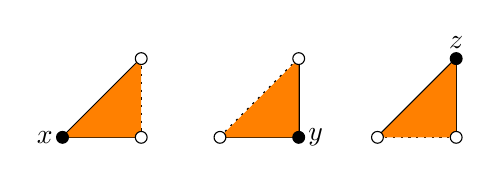
\begin{tikzpicture}
\node [left] at (0,0) {$x$};
\draw [dotted, thick] (1,1) -- (1,0);
\draw [thick] (0,0) -- (1,1);
\draw [thick] (0,0) -- (1,0);
\path [fill=orange] (0,0) -- (1,0) -- (1,1);
\draw [fill=white] ( 1,0) circle (0.075);
\draw [fill=white] ( 1,1) circle (0.075);
\draw [fill=black] ( 0,0) circle (0.075);

\node [right] at (3,0) {$y$};
\draw [thick] (3,1) -- (3,0);
\draw [dotted, thick] (2,0) -- (3,1);
\draw [thick] (2,0) -- (3,0);
\path [fill=orange] (2,0) -- (3,0) -- (3,1);
\draw [fill=black] ( 3,0) circle (0.075);
\draw [fill=white] ( 3,1) circle (0.075);
\draw [fill=white] ( 2,0) circle (0.075);

\node [above] at (5,1) {$z$};
\draw [thick] (5,1) -- (5,0);
\draw [thick] (4,0) -- (5,1);
\draw [dotted, thick] (4,0) -- (5,0);
\path [fill=orange] (4,0) -- (5,0) -- (5,1);
\draw [fill=white] ( 5,0) circle (0.075);
\draw [fill=black] ( 5,1) circle (0.075);
\draw [fill=white] ( 4,0) circle (0.075);
\end{tikzpicture}
\end{center}
The stars $x^*$ and $y^*$ share the open interior of the $1$-simplex $f$, so they glue on that piece. Moreover, they share the open interior of the $2$-simplex $(f,g)$, so the ``interiors'' are glued together too. What we are left with is the whole space minus the point $z$. So, $\ST(y) \cong X_\mathbf{C} - \{z\}$. Notice that $\ST(y) = \mu^{-1}_{\mathbf{C}}(U_y)$. For $\ST(z)$, we get the whole space $X_\mathbf{C}$. Again, $\ST(z) = \mu^{-1}_{\mathbf{C}}(U_z)$.
\end{example}

\begin{example}[The Finite Circle]
\label{ex:ST of our favorite finite space}
Take $\mathbf{C}$ to be the following poset: $a \leq c,d$, $b \leq c,d$. Then $\mathbf{C}$ may also be regarded as a finite $T_0$-space. The minimal opens are $U_a = \{a,c,d\}$, $U_b = \{b,c,d\}$, $U_c = \{c\}$ and $U_d = \{d\}$. The star sieve construction agrees with the inverse images of the McCord map.
\end{example}

\begin{example}[The Graph Category]
\label{ex:ST of the graph category}
Now it gets interesting. Take $\mathbf{C}$ to be the graph category $x \rightrightarrows y$, with $f,g : x \to y$. The realization $X_\mathbf{C}$ is a circle with two distinguished vertices $x$ and $y$. We have
\begin{align*}
\ST(x) &= x^*_{\id}, \\
\ST(y) &= x^*_f \sqcup x^*_g \sqcup y^*_{\id} / \sim.
\end{align*}
Let's compute
\begin{align*}
\st(x) &= \{x,f,g\}, \\
\st(y) &= \{y,f,g\}, \\
\st(f) &= \{f\}, \\
\st(g) &= \{g\}.
\end{align*}
Note that we leave out the degenerate simplices. 
The reader may convince himself that these are also taken care of during gluing. All possible morphisms in $\mathbf{C}/y$ are
\[ \begin{tikzcd}
x \arrow{r}{f} \arrow[swap]{dr}{f} & y \arrow{d}{\id} & x \arrow{r}{g} \arrow[swap]{dr}{g} & y \arrow{d}{\id} \\
& y & & y
\end{tikzcd}\]
Here, the open interior of the $1$-simplex $f$ is shared by the first copy $x^*_f$ and $y^*_{\id}$, so they glue on their top halves. The open interior of the $1$-simplex $g$ is shared by the second copy $x^*_g$ and $y^*_{\id}$, so they glue on their lower halves. What we are left with is a spiral that goes around $y$ once.
\[ \begin{tikzcd}
\ST(x) \arrow[equals]{d} & \; & \ST(y) \arrow[equals]{d} \\
\begin{tikzpicture}[tdplot_main_coords]
  
  \begin{scope}[color=black]
  \pgfplothandlerlineto
  \pgfplotfunction{\t}{-180,...,180}
       {\pgfpointxy {cos(\t)}{sin(\t)}{\t/360}} 
       \pgfusepath{stroke}
  \end{scope}

  \draw [fill=white] ( 1,0) circle (0.1);
  \draw [fill=black] (-1,0) circle (0.1);

  \node at (-1.4,0) {$x_{\id}$};

\end{tikzpicture} \arrow[shift left=1em, color=blue]{rr}{\ST(f)} \arrow[swap, shift right=1.5em, color=orange]{rr}{\ST(g)} \arrow[swap]{dr}{e_x} & \; & \begin{tikzpicture}[tdplot_main_coords]

  \begin{scope}[color=blue]
  \pgfplothandlerlineto
  \pgfplotfunction{\t}{-360,...,0}
       {\pgfpointxyz {cos(\t)}{sin(\t)}{-\t/360}} 
       \pgfusepath{stroke}
  \end{scope}

  \begin{scope}[color=orange, dashed]
  \pgfplothandlerlineto
  \pgfplotfunction{\t}{-180,...,0}
       {\pgfpointxyz {cos(\t)}{sin(\t)}{-\t/360}} 
       \pgfusepath{stroke}
  \end{scope}

  \begin{scope}[color=orange]
  \pgfplothandlerlineto
  \pgfplotfunction{\t}{0,...,130}
       {\pgfpointxyz {cos(\t)}{sin(\t)}{-\t/360}} 
       \pgfusepath{stroke}
  \end{scope}

  \begin{scope}[color=orange]
  \pgfplothandlerlineto
  \pgfplotfunction{\t}{145,...,360}
       {\pgfpointxyz {cos(\t)}{sin(\t)}{-\t/360}} 
       \pgfusepath{stroke}
  \end{scope}

  \begin{scope}[color=black, dashed]
  \pgfplothandlerlineto
  \pgfplotfunction{\t}{0,...,130}
       {\pgfpointxyz {cos(\t)}{sin(\t)}{-\t/360}} 
       \pgfusepath{stroke}
  \end{scope}

  \begin{scope}[color=black, dashed]
  \pgfplothandlerlineto
  \pgfplotfunction{\t}{145,...,180}
       {\pgfpointxyz {cos(\t)}{sin(\t)}{-\t/360}} 
       \pgfusepath{stroke}
  \end{scope}

  \draw [fill=black] ( 1,  0  ) circle (0.1);
  \draw [fill=black] (-1,  1  ) circle (0.1);
  \draw [fill=black] (-1, -1  ) circle (0.1);
  \draw [fill=white] ( 1, -1.8) circle (0.1);
  \draw [fill=white] ( 1,  1.8) circle (0.1);

  \node at (-1.3,1) {$x_f$};
  \node at (-1.3,-1) {$x_g$};
  \node at (1.4,0) {$y_{\id}$};

\end{tikzpicture} \arrow{dl}{e_y} \\
\; & \begin{tikzpicture}[tdplot_main_coords]
  
  \begin{scope}[color=black]
  \pgfplothandlerlineto
  \pgfplotfunction{\t}{-180,...,180}
       {\pgfpointxy {cos(\t)}{sin(\t)}{\t/360}} 
       \pgfusepath{stroke}
  \end{scope}

  \draw [fill=black] ( 1,0) circle (0.1);
  \draw [fill=black] (-1,0) circle (0.1);

  \node at (-1.3,0) {$x$};
  \node at ( 1.3,0) {$y$};

\end{tikzpicture}
& \; \\
\; & X_{\mathbf{C}} \arrow[equals]{u} & \;
\end{tikzcd} \]
\end{example}

\begin{example}[The Coequalizer Category]
\label{ex:ST of the coequalizer category}
Take $\mathbf{C}$ to be the coequalizer category $x \rightrightarrows y \to z$. Denote the morphisms by $f,g : x \to y$, $h : y \to z$, $hf = hg = k$. The realization $X_\mathbf{C}$ looks like a pancake, with vertex $x$ on the left border, vertex $z$ in the middle and $y$ on the right border. We have
\begin{align*}
\ST(x) &= x^*_{\id}, \\
\ST(y) &= x^*_f \sqcup x^*_g \sqcup y^*_{\id} / \sim, \\
\ST(z) &= x^*_k \sqcup y^*_h \sqcup z^*_{\id} / \sim.
\end{align*}
Let's compute
\begin{align*}
\st(x) &= \{x,f,g,k,(h,f),(h,g)\}, \\
\st(y) &= \{y,f,g,h,(h,f),(h,g)\}, \\
\st(z) &= \{z,h,k,(h,f),(h,g)\}, \\
\st(x) \cap \st(y) &= \{f,g,(h,f),(h,g)\}, \\
\st(x) \cap \st(z) &= \{k,(h,f),(h,g)\}, \\
\st(y) \cap \st(z) &= \{h,(h,f),(h,g)\}.
\end{align*}
Note that we leave out the degenerate simplices. 
The reader may convince himself that these are also taken care of during gluing.
The open set $x^*$ is the whole space $X_\mathbf{C}$ minus the closed line segment from $y$ to $z$. That is minus the closed $1$-simplex $h$. The open set $y^*$ is the whole space minus the closed line segment from $x$ to $y$. That is minus the closed $1$-simplex $k$. The open set $z^*$ is the interior of $X_\mathbf{C}$.
All possible morphisms in $\mathbf{C}/z$ are
\[ \begin{tikzcd}
z \arrow{r}{\id} \arrow[swap]{dr}{\id} & z \arrow{d}{\id} & y \arrow{r}{h} \arrow[swap]{dr}{h} & z \arrow{d}{\id} & x \arrow{r}{f} \arrow[swap]{dr}{k} & y \arrow{d}{h} & x \arrow{r}{g} \arrow[swap]{dr}{k} & y \arrow{d}{h} \\
& z & & z & & z & & z
\end{tikzcd} \]

\begin{itemize}
	\item[$\ST(x)$] The McCord space $\ST(x)$ is the open set $x^*$, the ``pacman face''.
	\item[$\ST(y)$] The interior of the $1$-simplex $f$ is shared by the first copy $x^*_f$ and $y^*_{\id}$, so they glue there. The interior of the $2$-simplex $(f,h)$ is shared by the first copy $x^*_f$ and $y^*_{\id}$, so they glue there. The interior of the $1$-simplex $g$ is shared by the second copy $x^*_g$ and $y^*_{\id}$, so they glue there. The interior of the $2$-simplex $(g,h)$ is shared by the second copy $x^*_g$ and $y^*_{\id}$, so they glue there. What we are left with is a spiral staircase making one roundabout.
	\item [$\ST(z)$] The $2$ copies of the $2$-simplex $(f,h)$ sitting inside $\ST(y)$ are shared by the same $2$-simplex $(f,h)$ sitting inside $z^*$, so they glue. The same holds for the $2$-simplex $(g,h)$. Moreover the simplices $k$ and $h$ glue too. So we are left with the whole space $X_\mathbf{C}$.
\end{itemize}
\end{example}

\begin{example}[The Equalizer Category]
\label{ex:ST of the equalizer category}
Take $\mathbf{C}$ to be the equalizer category $x \to y \rightrightarrows z$. Denote $h : x \to y$ and $f,g : y \to z$ with $fh = gh = k$. The realization $X_\mathbf{C}$ is again a pancake, but this time $y$ is at the left border, $x$ is in the middle and $z$ is at the right border. You can also view $X_\mathbf{C}$ as a coffee-filter, where the coffee runs down to the vertex $x$. We have
\begin{align*}
\ST(x) &= x^*, \\
\ST(y) &= x^* \sqcup y^* / \sim, \\
\ST(z) &= x^* \sqcup y^*_f \sqcup y^*_g \sqcup z^* / \sim.
\end{align*}
The open set $x^*$ is the whole space $X_\mathbf{C}$ minus the border, so minus the closed $1$-simplex $f$ and minus the closed $1$-simplex $g$. The open sets $y^*$ and $z^*$ are pacman faces.

\begin{itemize}
	\item [$\ST(x)$] This is the interior $x^*$ of $X_\mathbf{C}$.
	\item [$\ST(y)$] The interior of the $2$-simplex $(h,f)$ is shared by both $x^*$ and $y^*$, so they glue there. The interior of the $2$-simplex $(h,g)$ is shared by both $x^*$ and $y^*$, so they glue there. The interior of the $1$-simplex $h$ is shared by $x^*$ and $y^*$, so they glue there. What we are left with is the whole space $X_\mathbf{C}$ minus the point $z$.
	\item [$\ST(z)$] We go over the relevant morphisms in $\mathbf{C}/z$.
	\begin{itemize}
	\item [$k : x \to z$] We have $\st(x) \cap \st(z) = \{k, (h,f), (h,g)\}$. All three of those simplices have $k$ as a face. So $x^*$ and $z^*$ glue on the interiors of those three simplices.
	\item [$f : y \to z$] We have $\st(y) \cap \st(z) = \{f, g, (h,f), (h,g)\}$. The morphism $f$ is an eventual face of $f$ and $(h,f)$, so $y^*_f$ and $z^*$ glue on the interiors of $|f|$ and $|(h,f)|$.
	\item [$g : y \to z$] We have $\st(y) \cap \st(z) = \{f, g, (h,f), (h,g)\}$. The morphism $g$ is an eventual face of $g$ and $(h,g)$. So $y^*_g$ and $z^*$ glue on the interiors of $|g|$ and $|(h,g)|$.
	\end{itemize}
	What $\ST(z)$ looks like is hard to describe. It is sort of an oreo cookie with two infinitely close boundaries which twist at one end.
\end{itemize}
\end{example}

\begin{example}[The $2$-Element Monoid Category]
\label{ST of the 2-element monoid category}
Let $M$ be the monoid $\{1,f\}$ with $f^2 = f$, regarded as a category. The set of $n$-simplices of the nerve $NM$ are $(NM)_n = M^n$. In particular, $NM$ has just one vertex, call it $\bullet$. The realization $X_M$ is something which I cannot describe easily. It may be vaguely described as a ``fat'' point. We see that
\[ \st(\bullet) = \bigsqcup_{n \geq 0} \left(NM\right)_n. \]
In the slice category $M / \bullet$, all possible morphisms are
\[ \begin{tikzcd}
\bullet \arrow[swap]{dr}{1} \arrow{r}{1} & \bullet \arrow{d}{1} & \bullet \arrow[swap]{dr}{f} \arrow{r}{f} & \bullet \arrow{d}{1} & \bullet \arrow[swap]{dr}{f} \arrow{r}{f} & \bullet \arrow{d}{f} \\
& \bullet & & \bullet & & \bullet
\end{tikzcd} \]
Now the construction of $\mu(\bullet)$ goes as follows. We have the object $\bullet \xrightarrow{1} \bullet$ in $M/\bullet$ and the object $\bullet \xrightarrow{f} \bullet$ in $M/\bullet$. The realization $\bullet_1^*$ is $X_M$. The realization $\bullet_f^*$ is also $X_M$. What parts do we glue? The only valid morphism of the possible three above is $f : \bullet_f \to \bullet_1$. In other words, every simplex $\sigma \in \st(\bullet)$ which contains $f$ is glued between the two copies of $X_M$. What remains are the ``completely degenerate'' simplices $\sigma = (1,1,\ldots,1)$. But their realizations are just a point, so $\mu(\bullet)$ is $X_M$ with a ``double vertex'', akin to the well-known real line with double origin (which is indeed etale over the real line).
\end{example}

% \begin{proposition}
% \label{prop:ST is a faithful functor}
% $\ST : \mathbf{C} \to \mathbf{LH}/X_\mathbf{C}$ is a faithful functor.
% \end{proposition}
% \begin{proof}
% \begin{color}{red} Omitted for now. Remove this? It's not used anywhere. \end{color}
% \end{proof}
% \begin{proof}
% Suppose $A$ and $B$ are two objects of $\mathbf{C}$ and take $f,g \in \Hom_\mathbf{C}(A,B)$. Suppose that $\ST(f) = \ST(g)$. This means that for all $[h,p] \in \ST(A)$, we have $[f \circ h, p] = [g \circ h, p]$ in $\ST(B)$. Take $h = \id_A$. Then $[f,p] = [g,p]$ in $\ST(B)$ for all $p \in A^*$. Without loss of generality assume that $(f,p) \rhd (g,p)$. This means that there exists a morphism $k : f \to g$ in $\mathbf{C}/B$ and an $n$-simplex $\sigma \in \st(k)$ such that $p \in \Int(\sigma)$. Now $f$ and $g$ have the same domain and codomain, so $k$ is an endomorphism of $A$. Therefore $\st(k) = \st(A)$.
% % So there exists an $n$-simplex $\sigma \in \st(D)$ such that $f$ and $g$ are eventual faces of $\sigma$. Since $f$ and $g$ have the same codomain, this must mean that they are the same $1$-simplex, so $f=g$.
% \end{proof}

\section{Flatness Conditions}

To understand $\ST$ better, we shall study its fibers (or stalks).

\begin{definition}
\label{def:support at a point}
Let $p \in X_\mathbf{C}$. We define the \emph{support} of $p$ to be the full subcategory of $\mathbf{C}$ given by
\[ \mathbf{C}(p) := \left(\begin{array}{c} A \in \mathbf{C} : p \in A^* \\ + \\ \text{morphisms from $\mathbf{C}$} \end{array} \right). \]
\end{definition}
Note that $\mathbf{C}(p)$ is not the empty category by \cref{lem:realizations of stars form an open cover}. Put a relation on $\mathbf{C}(p)$ by declaring
\[ A \leq B \iff \Hom_\mathbf{C}(A,B) \neq \emptyset, \qquad A,B \in \mathbf{C}(p). \]
Then $\leq$ is a preorder, but usually not a partial order.

\begin{lemma}
\label{lem:different characterization of the support}
Let $p \in X_{\mathbf{C}}$. Then $p \in |\sigma|$ for a unique non-degenerate $n$-simplex $\sigma \in (N\mathbf{C})_n$. The objects of the category $\mathbf{C}(p)$ consist of the vertices of this $\sigma$.
\end{lemma}
\begin{proof}
If $A \in \mathbf{C}$ is a vertex of $\sigma$, then $\sigma \in \st(A)$. So $p \in A^*$. On the other hand, suppose that $A \in \mathbf{C}(p)$. We want to show that $A$ is a vertex of $\sigma$. We know that $p \in A^*$. So $p \in \Int(\tau)$ for some $\tau \in \st(A)$ by \cref{lem:realization of the star is union of the interiors}. So $p \in |\tau|$. Let $\sigma'$ be the unique non-degenerate simplex for $\tau$. Then $|\tau| = |\sigma'|$. Then $A$ is a vertex of $\sigma'$. By uniqueness, $\sigma = \sigma'$.
\end{proof}

Observe that if $p =|A|$ for some object $A \in \mathbf{C}$, then $\mathbf{C}(p)$ consists of a single object.

\begin{lemma}
If $\mathbf{C}$ is a finite poset, then $\mathbf{C}(p)$ is totally ordered with a minimal element for all $p \in X_{\mathbf{C}}$.
\end{lemma}
\begin{proof}
Take $p \in X_{\mathbf{C}}$. Let $\sigma$ be the unique non-degenerate simplex such that $p \in |\sigma|$. By \cref{lem:different characterization of the support}, the objects of the category $\mathbf{C}(p)$ are the vertices of $\sigma$. The vertices of an $n$-simplex in $(N\mathbf{C})_n$ are totally ordered, because $\mathbf{C}$ is a poset. Since $n < \infty$, there is a minimal element.
\end{proof}

The results of \cref{ex:ST of the three category} and \cref{ex:ST of our favorite finite space} generalize to a theorem. Recall that for a finite $T_0$-space $\mathbf{C}$, the McCord map $\mu_\mathbf{C}$ is defined to be the continuous map
\[ \mu_\mathbf{C} : X_{\mathbf{C}} \to \mathbf{C}, \qquad p \mapsto \min \mathbf{C}(p). \]

\begin{theorem}
\label{thm:mccord functor generalizes the mccord map}
Let $\mathbf{C}$ be a finite $T_0$-space, or equivalently a finite poset. For each $x \in \mathbf{C}$, denote its minimal open set around $x$ by $U_x$. Then there is a natural homeomorphism
\[ \ST(x) \cong \mu_\mathbf{C}^{-1}(U_x). \]
\end{theorem}
\begin{proof}
I claim that the etale map $e_x : \ST(x) \to X_\mathbf{C}$ has a section on $\mu_\mathbf{C}^{-1}(U_x) \subset X_\mathbf{C}$. Take a point $p \in \mu_\mathbf{C}^{-1}(U_x)$. Write $M_p = \min \mathbf{C}(p)$. 
Then $M_p \in U_x$, so $M_p \leq x$. Write $u : M_p \to x$ for the unique morphism. We now have $[u,p] \in \ST(x)$. 
Define
\[ s_x : \mu_\mathbf{C}^{-1}(U_x) \to \ST(x) \]
by sending the point $p$ to $[u,p]$. The definition of $s_x$ is unambiguous, because there is only one choice for $u$. Clearly we have $e_x \circ s_x = \id_{\mu_{\mathbf{C}}^{-1}\left(U_x \right)}$. So $s_x$ is a section. We shall now prove that $s_x \circ e_x = \id_{\ST(x)}$. Take $[g,p] \in \ST(x)$ and suppose that $(s_x \circ e_x)([g,p]) = [u,p]$. We want to show that $[g,p] = [u,p]$. Note that $g : D_g \to x$ is unique. Moreover, $D_g \in \mathbf{C}(p)$, so $M_p \leq D_g$. Let $h : M_p \to D_g$ be the unique morphism. Again by uniqueness, $h \circ g = u$. We now have a morphism $h : g \to u$ in $\mathbf{C}/x$, and $(g,h) \in \st(h)$ with $p \in \Int(g,h)$. So $[g,p] = [u,g]$.
\end{proof}

Thus, we have found a generalization of the McCord map.

% \begin{lemma}
% \label{lem:support at a vertex is a one-object category}
% If $p = |A| \in X_{\mathbf{C}}$ for some $A \in \mathbf{C}$, then the only object of $\mathbf{C}(p)$ is $A$, and the only morphisms of $\mathbf{C}(p)$ are the endomorphisms of $A$.
% \end{lemma}
% \begin{proof}
% Let $B$ be an object in the support of $p$. Then $p \in B^*$, so $p \in \Int(\sigma)$ for some $\sigma \in \st(B)$. But $p = |A|$, so the only possibility is that $\sigma$ is the $0$-simplex $B$, so $B=A$.
% \end{proof}

\begin{definition}
\label{def:alexandroff cat}
We say $\mathbf{C}$ is an \emph{Alexandroff} category if for all $p \in X_{\mathbf{C}}$
\begin{enumerate}
	\item the support $\mathbf{C}(p)$ is totally ordered with a (unique) minimal element $M_p$, and
	\item for every $A \in \mathbf{C}$ and for every $[f,p] \in e_A^{-1}(p)$ there exists a unique morphism $m : M_p \to D_f$ with the property that there is an $n$-simplex $\sigma \in \st(m)$ with $p \in \Int(\sigma)$.
	 % pair $(m, \sigma)$ with $m : M_p \to D_f$ a morphism in $\mathbf{C}$ and $\sigma \in \st(M_p) \cap (D_f)$ an $n$-simplex such that $m$ is eventually a face of $\sigma$.
\end{enumerate}
\end{definition}

\begin{remark}
I chose the name ``Alexandroff category'' because a topological space is termed an ``Alexandroff space'' when every point has a minimal open neighborhood with respect to inclusion. The second property is a technical one but it is required for \cref{lem:alexandroff implies well-fibered}.
\end{remark}

% \begin{remark}
% In \cref{def:alexandroff cat}, saying that the support of a point is totally ordered with a minimal element is the same thing as saying that there are no directed cycles in the underlying graph of the category.
% \end{remark}

\begin{example}
If $\mathbf{C}$ is a finite poset, then $\mathbf{C}$ is Alexandroff. The graph category from \cref{ex:ST of the graph category} is Alexandroff. The (co)equalizer category of \cref{ex:ST of the coequalizer category} and \cref{ex:ST of the equalizer category} is Alexandroff. The category $x \leftrightarrows y$ where the two arrows are each other's inverse, is not an Alexandroff category. On the other hand, its skeleton is the trivial category, so is Alexandroff. Hence being Alexandroff is an ``evil'' notion.
\end{example}

\begin{lemma}
\label{lem:alexandroff implies trivial endomorphisms}
If $\mathbf{C}$ is Alexandroff, then for all objects $A \in \mathbf{C}$ we have $\Hom_{\mathbf{C}}(A,A) = \{\id_A\}$.
\end{lemma}
\begin{proof}
Take $A \in \mathbf{C}$ and set $p = |A| \in X_{\mathbf{C}}$. Take an element $[f,p] \in e_A^{-1}(p)$ in the fiber. Then $f : D_f \to A$ and $p \in D_f^*$. By \cref{lem:different characterization of the support}, $D_f = M_p = A$. Then since $\mathbf{C}$ is Alexandroff, $f$ is unique, so we must have $f = \id_A$.
\end{proof}
From \cref{lem:alexandroff implies trivial endomorphisms} we see that being Alexandroff and a monoid at the same time implies that $\mathbf{C}$ is the trivial category with one object and one morphism. It also shows that being Alexandroff greatly restricts the category.

\begin{definition}
\label{def:well-fibered}
We say that $\mathbf{C}$ is \emph{well-fibered} if for all $p \in X_\mathbf{C}$ there exists an object $B \in \mathbf{C}$ such that $p^* \circ \ST \cong \Hom_\mathbf{C}(B,-)$.
\end{definition}

\begin{lemma}
\label{lem:alexandroff implies well-fibered}
If $\mathbf{C}$ is Alexandroff, then it is well-fibered.
\end{lemma}
\begin{proof}
Let $p \in X_{\mathbf{C}}$. The claim is that $p^* \circ \ST \cong \Hom_{\mathbf{C}}(M_p,-)$, where $M_p$ is defined as in \cref{def:alexandroff cat}. In other words, we need to find a natural isomorphism $\alpha : p^* \circ \ST \to \Hom_{\mathbf{C}}\left(M_p,-\right)$. To that end, define $\beta : \Hom_{\mathbf{C}}\left( M_p, - \right) \to p^* \circ \ST$ as follows. For each component $A \in \mathbf{C}$, we set 
\[ \beta_A : \Hom_{\mathbf{C}}\left(M_p,A \right) \to e^{-1}_A\left(p \right), \qquad h \mapsto [h,p]. \]
Then naturality of $\beta$ is clear. The natural transformation $\beta$ will be the inverse for the natural transformation $\alpha$. For the natural transformation $\alpha$, define it as follows.

% such that for every morphism $f : A \to B$ in $\mathbf{C}$ we have a commutative diagram
% \[ \begin{tikzcd}
% \left[ g,p \right] \arrow[mapsto]{d} & e_A^{-1}(p) \arrow{r}{\alpha_A} \arrow{d} & \Hom_\mathbf{C}(M_p, A) \arrow{d} & h \arrow[mapsto]{d} \\
% \left[ f \circ g, p \right]  & e_B^{-1}(p) \arrow{r}{\alpha_B} & \Hom_\mathbf{C}(M_p, B) & f \circ h
% \end{tikzcd} \]
Take $[g,p] \in e^{-1}_A(p)$. 
Then $g : D_g \to A$ and $p \in D_g^*$. 
So $D_g \in \mathbf{C}(p)$. Since $\mathbf{C}$ is Alexandroff, there exists a unique morphism $m : M_p \to D_g$ with the property that there is some $\sigma \in \st(m)$ such that $p \in \Int(\sigma)$. For each component $A \in \mathbf{C}$, we set
\[ \alpha_A : e^{-1}_A(p) \to \Hom_{\mathbf{C}}\left(M_p, A \right), \qquad [g,p] \mapsto g \circ m. \]
Because this $m$ is unique, $\alpha_A$ is well-defined. Observe now that
\[ \left(\beta_A \circ \alpha_A\right)[g,p] = [g \circ m, p]. \]
But $m$ has the property that we are also given a simplex $\sigma \in \st(m)$ such that $p \in \Int(\sigma)$. That means that $(g \circ m,p) \rhd (g,p)$, so $[g \circ m,p] = [g,p]$. In the other direction we find
\[ \left(\alpha_A \circ \beta_A \right)(h) = h, \]
so we conclude that $\alpha$ and $\beta$ are each other's inverse transformations.
% So every element in the fiber $e_A^{-1}(p)$ may be represented, in a unique way, as $[h,p]$ with $h : M_p \to A$ and $p \in M_p^*$. Define $\alpha_A : e^{-1}(p) \to \Hom_{\mathbf{C}}(M_p,A)$ by $[h,p] \mapsto h$. If $h = h'$, then $[h,p] = [h',p]$, and if $h \in \Hom_{\mathbf{C}}(M_p,A)$, then $[h,p] \in e^{-1}_A(p)$. So $\alpha_A$ is a bijection. If $f : A \to B$ is a morphism in $\mathbf{C}$ and $[h,p] \in e_A^{-1}(p)$, then
% \[ \alpha_B \left( [f \circ h, p] \right) = f \circ h = f \circ \alpha_A \left( [h, p] \right), \]
% so $\alpha$ is a natural isomorphism.
\end{proof}

\begin{lemma}
\label{lem:has enough points}
The topos $\mathbf{LH}/X_\mathbf{C}$ has enough points.
\end{lemma}
\begin{proof}
$X_\mathbf{C}$ is a geometric realization of a simplicial set, so $X_\mathbf{C}$ is a CW-complex by \cite[Proposition I.2.3]{goersjardinne09}. In particular it is a compactly generated Hausdorff space, and Hausdorff spaces always have enough points.
\end{proof}

Recall from \cref{def:set valued flat functor} that $\ST$ is flat when by definition the induced functor $- \otimes_{\mathbf{C}} \ST$ is left exact.

\begin{lemma}
\label{lem:well-fibered implies flat}
If $\mathbf{C}$ is well-fibered, then $\mu : \mathbf{C} \to \mathbf{LH}/X_{\mathbf{C}}$ is flat.
\end{lemma}
\begin{proof}
By \cref{lem:has enough points}, it suffices to prove that for every $p \in X_{\mathbf{C}}$ the functor $p^* \circ \mu : \mathbf{C} \to \mathbf{Set}$ is flat. This is the same thing as proving that the category of elements $\int_{\mathbf{C}} \left( p^* \circ \mu \right)$ is filtered, by \cref{thm:flat iff filtering}. Since $\mathbf{C}$ is well-fibered, there exists some object $B \in \mathbf{C}$ such that $p^* \circ \mu \cong \Hom_{\mathbf{C}}\left(B,-\right)$. Therefore,
\[ \int_\mathbf{C} \left( p^* \circ \mu \right) \cong \int_{\mathbf{C}} \Hom_{\mathbf{C}}\left(B, - \right) \cong B \backslash \mathbf{C}. \]
Now the over-category $B \backslash \mathbf{C}$ is always filtered, because $\id_B : B \to B$ is an initial object.
\end{proof}

So we see that when $\mathbf{C}$ is Alexandroff, $\mu$ is flat.

\begin{lemma}
Assume that $\mathbf{C}$ is a monoid (so consists of a single object). Let $p \in X_{\mathbf{C}}$. Denote the unique object of $\mathbf{C}$ by $\bullet$. Let $e_\bullet : \mu(\bullet) \to X_\mathbf{C}$ be the etale space of $\bullet$.
\begin{enumerate}
	\item If $p = |\bullet|$, then $e_\bullet^{-1}(|\bullet|) \cong \Hom_\mathbf{C}(\bullet, \bullet)$.
	\item If $p \neq |\bullet|$, then $e_\bullet^{-1}(p)$ is a one-element set.
\end{enumerate}
\end{lemma}
\begin{proof}
Follows from the definition of $\ST(\bullet)$.
\end{proof}

We'll end this section with a conjecture.

\begin{conjecture}
\label{conj:if C is a monoid then ST is flat}
If $\mathbf{C}$ is a monoid, then $\mu : \mathbf{C} \to \mathbf{LH}/X_{\mathbf{C}}$ is flat.
\end{conjecture}

The evidence lies in the fact that $X_\mathbf{C}$ may be regarded as the classifying space of the monoid $\mathbf{C}$, so its fundamental group is the groupification of $\mathbf{C}$ (for instance, see \cite{lenz2011}). Moreover, the fundamental group of the presheaf topos on $\mathbf{C}$ is (the profinite completion of) the groupification of $\mathbf{C}$. So in this sense, the McCord functor $\ST$ should detect that.
	%!TEX root = main.tex
%
% isomorphism.tex
%

\chapter{The Equivalence}

In this section, we assume that $\mathbf{C}$ is an Alexandroff category (viz. \cref{def:alexandroff cat}). Recall (viz. \cref{def:star sieve}) that we constructed a flat (viz. \cref{lem:well-fibered implies flat}, \cref{lem:alexandroff implies well-fibered}) functor
\[ \ST : \mathbf{C} \to \mathbf{LH}/X_{\mathbf{C}}. \]
We shall make some preparations first by proving some useful propositions, and then finish by proving that we can restrict to an equivalence of categories on the level of locally constant finite objects.
\section{Preparation}

\begin{proposition}
\label{prop:the geometric morphism induced by ST}
There exists a geometric morphism
\[ \tau(\ST) : \mathbf{LH}/X_{\mathbf{C}} \to \mathbf{Set}^{\mathbf{C}^{op}} \]
for which the left-exact left adjoint $\tau(\ST)^*$ is given by sending a presheaf $P$ on $\mathbf{C}$ to the tensor product $P \otimes_{\mathbf{C}} \ST$, and for which the right adjoint $\tau(\ST)_*$ sends an etale space $e : E \to X_{\mathbf{C}}$ to the presheaf $\underline{\Hom}_{\mathbf{LH}/X_{\mathbf{C}}}\left(\ST, E\right)$ defined for every object $A \in \mathbf{C}$ by
\[ \underline{\Hom}_{\mathbf{LH}/X_{\mathbf{C}}}\left(\ST, E \right)(A) = \Hom_{\mathbf{LH}/X_{\mathbf{C}}}\left(\ST(A), E \right). \]
\end{proposition}
\begin{proof}
Follows directly from the theory in \cite[Chapter VII, Paragraph 7]{MacLaneMoerdijk91}. In particular, in \cite[Theorem VII.7.2]{MacLaneMoerdijk91}, take $\mathscr{E} = \mathbf{LH}/X_{\mathbf{C}}$. Alternatively, we spoke of the bijection between flat functors and geometric morphisms in \cref{thm:geometric morphisms correpsond to flat functors to E}.
\end{proof}
% Let $\mathbf{C} \in \mathbf{Cat}$ be a small category. Assume that $X_{\mathbf{C}}$ is connected. If $\mu : \mathbf{C} \to \mathbf{LH}/X_{\mathbf{C}}$ denotes the etale functor, recall that we get a sheaf by applying the sheaf of sections functor $\Gamma : \mathbf{LH}/X_{\mathbf{C}} \to \Sh(X_{\mathbf{C}})$.
% Explicitly, this means that $(\Gamma \mu)(A)$ is the sheaf defined by sending an open $U \subset X_{\mathbf{C}}$ to the set of sections
% \[ (\Gamma \mu)(A)(U) = \{s : U \to \ST(A) \mid e_A \circ s = \id_U \} \]
% From \ref{lem:well-fibered implies flat} we obtain the following.
% \begin{corollary}
% Let $\mathbf{C} \in \mathbf{Cat}$ be an Alexandroff category. Then there is a flat functor $\mathbf{C} \to \Sh(X_\mathbf{C})$ given by sending an object $A \in \mathbf{C}$ to the sheaf $(\Gamma \mu)(A)$.
% \end{corollary}
% \begin{proof}
% \cite[Theorem II.3]{MacLaneMoerdijk91} gives an equivalence of categories $\Sh(X_\mathbf{C}) \cong \mathbf{LH}/X_{\mathbf{C}}$ via $ \Gamma \dashv \Lambda$.
% \end{proof}

 

% \begin{proposition}
% \label{prop:the geometric morphism induced by ST}
% Let $\mathbf{C} \in \mathbf{Cat}$ be an Alexandroff category. Then there exists a geometric morphism $\tau(\Gamma \ST) : \mathbf{LH}/X_{\mathbf{C}} \to \mathbf{Set}^{\mathbf{C}^{op}}$ for which the left-exact left adjoint is given by
% \[ \tau(\Gamma \ST)^* = -\otimes_{\mathbf{C}} \Gamma \ST \]
% and the right adjoint is given by
% \[ \tau(\Gamma \ST)_* = \underline{\Hom}_{\Sh(X_{\mathbf{C}})} \left(\Gamma \ST, - \right). \]
% \end{proposition}
% \begin{proof}
% Follows directly from \cite[Chapter VII, Paragraph 7]{MacLaneMoerdijk91}. Indeed, $\tau(\Gamma \mu)^*$ is left-exact because $\mu$ (and so also $\Gamma \mu$) is flat by \cref{lem:well-fibered implies flat} and \cref{lem:alexandroff implies well-fibered}. They are adjoint by the generalized ``$\Hom\text{-}\otimes$'' adjunction, see \cite[Theorem VII.2.1]{MacLaneMoerdijk91}.
% \end{proof}

% From this point on, we assume that $\mathbf{C}$ is an Alexandroff category. 

We shall be needing the following proposition.

\begin{proposition}
\label{prop:if two maps agree on a point then they are equal from szamuely}
Let $p : Y \to X$ be a (not necessarily finite) covering map, where $Y$ is a topological space and $X$ is a locally connected space. Let $f,g : Z \to Y$ be two continuous maps satisfying $p \circ f= p \circ g$, where $Z$ is a connected topological space. If there is a point $z \in Z$ with $f(z) = g(z)$, then $f=g$.
\end{proposition}
\begin{proof}
This is \cite[Proposition 2.2.2]{szamuely}. We'll give a sketch of the proof here. Let $U = \{w \in Z : f(w) = g(w)\}$. Then prove that $U$ is both open and closed in $Z$. Conclude that $U$ must be all of $Z$ by connectedness.
\end{proof}

The following proposition is central to this section.

\begin{proposition}
\label{coro:number of LHs is d if the degree is d}
Let $\pi_E : E \to X_\mathbf{C}$ be a finite covering map of degree $d>0$ and let $A$ be an object of $\mathbf{C}$. Then we have a natural bijection of sets
\[ \alpha_{A,E} : \left(\mathbf{LH}/X_\mathbf{C} \right)\left(\mu A, E \right) \to \pi_E^{-1}(|A|), \qquad \varphi \mapsto \varphi[\id_A, |A|]. \]
\end{proposition}
\begin{proof}
By \cref{lem:alexandroff implies trivial endomorphisms},
\[ e_A^{-1}(|A|) = \left\{ \left[ \id_A, |A| \right] \right\} \subset \ST(A). \]
Write
\[ \pi_E^{-1}(|A|) = \{x_1,\ldots,x_d\} \subset E. \]
Now take a morphism $\varphi \in (\mathbf{LH}/X_{\mathbf{C}})(\ST(A), E)$. Then
\[ \varphi[\id_A, |A|] \in \{x_1,\ldots,x_d\}. \]
I claim that these $d$ choices for $\varphi[\id_A,|A|]$ completely determine $\varphi$. 
So let $\psi \in (\mathbf{LH}/X_{\mathbf{C}})(\ST(A),E)$ be another morphism and suppose that
\[ \varphi[\id_A,|A|] = x_1 = \psi[\id_A,|A|]. \]
We will apply \cref{prop:if two maps agree on a point then they are equal from szamuely}. 
Take $Y = E$, $X = X_{\mathbf{C}}$, $Z = \ST(A)$, $p = \pi_E$, $f = \varphi$, $g = \psi$ and $z = [\id_A,|A|]$ in \cref{prop:if two maps agree on a point then they are equal from szamuely}. 
Then $X_{\mathbf{C}}$ is a locally connected space, because it is a CW-complex by \cite[Proposition I.2.3]{goersjardinne09}. Moreover, $\ST(A)$ is connected by \cref{lem:ST is connected for every object A}. Finally,
\[ p \circ f = \pi_E \circ \varphi = e_A = \pi_E \circ \varphi = p \circ g. \]
This proves that
\[ \# \left(\mathbf{LH}/X_\mathbf{C} \right)\left(\mu A, E \right) \leq d. \]
Let us now prove that the map $\alpha_{A,E}$ is surjective. 
Thus, given $x \in \pi_E^{-1}(|A|)$ we want to show that there exists some $\varphi \in (\mathbf{LH}/X_{\mathbf{C}})(\ST A, E)$ such that $\varphi[\id_A,|A|] = x$. We shall actually construct such a $\varphi$. First, observe that $\pi_E$ is a Serre fibration. Then apply \cref{prop:if two maps agree on a point then they are equal from szamuely} to see that any two lifts of some $|\sigma| : \Delta^n \to X_{\mathbf{C}}$ are unique. For each $f \in \mathbf{C}/A$ (and so in particular for $\id_A$) we have a commutative diagram
\[ \begin{tikzcd}
\Delta^0 \arrow[hook]{r}{x} \arrow[hook, swap]{d}{|d_0|} & E \arrow{d}{\pi_E} \\
\Delta^1 \arrow[swap]{r}{|f|} \arrow[dashed]{ur}{\exists ! \widetilde{f}} & X_{\mathbf{C}} \end{tikzcd} \]
and a unique diagonal filler $\widetilde{f} : \Delta^1 \to E$ as indicated by the dotted arrow in the diagram. Thus we have a collection of lifted paths $\widetilde{f} : \Delta^n \to E$ all ending up at the point $x \in E$ and starting at some arbitrary point in $E$. Let us call the starting point $\widetilde{f}(0)$. 

% Then for each pair $f,g \in \mathbf{C}/A$ and for each morphism $h : f \to g$ in $\mathbf{C}/A$ we have two commutative diagrams
% \[ \begin{tikzcd}
% \Delta^0 \arrow[hook, swap]{d}{|d^0|} \arrow[hook]{r}{\widetilde{g}(0)} & E \arrow{d}{\pi_E} & \Delta^0 \arrow[hook, swap]{d}{|d^1|} \arrow[hook]{r}{\widetilde{f}(0)} & E \arrow{d}{\pi_E} \\
% \Delta^1 \arrow[swap]{r}{|h|} \arrow[dotted]{ur}{\exists ! \widetilde{h}_1} & X_{\mathbf{C}} & \Delta^1 \arrow[swap]{r}{|h|} \arrow[dotted]{ur}{\exists ! \widetilde{h}_2} & X_{\mathbf{C}}
% \end{tikzcd} \]
% and diagonal fillers $\widetilde{h}_1, \widetilde{h}_2 : \Delta^1 \to E$. By continuity and commutativity of the diagrams, $\widetilde{h}_1(0) = \widetilde{h}_2(0)$, $\widetilde{h}_1(1) = \widetilde{h}_2(1)$, so that $\widetilde{h}_1 = \widetilde{h}_2$ by uniqueness.

Now let $[f,p] \in \ST(A)$ be an arbitrary point. We are going to define what $\varphi[f,p]$ is. We have $f : D_f \to A$ and $p \in D_f^*$, so $p \in \Int(\sigma)$ for some $n$-simplex $\sigma \in \st(D_f)$. We may assume that $\sigma$ is non-degenerate by \cref{lem:eilenberg-zilber}.
If $n=0$, then $p=|D_f|$. In that case, we define
\[ \varphi[f,p] := \widetilde{f}(0). \]
Suppose now that $n>0$. Let $\theta : \mathbf{0} \to \mathbf{n}$ be an injective order-preserving map as in \cref{eq:sigma is eventual face of tau diagram} such that $D_f = \sigma \circ \mathbf{\Delta}(-,\theta)$. Then we have a commutative diagram
\[ \begin{tikzcd}
\Delta^0 \arrow[hook]{r}{\widetilde{f}(0)} \arrow[hook, swap]{d}{|\mathbf{\Delta}(-,\theta)|} & E \arrow{d}{\pi_E} \\
\Delta^n \arrow[swap]{r}{|\sigma|} \arrow[dashed]{ur}{\exists ! \widetilde{\sigma}} & X_{\mathbf{C}} \end{tikzcd} \]
and a unique diagonal filler $\widetilde{\sigma} : \Delta^n \to E$.  
Let $t \in \Delta^n$ be the unique coordinates such that $p = |\sigma|(t)$. We define
\[ \varphi[f,p] := \widetilde{\sigma}(t). \]
We must prove that this definition is independent of the chosen representative of the equivalence relation in $\ST(A)$. 
So suppose that $(f,p) \rhd (g,p)$. Then $p \in \Int(\sigma_f)$ and $p \in \Int(\sigma_g)$ for some $\sigma_f$ having $D_f$ as a vertex and some $\sigma_g$ having $D_g$ as a vertex. Suppose that we have uniquely lifted $\sigma_f$ and $\sigma_g$ to maps
\[ \Delta^n \xrightarrow{\widetilde{\sigma_f}} E, \qquad \Delta^m \xrightarrow{\widetilde{\sigma_g}} E. \]
Let $t_f \in \Delta^n$ and $t_g \in \Delta^m$ be the unique coordinates such that
\[ |\sigma_f|(t_f) = p = |\sigma_g|(t_g). \]
By the definition of $\rhd$, There exists a morphism $h : f \to g$ in $\mathbf{C}/A$ and a $k$-simplex $\tau \in \st(h)$ such that $p \in \Int(\tau)$. Consider first the $2$-simplex $\beta$ given by
\[ \beta = (h,g) : \mathbf{\Delta}(-, \mathbf{2}) \to N\mathbf{C}. \]
Let $\widetilde{\beta} : \Delta^2 \to E$ be the unique lift of $|\beta| : \Delta^2 \to X_{\mathbf{C}}$. By \cite[Exercise A.1]{AlgebraicTopologyBible}, the face of a lift is the lift of a face, so we see that two of the faces of $\widetilde{\beta}$ upstairs in $E$ are the lifts $\widetilde{f}$ and $\widetilde{g}$. Denote by $\widetilde{h}$ the third lift of $|h| : \Delta^1 \to X_{\mathbf{C}}$.

We may assume by \cref{lem:eilenberg-zilber} that $\tau$, $\sigma_f$ and $\sigma_g$ are non-degenerate.
This implies that $\tau = \sigma_f = \sigma_g$, and $n=m=k$, and $t_f = t_g$. Let $\theta' : \mathbf{1} \to \mathbf{m}$ be an injective order-preserving map as in \cref{eq:sigma is eventual face of tau diagram} such that $h = \tau \circ \mathbf{\Delta}(-,\theta')$. Then we have a commutative diagram
\[ \begin{tikzcd}
\Delta^1 \arrow{r}{\widetilde{h}} \arrow[hook, swap]{d}{|\mathbf{\Delta}(-,\theta')|} & E \arrow{d}{\pi_E} \\
\Delta^m \arrow[swap]{r}{|\tau|} \arrow[dashed]{ur}{\exists ! \widetilde{\tau}} & X_{\mathbf{C}} \end{tikzcd} \]
By uniqueness of the lifts, $\widetilde{\sigma_f} = \widetilde{\sigma_g} = \widetilde{\tau}$.
% and suppose that for each of the $n+1$ faces $d_0 \sigma, \ldots, d_n \sigma$ of $\sigma$ a lift
% \[ \widetilde{d_i \sigma} : \Delta^{n-1} \to E \]
% has been chosen (if $\sigma$ is a $2$-simplex, the $3$ lifts are unique). We have $n+1$ commutative diagrams
% \[ \begin{tikzcd}
% \Delta^{n-1} \arrow[hook, swap]{d}{|d^i|} \arrow{r}{\widetilde{d_i \sigma}} & E \arrow{d}{\pi_E} \\
% \Delta^n \arrow[swap]{r}{|\sigma|} \arrow[dotted]{ur}{\exists \widetilde{\sigma}_i} & X_{\mathbf{C}}
% \end{tikzcd} \qquad i=0,\ldots,n. \]
% Since $\pi_E : E \to X_{\mathbf{C}}$ is a Serre fibration, there exist $n+1$ diagonal fillers $\widetilde{\sigma}_i : \Delta^n \to E$ making the two triangles commute in each of the $n+1$ corresponding diagrams. These diagonal fillers are still unique by connectedness of $\Delta^n$, and the fact that $\pi_E$ is a covering map, so the image of a lift cannot cross between disjoint open sheets in $E$ upstairs.
% Now commutativity and continuity imply that each of the $n+1$ lifts $\widetilde{\sigma}_i$ for $|\sigma|$ are the same, so we will denote this single lift by $\widetilde{\sigma} : \Delta^n \to E$. Since $p \in \Int(\sigma)$, there are (unique) barycentric coordinates $(t_0,\ldots,t_n) \in \Delta^n$ with $t_i > 0$ for all $i$ such that
% \[ |\sigma|(t_0,\ldots,t_n) = p.\]
% We define
% \[ \varphi[f,p] := \widetilde{\sigma}\left(t_0,\ldots,t_n\right). \]
% By construction, $\varphi$ is a map with the property that $e_A = \pi_E \circ \varphi$, so what's left to do is to check that it is independent of the equivalence relation, and that it is continuous.

% So suppose that $(f,p) \rhd (g,p)$ (see \cref{def:star sieve}). Then there exists a morphism $h : f \to g$ in $\mathbf{C}/A$ and an $m$-simplex $\tau \in \st(h)$ such that $p \in \Int(\tau)$. We have $p \in D_f^*$, so there is some $\sigma_f \in \st(D_f)$ with $p \in \Int(\sigma_f)$ and we have $p \in D_g^*$, so there is some $\sigma_g \in \st(D_g)$ with $p \in \Int(\sigma_g)$. By \cref{lem:eilenberg-zilber} we may assume that $\sigma_f$, $\sigma_g$ and $\tau$ are non-degenerate. But then they must all three be the same simplex. So $\varphi$ is well-defined.

Continuity of $\varphi$ follows from the fact that all the liftings $\widetilde{\sigma} : \Delta^n \to E$ from the continuous maps $|\sigma| : \Delta^n \to X_{\mathbf{C}}$ are continuous. Moreover, the realization $X_{\mathbf{C}}$ is defined as the colimit
\[ X_{\mathbf{C}} = \colim_{\stackrel{\mathbf{\Delta}(-,\mathbf{n}) \to N\mathbf{C}}{\text{in } \mathbf{\Delta} \downarrow N\mathbf{C}}}\Delta^n \]
So the gluing data comes from $X_{\mathbf{C}}$.

\end{proof}

From \cref{def:tensor product} and \cref{eq:tensor product rule}, we see that $P \otimes_{\mathbf{C}} \ST$ can be described as the space
\[ \left( \bigsqcup_{A \in \mathbf{C}} P(A) \times \ST(A) \right) / \sim, \]
where elements of this space (wherein $P(A)$ carries the discrete topology for each $A \in \mathbf{C}$) are denoted by
\[ x \otimes [f,p] \in P \otimes_{\mathbf{C}} \ST, \qquad A \in \mathbf{C},\, x \in P(A), \, [f,p] \in \ST(A) \]
under the rule
\[ x \cdot g \otimes [f,p] = x \otimes [g \circ f, p], \qquad x \in P(A), g : A \to B, [f,p] \in \ST(A) \]
defined by the equivalence relation $\sim$. In particular, we note that if $P$ is representable, say $P = \Hom_{\mathbf{C}}(-,A)$ with $A \in \mathbf{C}$, then
\[ \Hom_{\mathbf{C}}(-,A) \otimes_{\mathbf{C}} \ST \cong \ST(A). \]

\begin{theorem}
\label{thm:equivalence of categories}
If $\pi : E \to X_{\mathbf{C}}$ is a finite covering map, then $\underline{\Hom}_{\mathbf{LH}/X_{\mathbf{C}}}\left(\ST, E \right)$ is a locally constant finite presheaf on $\mathbf{C}$. Conversely, if $P$ is a locally constant finite presheaf on $\mathbf{C}$, then $P \otimes_{\mathbf{C}} \ST$ has the structure of a finite covering space over $X_{\mathbf{C}}$.
\end{theorem}
\begin{proof}
The claim that $P \otimes_{\mathbf{C}} \ST$ is a finite covering map whenever $P \in \left(\mathbf{Set}^{\mathbf{C}^{op}}\right)_{\lcf}$ is covered in \cref{prop:standard LCF properties for the LCF topos}. (Use \cref{thm:equivalence of categories between etale spaces and sheaves} there for the translation between sheaves and etale spaces). Explicitly, the finite covering map is given by
\[ \pi : P \otimes_{\mathbf{C}} \ST \to X_{\mathbf{C}}, \qquad x \otimes [f,p] \mapsto p. \]
The degree of $\pi$ is the number of elements in $P(A)$, for any $A \in \mathbf{C}$. This is well-defined by \cref{prop:locally constant iff every restriction map is a bijection} and the assumption that $X_{\mathbf{C}}$ is connected.

We shall prove the other direction, which is the remarkable one. So we want to show that given a finite covering map $\pi_E : E \to X_\mathbf{C}$ and given a morphism $f : A \to B$ in $\mathbf{C}$, the map
\begin{equation}
\label{eq:ST hom map between locally const finites}
(\mathbf{LH}/X_\mathbf{C})(\ST B, E) \to (\mathbf{LH}/X_\mathbf{C})(\ST A, E), \qquad \varphi \mapsto \varphi \circ \ST(f)
\end{equation}
is a bijection. By \cref{coro:number of LHs is d if the degree is d}, it suffices to prove that the map in \cref{eq:ST hom map between locally const finites} is injective. So take two morphisms $\varphi, \psi \in (\mathbf{LH}/X_\mathbf{C})(\ST B, E)$ and suppose that $ \varphi \circ \ST(f) = \psi \circ \ST(f)$. We want to prove that $\varphi = \psi$. In \cref{prop:if two maps agree on a point then they are equal from szamuely}, take $Y = E$, $X = X_{\mathbf{C}}$, $Z = \ST(B)$, $p = \pi_E$, $f = \varphi$, $g = \psi$. As in the proof of \cref{coro:number of LHs is d if the degree is d}, all conditions of \cref{prop:if two maps agree on a point then they are equal from szamuely} are satisfied, except that we need to supply a point $[h,p] \in \ST(B)$ such that $\varphi[h,p] = \psi[h,p]$. But we know that
\[ \forall \; [g,p] \in \ST(A) : \varphi[f \circ g,p] = \psi[f \circ g, p]. \]
Now $\ST(A)$ is non-empty, because $[\id_A, |A|] \in \ST(A)$. Therefore
\[ \varphi[f, |A|] = \psi[f, |A|] \]
and we are done.
\end{proof}

% \begin{theorem}
% \label{thm:equivalence of categories}
% If $E \in \Sh(X_{\mathbf{C}})_{\lcf}$ is a locally constant finite sheaf, then $\underline{\Hom}_{\Sh(X_{\mathbf{C}})}\left(\Gamma \ST, E \right)$ is a locally constant finite presheaf. 
% Conversely, if $P \in \left(\mathbf{Set}^{\mathbf{C}^{op}}\right)_{\lcf}$ is a locally constant finite presheaf, then $P \otimes_{\mathbf{C}} \Gamma \ST$ is a locally constant finite sheaf.
% \end{theorem}
% \begin{proof}
% The claim that $P \otimes_{\mathbf{C}} \Gamma \ST$ is a locally constant finite sheaf whenever $P \in \left(\mathbf{Set}^{\mathbf{C}^{op}}\right)_{\lcf}$ is covered in \cite[Proposition 8.42]{johnstone77}. We shall prove the other direction, which is the remarkable one.

% Because $\Gamma$ is left adjoint to $\Lambda$, we have, for all objects $A \in \mathbf{C}$ and for all sheaves $F$ on $X_\mathbf{C}$, a bijection of sets
% \[ \Sh(X_\mathbf{C})\left( \Gamma \ST A, F \right) \cong (\mathbf{LH}/X_\mathbf{C})\left( \ST A, \Lambda F \right). \]
% If $F$ is a locally constant finite sheaf on $X_\mathbf{C}$, then $\Lambda F$ is a finite covering map on $X_\mathbf{C}$. Also, by \cref{prop:locally constant iff every restriction map is a bijection}, showing that $\Sh(X_\mathbf{C} )\left(\Gamma \ST(-), F \right)$ is a locally constant finite presheaf is equivalent to showing that all of its restriction maps are bijections. Putting these observations together, we want to show that given a finite covering map $\pi_E : E \to X_\mathbf{C}$ and given a morphism $f : A \to B$ in $\mathbf{C}$, the map
% \begin{equation}
% \label{eq:ST hom map between locally const finites}
% (\mathbf{LH}/X_\mathbf{C})(\ST B, E) \to (\mathbf{LH}/X_\mathbf{C})(\ST A, E), \qquad \varphi \mapsto \varphi \circ \ST(f)
% \end{equation}
% is a bijection. By \cref{coro:number of LHs is d if the degree is d}, it suffices to prove that the map in \cref{eq:ST hom map between locally const finites} is injective. So take two morphisms $\varphi, \psi \in (\mathbf{LH}/X_\mathbf{C})(\ST B, E)$ and suppose that $ \varphi \circ \ST(f) = \psi \circ \ST(f)$. We want to prove that $\varphi = \psi$. In \cref{prop:if two maps agree on a point then they are equal from szamuely}, take $Y = E$, $X = X_{\mathbf{C}}$, $Z = \ST(B)$, $p = \pi_E$, $f = \varphi$, $g = \psi$. As in the proof of \cref{coro:number of LHs is d if the degree is d}, all conditions of \cref{prop:if two maps agree on a point then they are equal from szamuely} are satisfied, except that we need to supply a point $[h,p] \in \ST(B)$ such that $\varphi[h,p] = \psi[h,p]$. But we know that
% \[ \forall \; [g,p] \in \ST(A) : \varphi[f \circ g,p] = \psi[f \circ g, p]. \]
% Now $\ST(A)$ is non-empty, because $[\id_A, |A|] \in \ST(A)$. Therefore
% \[ \varphi[f, |A|] = \psi[f, |A|] \]
% and we are done.
% \end{proof}

\begin{lemma}
\label{lem:fiber of the tensor product P otimes ST is PA}
Let $P$ be a locally constant finite presheaf on $\mathbf{C}$ and take an object $A \in \mathbf{C}$. Then the fiber of the finite covering map $\pi : P \otimes_\mathbf{C} \ST \to X_{\mathbf{C}}$ above $|A| \in X_{\mathbf{C}}$ is given by
\[ \pi^{-1} \left( |A| \right) = \left\{ x \otimes [\id_A,|A|] : x \in P(A) \right\} \]
and thus there is an isomorphism of presheaves $\pi^{-1}(|-|) \cong P$ on $\mathbf{C}$.
\end{lemma}
\begin{proof}
We have
\begin{align*}
\pi^{-1}(|A|) &= \left\{ x \otimes [f,p]               : x \in P(B),\, f : D_f \to B,\, p = |A| \in D_f^*,\, B \in \mathbf{C} \right\} \\
              &= \left\{ x \otimes [f,|A|]             : x \in P(B),\, f : A   \to B,\, B \in \mathbf{C} \right\} \\
              &= \left\{ x \cdot f \otimes [\id_A,|A|] : x \in P(B),\, f : A \to B,\, B \in \mathbf{C} \right\} \\
              &= \left\{ P(f)(x) \otimes [\id_A, |A|]  : x \in P(B),\, f \in \Hom(A,B),\, B \in \mathbf{C} \right\} \\
              &= \left\{ x \otimes [\id_A, |A|]        : x \in P(A) \right\}.
\end{align*}
In the second equality, we use the fact that $D_f^*$ has $|D_f|$ as its only ``vertex'', so that $D_f = A$. In the third equality we use the tensor product rule, and in the last equality we use the fact that $P(f)$ is a bijection for all $f$ by \cref{prop:locally constant iff every restriction map is a bijection} and \cref{lem:alexandroff implies trivial endomorphisms}.
\end{proof}

\begin{corollary}
\label{coro:number of LHs if size of P(A) from ST(A) to the tensor product}
Let $P$ be a locally constant finite presheaf on $\mathbf{C}$. For every $A \in \mathbf{C}$, we have a natural bijection of sets
\[ \left(\mathbf{LH}/X_{\mathbf{C}}\right)\left(\ST(A), P \otimes_{\mathbf{C}}\ST \right) \cong P(A). \]
\end{corollary}
\begin{proof}
Combine the results of \cref{coro:number of LHs is d if the degree is d}, \cref{thm:equivalence of categories} and \cref{lem:fiber of the tensor product P otimes ST is PA}.
\end{proof}

The category of finite covering spaces over $X_{\mathbf{C}}$ is denoted by $\mathbf{FinCov}/X_{\mathbf{C}}$. It is a full subcategory of $\mathbf{LH}/X_{\mathbf{C}}$. The equivalence of categories in \cref{thm:equivalence of categories between etale spaces and sheaves} restricts to an equivalence
\[ \mathbf{FinCov}/X_{\mathbf{C}} \cong \Sh(\mathcal{O}(X_{\mathbf{C}}))_{\lcf}. \]

\begin{corollary}
Let $\pi_E : E \to X_{\mathbf{C}}$ be a finite covering space. Consider the finite covering space $\pi : \underline{\Hom}(\ST,E) \otimes \ST \to X_{\mathbf{C}}$. Then for each object $A \in \mathbf{C}$, we have a natural bijection of fibers (i.e. stalks)
\[ \pi^{-1}(|A|) \cong \pi_E^{-1}(|A|). \]
\end{corollary}
\begin{proof}
By \cref{lem:fiber of the tensor product P otimes ST is PA}, we have
\[ \pi^{-1}(|A|) \cong \Hom\left(\ST(A), E \right). \]
And by \cref{coro:number of LHs is d if the degree is d},
\[ \Hom\left(\ST(A), E \right) \cong \pi_E^{-1}(|A|). \]
So the claim follows.
\end{proof}

\section{The Unit and Counit are Natural Isomorphisms}

\begin{proposition}
\label{prop:the counit of the adjunction is an isomorphism}
Let $E \in \mathbf{FinCov}/X_{\mathbf{C}}$. Then the counit at the component $E$
\[ \underline{\Hom}_{\mathbf{LH}/X_{\mathbf{C}}}\left(\ST, E\right) \otimes_{\mathbf{C}} \ST \to E \]
of the adjunction $- \otimes_{\mathbf{C}} \ST \dashv \underline{\Hom}_{\mathbf{LH}/X_{\mathbf{C}}}\left(\ST,-\right)$ is an isomorphism.
\end{proposition}
\begin{proof}
The counit is given by the continuous map over the base space $X_{\mathbf{C}}$
\[ \varepsilon_E : \underline{\Hom}_{\mathbf{LH}/X_{\mathbf{C}}}\left(\ST, E\right) \otimes_{\mathbf{C}} \ST \to E, \qquad \varphi \otimes [f,p] \mapsto \varphi\left([f,p]\right), \]
where $\varphi \in \left(\mathbf{LH}/X_{\mathbf{C}}\right)(\ST(A),E)$ for some $A \in \mathbf{C}$ and $[f,p] \in \ST(A)$. Like for sheaves, it suffices to prove that $\varepsilon_E$ is an isomorphism on the level of stalks, i.e. fibers of the finite covering maps. First of all, it suffices to look at points $p$ of the form $p = |A|$ for some object $A \in \mathbf{C}$, for recall (viz. \cref{def:well-fibered}, \cref{lem:alexandroff implies well-fibered}) that $\ST$ is well-fibered, so that $p^* \circ \ST \cong \Hom(M_p,-)$. This gives
\begin{align*}
p^* \circ \left( \underline{\Hom}_{\mathbf{LH}/X_{\mathbf{C}}}\left(\ST, E\right) \otimes_{\mathbf{C}} \ST \right) 
&\cong \underline{\Hom}_{\mathbf{LH}/X_{\mathbf{C}}}\left(\ST, E\right) \otimes_{\mathbf{C}} \left( p^* \circ \ST \right) 
\\
&\cong \underline{\Hom}_{\mathbf{LH}/X_{\mathbf{C}}}\left(\ST, E\right) \otimes_{\mathbf{C}} \Hom\left(M_p,-\right)
\\
&\cong \underline{\Hom}_{\mathbf{LH}/X_{\mathbf{C}}}\left(\ST, E\right) \left(M_p \right) \\
&= \Hom_{\mathbf{LH}/X_{\mathbf{C}}}\left(\ST(M_p), E\right) \\
&\cong \pi_E^{-1}\left(|M_p| \right)
\end{align*}
Now if we follow the isomorphisms, the composition is precisely the counit.
\end{proof}

A similar thing occurs with the unit.

\begin{proposition}
\label{prop: the unit of the adjunction is an isomorphism}
Let $P$ be a locally constant finite presheaf. Then the unit of the adjunction $-\otimes_{\mathbf{C}} \ST \dashv \underline{\Hom}_{\mathbf{LH}/X_{\mathbf{C}}}\left(\ST,-\right)$ at the component $P$ is an isomorphism.
\end{proposition}
\begin{proof}
The unit is a map of presheaves
\begin{equation}
\label{eq:the unit of the adjunction equation}
\eta : P \to \uHomLHOverXC{\ST}{P\otimes_{\mathbf{C}} \ST}
\end{equation}
which for a given object $A \in \mathbf{C}$ is a map of sets
\[ \eta_A : P(A) \to \HomLHOverXC{\ST(A)}{P \otimes_{\mathbf{C}} \ST} \]
and, since $\mathbf{LH}/X_{\mathbf{C}}$ is cartesian closed (because it is a topos), this is the same thing as giving a map of sets
\[ \eta_A^\top : P(A) \times \ST(A) \to P \otimes \ST \]
and this map is given by
\[ \eta_A^\top(x, [f,p]) = x \otimes [f,p]. \]
Now the isomorphism in \cref{coro:number of LHs if size of P(A) from ST(A) to the tensor product} is precisely the unit.
\end{proof}

\begin{corollary}
\label{coro:left and right adjoint restrict to an equivalence of categories for lcf}
The left and right adjoint of \cref{prop:the geometric morphism induced by ST} restrict to an equivalence of categories
\[ \mathbf{FinCov}/X_{\mathbf{C}} \cong \left(\mathbf{Set}^{\mathbf{C}^{op}}\right)_{\lcf}. \]
\end{corollary}
\begin{proof}
Apply \cref{prop: the unit of the adjunction is an isomorphism} and \cref{prop:the counit of the adjunction is an isomorphism}.
\end{proof}

\begin{corollary}
\label{coro:isomorphism of profinite groups}
Let $A \in \mathbf{C}$ be an object. Then there is a natural isomorphism of profinite groups
\[ \widehat{\pi}_1\left(X_\mathbf{C}, |A|\right) \cong \pi_1 \left( \mathbf{Set}^{\mathbf{C}^{op}}, A \right). \]
\end{corollary}
\begin{proof}
Interpret $A$ as a geometric morphism (point)
\[ A : \mathbf{Set} \to \mathbf{Set}^{\mathbf{C}^{op}} \]
where the inverse image part sends a presheaf $P$ on $\mathbf{C}$ to $P(A)$, and the direct image part sends a set $S$ to the ``underline Hom'' from \cref{constr:how to get points}. So $A$ is a point of the topos $\mathbf{Set}^{\mathbf{C}^{op}}$.
The category $\left(\mathbf{Set}^{\mathbf{C}^{op}}\right)_{\lcf}$ is a Galois category with fundamental functor given by the inverse image part of the point $A$. From \cref{coro:left and right adjoint restrict to an equivalence of categories for lcf}, we obtain
\[ \pi_1 \left( \mathbf{Set}^{\mathbf{C}^{op}}, A \right) \cong \pi_1 \left( \Sh(X_\mathbf{C}), |A| \right). \]
Then from \cite[Theorem 1.15, or 3.10]{lenstra08}, we obtain
\[ \pi_1 \left( \Sh(X_\mathbf{C}), |A| \right) \cong \widehat{\pi}_1\left(X_\mathbf{C}, |A|\right). \]
\end{proof}

\begin{example}
Take $\mathbf{C}$ to be the graph category $x \rightrightarrows y$ with $f,g : x \to y$. Then $X_{\mathbf{C}}$ is a circle with fundamental group $\Z$, so \cref{coro:isomorphism of profinite groups} tells us that
\[ \pi_1 \left( \mathbf{Sets}^{\mathbf{C}^{op}}, x\right) = \widehat{\Z}. \] Compare this with section 3.3.
\end{example}

\begin{example}
Take $\mathbf{C}$ to be the (co)equalizer category from \cref{ex:ST of the equalizer category} or \cref{ex:ST of the coequalizer category}. Both realizations $X_{\mathbf{C}}$ are disks, so we can immediately conclude that $\pi_1 \left( \mathbf{Set}^{\mathbf{C}^{op}}, x \right) = 0$.
\end{example}

\begin{example}
Take $\mathbf{C}$ to be the category given by $x \rightrightarrows y \leftleftarrows z$. Then the realization $X_{\mathbf{C}}$ is a figure-8. The fundamental group of the figure-8 can be computed using the Van Kampen theorem to find that $\pi_1\left(\mathbf{Set}^{\mathbf{C}^{op}}, x\right) = \widehat{\Z * \Z}$.
\end{example}

\begin{example}
Take $\mathbf{C}$ to be any finite poset. Then the fundamental group of $\mathbf{Set}^{\mathbf{C}^{op}}$ is the profinite completion of the fundamental group of $\mathbf{C}$ viewed as a finite $T_0$-space by \cref{thm:mccord functor generalizes the mccord map}.
\end{example}

	%!TEX root = main.tex
%
% outlook.tex
%

\chapter{Outlook and Open Problems}

We have partially answered \cref{eq:intro-question} with \cref{thm:mccord functor generalizes the mccord map} and \cref{thm:intro-theorem}. Here we shall consider some problems that one might still want to solve.

\bigskip

First, there is the evidence from \cite{lenz2011} that \cref{thm:intro-theorem} also holds for monoid categories $\mathbf{C}$.
In order to move forward in that direction, perhaps it is best if \cref{conj:if C is a monoid then ST is flat} is answered positively.

\bigskip

The definition of an Alexandroff category (\cref{def:alexandroff cat}) is rather technical, and it would be benificial to provide a theorem that gives sufficient conditions to detect an Alexandroff category.

\bigskip

During the development of the theorems, the suspicion arose that there might be some redundancy in \cref{def:star sieve}. It would be a good approach to reconsider it and optimize away any redundant conditions.

\bigskip

The appendix in \cite{AlgebraicTopologyBible} treats a systematic way to build a space given some opens from it and equivalence relations on them. Perhaps the construction of the McCord space can be more streamlined by using that.

\bigskip

Finally, I feel that there is some inherent degeneracy in \cref{def:star sieve}. More precisely, we seem to only care about $1$-morphisms and thus $1$-simplices. The higher-order simplices are only there because the nerve functor creates them. Perhaps if one is willing to work with higher categories, more needs to be taken care of in \cref{def:star sieve}. For instance, one could imagine that there be not only a $1$-morphism, but also a $2$-morphism such that \ldots, a $3$-morphism such that \ldots, and so forth. The author hopes that in this way, higher homotopy groups of toposes will reveal themselves naturally.

	\bibliographystyle{alpha}
	\bibliography{references}

	\printindex
	
\end{document}